
\documentclass[10pt, openright]{book}

%PACKAGES%

\usepackage[inner=0.75in, outer=0.75in, top=0.75in, bottom=0.75in, a5paper]{geometry}
\usepackage{graphicx}
\usepackage{fontspec, newunicodechar}
%\usepackage{sectsty}
\usepackage{titlesec}
\usepackage{verse}
\usepackage[unicode, pdfauthor={Bhante S. Dhammika}, pdftitle={Like Milk and Water Mixed: Buddhist Reflections on Love}, pdfsubject={Buddhism}, pdfkeywords={Buddhism}, pdfcreator={Wiswo-texBuilder}, hyperfootnotes=false]{hyperref} 
\usepackage{emptypage}
\usepackage{quoting}

%links and cites
\hypersetup{
    colorlinks = true,
    linkcolor = [rgb]{0.1, 0.1, 0.56},
    anchorcolor = blue,
    citecolor = [rgb]{0.1, 0.1, 0.56},
    filecolor = blue,
    urlcolor = [rgb]{0.10, 0.46, 0.94}
    }

%MICROTYPOGRAPHY%
\usepackage{microtype}

\hyphenpenalty=750

\usepackage{enumitem}
\setlist[itemize]{labelsep=1em, leftmargin=10mm}

%LINESPACE%
\usepackage{setspace}
\setstretch{1.20}
\setlength{\parskip}{0pt}

%Minimum space before footnotes
\setlength{\skip\footins}{1\baselineskip}
\setlength{\footnotesep}{10pt}

%VERSE%
\settowidth{\versewidth}
{mmmmmmmmmmmmmmmmmmm}%THIS SETS THE GLOBAL DEFAULT WIDTH OF CENTERING. IT IS USUALLY DETERMINED LOCALLY, HOWEVER.%
%VERSE%

%HEADER%
\usepackage{fancyhdr}
\setlength{\headheight}{15pt}
\pagestyle{fancy}

\fancyhf{}
%\fancyfoot[CE,CO]{– \thepage \hspace{0.18em}–}

\fancyhead[RO]{\headerfont\scshape\small\textcolor[rgb]{0.5, 0.5, 0.5}{\leftmark\hspace{0.18em}—\hspace{0.18em}\thepage}}
\fancyhead[LE]{\headerfont\scshape\small\textcolor[rgb]{0.5, 0.5, 0.5}{\thepage\hspace{0.18em}—\hspace{0.18em}Like Milk and Water Mixed}}

\makeatletter
\renewcommand{\chaptermark}[1]{%
  \markboth{%
    \ifnum\c@secnumdepth>\m@ne
      \@chapapp\ {\footnotesize\thechapter}. \ %
    \fi
  #1%
  }{}%
}
\makeatother

\renewcommand{\headrulewidth}{0pt}
\fancypagestyle{plain}{ %
\fancyhf{} % remove everything
\renewcommand{\headrulewidth}{0pt}
\renewcommand{\footrulewidth}{0pt}
}

%\renewcommand\footnoterule{{\color[rgb]{0.8, 0.8, 0.8} \hrule width 1in height 0.4pt }} % a 1 inch gray line 
\renewcommand\footnoterule{{\color[rgb]{0.8, 0.8, 0.8} \kern-2 \hrule width 1in \kern 3 }} % a 1 inch gray line 


%FONTS%
\setmainfont[]{Gentium Book Plus}
\setsansfont[]{Linux Biolinum O}
%FONTS%

\titleformat{\chapter}
{\center\Huge\Chapfont\scshape}
{}
{0pt}
{}

\titleformat{\section}
{\vspace{4pt}\linespread{1}\center\Large\scshape\Secfont}
{}
{0pt}
{}

\setcounter{secnumdepth}{-1}

\newfontfamily\Chapfont[]{Wiswo Small Caps}
%\newfontfamily\Chapnumfont{Source Sans 3}
\newfontfamily\Secfont[]{Wiswo Small Caps}
%\sectionfont{\linespread{0.75}\center\Large\Secfont}
\newfontfamily\headerfont[]{Wiswo Small Caps}

\newfontfamily\Titlefont[]{Wiswo Small Caps}

%EPIGRAPH%
\newenvironment{epigraph}


%HANGING LEFT%
\newcommand*{\vleftofline}[1]{\leavevmode\llap{#1}}

%WIDOWS & ORPHANS%
\widowpenalty=10000
\clubpenalty=10000

\counterwithout{footnote}{chapter}
\usepackage[hang,flushmargin,bottom]{footmisc}
\setlength{\footnotemargin}{5mm}

%Make footnote non-superscript
\makeatletter%%
\patchcmd{\@makefntext}{%
\ifFN@hangfoot
\bgroup}%
{%
\ifFN@hangfoot
\bgroup\def\@makefnmark{\rlap{\normalfont\@thefnmark.}}}{}{}%
% %%%
\patchcmd{\@makefntext}{%
\ifdim\footnotemargin>\z@
\hb@xt@ \footnotemargin{\hss\@makefnmark}}%
{%
\ifdim\footnotemargin>\z@
\hb@xt@ \footnotemargin{\@makefnmark\hss}}{}{}%
\makeatother

\newcommand{\nocontentsline}[3]{}
\newcommand{\tocless}[2]{\bgroup\let\addcontentsline=\nocontentsline#1{#2}\egroup}

\usepackage{verbatim}

\pretolerance=400
\tolerance=800
\emergencystretch=3pt

\newenvironment{epigram-2}%
{%
\vspace{1em}
\noindent
\quoting[leftmargin=2.5cm,rightmargin=2.5cm]%
\begin{itshape}
\large
}%
{\end{itshape}\endquoting
}%

\newenvironment{epigram-2-cite}%
{%
\quoting[leftmargin=2.5cm,rightmargin=2.5cm]%
\noindent\normal\hspace*{\fill} 
}%
{\endquoting\vspace{1em}
}%

\hyphenation{manu-scripts}

\makeatletter
\def\@biblabel#1{}
\renewcommand\@cite[2]{{#1\if@tempswa,\nolinebreak[3] #2\fi}}
\makeatother

\makeatletter
\renewenvironment{thebibliography}[1]
     {\section{\bibname}% <-- this line was changed from \chapter* to \section
      %\@mkboth{\MakeUppercase\bibname}{\MakeUppercase\bibname}%
      \list{\@biblabel{\@arabic\c@enumiv}}%
           {\settowidth\labelwidth{\@biblabel{#1}}%
            \leftmargin\labelwidth
            \advance\leftmargin\labelsep
            \@openbib@code
            \usecounter{enumiv}%
            \let\p@enumiv\@empty
            \renewcommand\theenumiv{\@arabic\c@enumiv}}%
      \sloppy
      \clubpenalty4000
      \@clubpenalty \clubpenalty
      \widowpenalty4000%
      \sfcode`\.\@m}
     {\def\@noitemerr
       {\@latex@warning{Empty `thebibliography' environment}}%
      \endlist}
\makeatother



\begin{document}

\frontmatter

\pagestyle{empty}

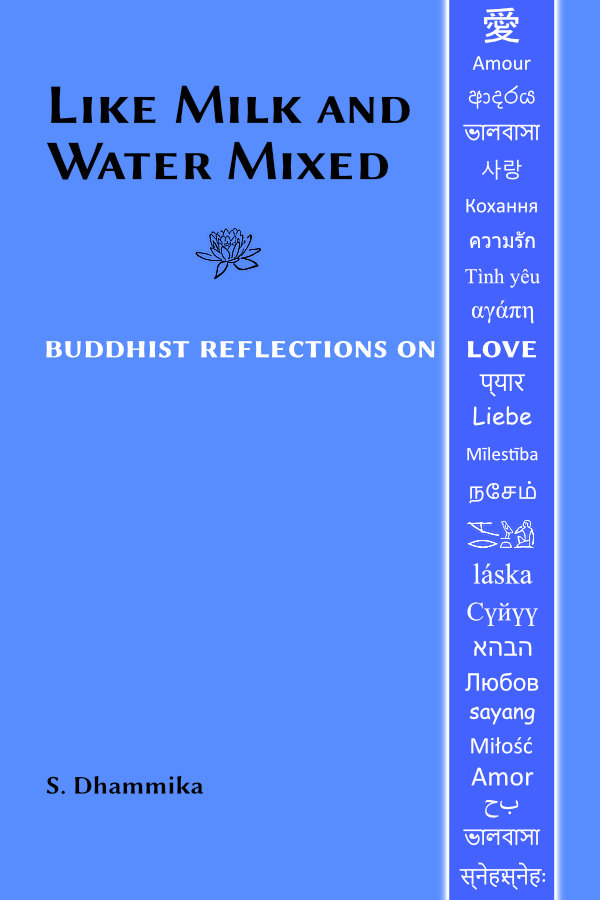
\includegraphics[scale= 2, trim= 0 0 0 0]{../_resources/book-data/milk/FrontLarge.jpg}

\newpage~\newpage~

\begin{center}
\vspace{2em}

\Huge\Titlefont\scshape{Like Milk and Water Mixed}\\
\vspace{0.5em}
\large\Titlefont\scshape{Buddhist Reflections on Love}\\

\begin{Large}
\vspace{4em}
\Titlefont\scshape{Bhante S. Dhammika}
\end{Large}


\vspace*{\fill}

\includegraphics[scale=0.06, trim = 0 13 5 0 ]{../_resources/images/icons/logo-enso-large}\\
\vspace{4pt}
\begin{small}
\scshape{Wisdom \& Wonders\\
Books}
\end{small}
\end{center}

\newpage
\begin{small}
\begin{sffamily}
\noindent Copyright © — Bhante S. Dhammika\\

\noindent © Shravasti Dhammika\\\noindent First Published in 2013.\\\noindent Second Edition in 2016.\\\noindent This Wisdom &amp; Wonders online edition 2024.\\\noindent Also Published by Pariyatti Publishing in Paperback 2024 (without SuttaCentral references).\\

\noindent\textbf{Attribution-NonCommercial-NoDerivatives 4.0 International (CC BY-NC-ND 4.0)}\\



\noindent\textbf{You are free to:}

\noindent Share — copy and redistribute the material in any medium or format


\noindent\textbf{Under the following terms:}

\noindent Attribution — You must give appropriate credit, provide a link to the license, and indicate if changes were made. You may do so in any reasonable manner, but not in any way that suggests the licensor endorses you or your use.

\noindent NonCommercial — You may not use the material for commercial purposes.

\noindent NoDerivatives — If you remix, transform, or build upon the material, you may not distribute the modified material.

\noindent No additional restrictions — You may not apply legal terms or technological measures that legally restrict others from doing anything the license permits.


\noindent\textbf{Notices:}


\noindent\textbf{You do not have to comply with the license for elements of the material in the public domain or where your use is permitted by an applicable exception or limitation.}


\noindent\textbf{No warranties are given. The license may not give you all of the permissions necessary for your intended use. For example, other rights such as publicity, privacy, or moral rights may limit how you use the material.}

\end{sffamily}
\end{small}


\tableofcontents

\mainmatter
\pagestyle{fancy}

			
			
			
\chapter[Acknowledgements]{\\Acknowledgements\markboth{Acknowledgements}{OOOO}}
Many people have helped me with this book. First and foremost of these is Anandajoti Bhikkhu, a genuine \textit{kalyāna mitta}. Through our almost daily emails he helped me with scriptural passages, and encouraged me to reconsider ideas I already had and suggested to me ideas I did not. Bhikkhu Brahmali helped correct and improve some of my Pāḷi translations. Nam Khim and my brother Charles gave their time and skills to improve my English style and grammar and get the manuscript ready for publication. The members and friends of the Buddha Dhamma Mandala Society—Dewi Taslin, Suhendra Sulistyo and Benny Luhur—helped me get the reading material I needed. Francine Lee and Michelle Tan read through several drafts of the book making many useful suggestions, and Padma was helpful in too many ways to mention. I am grateful to them all.


\chapter[Introduction]{\\Introduction\markboth{Introduction}{OOOO}}
The inspiration behind this book is the relationship I had with two people I became close to during the years I lived in Sri Lanka, Venerable Hinatinna Dhammaloka and Godwin Samararatne. Apart from the fact that the first of these individuals was a monastic and the second a lay person, both were remarkably similar in many ways. On first meeting them, it would have been easy to dismiss them as bland, uninteresting and slightly out-of-touch individuals. But on getting to know them better, observing how they behaved and listening to what they had to say, it soon became apparent that there was something very special about them. They were both smiling and kindly, softly-spoken, gentle and unassuming, and not just sometimes but seemingly all the time. In the years I knew them, I never heard either of them ever say anything unkind or disparaging to or about anyone. I never saw them being abrupt, haughty or impatient with anyone. And I never saw them flustered by anything that happened to them or around them. They acted and spoke lovingly towards everyone, and even when alone or when doing nothing they seemed to radiate an aura of love. It was only after I got to know Dhammaloka and Godwin that words like selflessness, detachment, kindness and love seemed to describe things that really existed rather than being just praiseworthy but remote concepts.


As a young man, Dhammaloka had been a social activist working amongst Sri Lanka’s rural poor. But by the time I knew him, he was already old and frail. He would sit all day with his eyes closed and a benign smile on his face. When someone came to see him he would greet them and engage in brief small talk before inquiring about the purpose of their visit, but without ever bothering to open his eyes to see who it was. Thinking that this was a little discourteous, I once asked him why he did it. He replied gently: “Does it matter who they are? Shouldn’t we treat everyone the same? The eye only sees the surface. It’s the heart that sees the inside. That’s what counts.”


In the months before his death, Dhammaloka became incapacitated and had to be looked after by the young monks in his monastery, some of whom found this rather irksome. On one occasion when another monk and I were taking him to the bathroom, the other monk caught my eye, pulled a face and made a mocking gesture towards the old man behind his back. By the time Dhammaloka emerged from the bathroom I had to help him back to his bed by myself, the other monk having gone to do something else. As I was doing so he leaned close to me and whispered: “They think I don’t know. I do know but I don’t mind.” Then he gave a chuckle.


Godwin Samararatne spent most of his life as a librarian.\footnote {For a short biography of Godwin Samararatne, see \cite{Samararatne 2007}} Since his youth he had been interested in Buddhism and by the early 1970s had started to become known to his friends and acquaintances as an unusually serene and meditative person. Being \textit{santa danta}, calm and controlled, is highly regarded in Sri Lankan society and Godwin was noticeably both. By the late 70s he had begun leading meditation classes, firstly for a small group of friends, then for larger numbers of people, and eventually in a meditation centre outside Kandy, the hill capital of Sri Lanka. By the time he died in 2000, he had become one of Sri Lanka’s best-known and esteemed meditation teachers.


Godwin was not particularly articulate. He was physically unremarkable and he had no academic or religious qualifications. And yet almost everyone who came into contact with him was affected by his kindness and compassion. He positively radiated a natural, joyful goodwill. The desire to help others free themselves from their emotional distress seemed to be his only ambition, and he possessed an extraordinary ability to do so. The advice he gave, the encouragement he imparted and the comfort he offered went straight to the heart because they came straight from the heart.


Neither Dhammaloka nor Godwin were teachers in any formal sense. Apart from anything else, they lacked the flair and eloquence usually associated with being a popular teacher. Neither did they claim any special authority or spiritual realisation. It was what they were that drew people to them. In Dhammaloka’s case, his position as a senior monk required him to give regular sermons, which he did up until a few weeks before his demise. No matter what he was asked to speak about—and in Sri Lanka it is common for the lay people organising sermons to request a particular topic—he would soon turn his talk to the subject of love, compassion and kindness. When someone would ask him to teach them insight meditation he would demur, saying that he did not have enough experience to explain it or act as a guide to it, although I suspect this was not actually the case. His main interest was encouraging people to practise Loving-kindness Meditation and to be more gentle, kind and considerate.


Being conversant in contemporary psychology and with a good knowledge of Western philosophy, Godwin’s approach to meditation was broader than Dhammaloka’s. It was based on the twin elements of mindfulness and love, or what he often characterised as mental clarity and emotional connection. He did not adhere to any particular meditation technique but encouraged each person to cultivate these two qualities using whatever techniques they were already familiar with or whatever suited their personality. But the instruction and advice he gave was not just effective because it was clear, simple and non-dogmatic. People took it to heart because he himself was so obviously mindful and filled with love. His personality gave an authenticity and immediacy to what he taught.


The personalities of Dhammaloka and Godwin inspired this book and some of their insights and ideas are incorporated into it. Some of what I have written has also been influenced by a familiarity with the Buddhist philosophy and meditation, by reading contemporary studies of love, and by my own thoughts and experiences.


Love is not necessarily an easy subject to write about. Studies of the subject by philosophers, psychologists and sociologists usually focus on one or another of its forms, most commonly romantic or conjugal love, and often use the word “love” without making it clear what is meant by it. Popular writing and discourse on the subject characteristically get lost in flood of clichés and ecstatic claims that evoke uplifting feelings but do not necessarily encourage realistic thinking. I have tried to define love in a way that will be recognisable to most people and which encompasses most of the experiences usually thought of as love. I had originally intended to write mainly about universal or brotherly love, what the Buddha called \textit{mettā}. But it soon became clear that this highest of loves is intimately connected with and perhaps necessarily preceded by other types. It is like pulling a thread out of a tapestry. As it comes it draws out so many other threads with it. Thus I was eventually led to explore nine different loves. I could have included other types as well but decided to limit myself to those loves about which the Buddha had something to say or which are relevant to practising Buddhism.


As my reading and reflections proceeded, I soon became aware that a swirl of myths surround love. The most noticeable of these myths is that love is a widely felt and easily evoked experience. It is celebrated endlessly in song and story; it is ardently professed, hailed as the solution to many—sometimes all—human problems. Yet while love is not necessarily rare, it is certainly not as common or as enduring as is generally supposed. The divorce statistics from most developed countries show that between 40 and 55 per cent of marriages end in divorce, many of them acrimonious. And people who stay married do not always still love their spouses. The endless sorry parade of cases that come before family and small claims courts shows that relationships between siblings, in-laws, neighbours and friends are not as enduring as we so blithely suppose. If spousal love, familial love and love of one’s neighbour so often turn sour, then what of universal love? It is a tragic paradox that some of the great individuals who have spoken or written so eloquently and movingly about love have sometimes shown a miserable lack of it in their relationships and their affairs. Martin Luther was able to deliver one of the finest sermons even given on 1 Corinthians 13 while at the same time hating the Jews with a fury almost equal to Adolf Hitler’s.


Mahatma Gandhi, the epitome of gentle, kindly patience in many people’s minds, was demanding of his wife and sons to the point of cruelty. Our religious institutions place an accepting, forgiving love as the centre of their teaching, and yet they cannot put aside their theological differences and worship the same god in unity.


None of this invalidates the importance of love or diminishes its beauty. But it should cause any thoughtful person to pause and consider that having love and sharing it with others is no easy matter. It takes commitment and effort, self-honesty and perhaps even sometimes considerable self-sacrifice. It is far easier to glorify love than to allow it to fill our hearts and guide our thoughts, speech and actions. I have kept this sometimes overlooked truth in mind during my reflections and have tried to speak about love realistically.


The good news is that almost everyone has loved or has tried to love at some time or another. This can be taken as compelling evidence that all of us are capable of love, and perhaps even that it is an innate potential we all possess. Certainly Buddhism would agree with this and add to it, saying that our love can go beyond being projected to a few people to being pervaded to everyone, indeed to all sentient life. The Buddha taught a series of spiritual exercises meant to do exactly this—to strengthen the love we already have, transmute it into a higher love and then make it all-embracing. Three chapters in this book have been devoted to explaining these spiritual exercises. These reflections are based on the transcripts of a series of talks I gave in Singapore in 2012. While preparing these talks I read a selection of contemporary writings on and studies of love. The ones I found most helpful and which I would recommend to anyone wanting to explore the subject more deeply are Irving Singer’s magisterial three-volume \textit{The Nature of Love} (\cite{Singer 2009a}, \cite{Singer 2009b}, \cite{Singer 2009c}) and his \textit{Philosophy of Love} (\cite{Singer 2009d}), Pitirim Sorokin’s \textit{The Ways and Power of Love} (\cite{Sorokin 1954}), Erich Fromm’s perennial classic \textit{The Art of Loving} (\cite{Fromm 1956}), and Simon May’s \textit{Love: A History} (\cite{May 2012}). Robert Sternberg’s and Michael Barnes’ \textit{The Psychology of Love} (\cite{Sternberg and Barnes 1988}) helped me navigate my way through modern research on the subject, and others might find their book helpful too. Adam Phillips and Barbara Taylor’s wonderful little study \textit{On Kindness} (\cite{Phillips and Taylor 2009}) is also an insightful read. Of Buddhist authors, I would particularly recommend Nyanaponika’s small but excellent \textit{The Four Divine Abidings} (\cite{Nyanaponika 1958}), several of Thich Nhat Hanh’s books, most notably \textit{Cultivating the Mind of Love} (\cite{Hanh 1996}) and \textit{Teachings on Love} (\cite{Hanh 1998}), and Sharon Salzberg’s \textit{Loving-kindness: The Revolutionary Art of Happiness} (\cite{Salzberg 1995}). The Dalai Lama’s \textit{An Open Heart} (\cite{Dalai Lama 2001a}) and \textit{The Compassionate Life} (\cite{Dalai Lama 2001b}) are also essential reading.


\chapter[1. What is Love?]{chapter 1\\What is Love?\markboth{What is Love?}{OOOO}}
Few human experiences have been more pondered over, more discussed and more longed for than love. Most of the songs on the radio are about it; a good percentage of popular literature and film deals with the subject. Mystics, theologians, philosophers and more recently psychologists have tried to explain it. In the build-up to some conflict, or after, religious leaders and other concerned individuals say such things as “If only we can learn to love each other….”


The Bible claims that the essence of the most important being in the universe, God, is love. Clearly this experience, whatever its nature, is a major concern of humanity and always has been. But despite all the attention that has been given to it, exactly what love is remains elusive. We can say that we love our parents, our children, and our neighbour. Although it is clear that the loves we have for these different individuals share common features, it is just as clear that they must have important differences too. Loving a spouse includes sexual intimacy while loving a sibling or a child does not. It is quite normal to say things like “We loved Spain” or “I love Mozart” but again the components of such loves must be very different from those felt towards a flesh-and-blood person. Complicating matters further is the fact that people sometimes say they love and even think they love when they actually do not. I have heard conversations starting with “I really love you but …” followed by a list of bitter recriminations and angry complaints.


So what is this thing we call love? Many descriptions of love are more panegyric or accolade than clarifying. “Love is the poetry of the senses.” “Love is the beauty of the soul.” “Love is the joy of the good, the wonder of the wise, the amazement of the gods.” Sayings like these, and any dictionary of quotations will include many of them, suggest that love calls forth strong sentiments and colourful fancies, but they do not really tell us anything useful about it. Moving from warm ambiguity to cool-headed precision, there are plenty of attempts to define or describe love. Probably the most famous of these from the Western spiritual tradition is the one given by Paul of Tarsus in his epistle to the Corinthians. Paul used the Greek word agape, which is usually rendered as charity or love or sometimes brotherly love.


\begin{quote}


“Love is patient, love is kind. It does not envy, it does not boast, it is not proud. It is not rude, it is not self-seeking, it is not easily angered, it keeps no record of wrongs. Love does not delight in evil but rejoices with the truth. It believes all things, hopes all things, endures all things.”\footnote {1 Corinthians 1, 13}




\end{quote}
Of the 14 characteristics given here by Paul, more than half are negatives, that is, they tell us what love is not or what it does not do, rather than what it is and does. This is probably no accident. Paul realised, as many have before and since, that it can be easier to define some things by what they are not rather than what they are, and this is particularly true for a multifaceted quality like love. The Buddha occasionally did the same, using words for love such as \textit{avyāpada}, literally hatelessness, or \textit{adosa}, non-ill-will. As for love’s positive qualities mentioned by Paul, most people would agree with him that patience, kindness, humility, and unselfishness are features of love, although I suspect that others would associate believing and hoping everything more with naivety and wishful thinking.


An early Buddhist text, the Culla Niddesa, defines love like this: “Love means having a friendly nature and behaving with friendliness.”\footnote {\textit{Mitte vā bhavā mittassa vā esā pavattī ti pi mettā}, Culla Niddesa 117.} This would seem to discount the depth of feeling that is usually associated with romantic and companionate love and more closely resembles what we might call affection or goodwill. The 5<span class='superscript'>th</span> century Indian Buddhist scholar Buddhaghosa was being more specific when he wrote: “Love is characterised as promoting the welfare of others and its function is to focus on their welfare. It manifests as the removal of annoyance and its proximate cause is seeing the lovable nature of beings. It succeeds when it makes ill-will subside and it fails when it gives rise to clinging attachment.”\footnote {Vism. 318.} Although rather stilted, Buddhaghosa’s understanding here is significant in that it sees love as being primarily about doing something to and for others, as being motivated by concern for their welfare (\textit{hitākārappavattilakkhaṇā mettā}). Interesting too is his idea that by their very nature living beings are lovable or fit objects of love (\textit{manāpabhāva}).


When we get to modern times we begin to have more penetrating explorations of love. The Oxford Dictionary says love is “an intense feeling of deep affection” or “a deep romantic or sexual attachment to someone.” But surely there is more to love than just attachment and sexual longing. Sigmund Freud observed love with a sceptical and jaundiced eye and dismissed it as “aim-inhibited sex.” For him love was a more refined form of the sexual drive. Martin Luther King called love a “recognition of the fact that all life is interrelated. All humanity is involved in a single process, and all men are brothers.” It is unlikely that anything like this passes through the minds of two people head over heels for each other. The popular writer M. Scott Peck understood love to be “the will to extend one’s self for the purpose of nurturing one’s own or another’s spiritual growth.”\footnote {\cite{Peck 1997}, p.69.}


The problem with this and indeed King’s definition is that they pretty much exclude romantic love and close friendship. Many people are involved in genuinely loving relationships while having no spiritual aspirations. The psychiatrist and writer Colin Murry Parkes defined love as “the psychological tie that binds one person to another over a lasting period of time.”\footnote {\cite{Parkes 2009}, p.2.} This is broad enough to embrace most of the diverse expressions of love, but it could also define hate. Members of the Ku Klux Klan probably share a common psychological tie but it is nothing like what most people would think of as love.


Some modern thinkers see the defining feature of love as “robust concern,” “attachment” or the “bestowal of value.” Again most types of love have these features but they have other important or more pronounced ones as well. Other observers have emphasised that love is primarily an attitude of kindness, including towards unpleasant people. The English eccentric Quentin Crisp used to say that “love is making an effort to be nice to the people you do not like.” This and similar definitions imply that love is not necessarily a warm feeling connecting with another or others but an ongoing effort to break, suppress or resist the tendency to strike back at people we find objectionable.


All these definitions and descriptions are good as far as they go, but not all love is romantic or divine, an impulse or an act of will, an emotion or an art. Perhaps another reason why love is so difficult to pin down and why there is such a wide variety of opinions about it is because the word “love” is used so casually. The feelings and attitudes implied by the statement “I love Chinese food” would have little in common with those implicit in “We love our daughter.” The word “love” is frequently used when “like,” “favour” or “prefer” would actually be more appropriate. Then there is the problem of boundaries, of where states such as affection, closeness and fondness end and love begins.


Would it be possible to craft a definition of love that could embrace all its colours and contours, its manifestations and modalities? The reflections that follow are based on the understanding that \textbf{love is an active interest in, care for, empathy towards and desire for intimacy with another or others, usually accompanied by positive feeling}. This definition attempts to include all the more commonly recognised and agreed upon cognates of love and most of the mental states usually so labelled. It draws on an understanding of Buddhist philosophy and psychology but is also informed by my experience as a counsellor and some familiarity with contemporary studies of love. Let us consider a little more deeply these five defining characteristics which together constitute love.


To be interested in something means having one’s attention engaged by it and wanting to know it better. When two people first fall in love they spend much of their time getting to know each other, exploring each other emotionally and physically. At first their interest is as much curiosity as anything. Later, knowing their beloved better, their habits, likes and dislikes and then taking them into account, this interest allows them to please their beloved and thus strengthen the growing bonds between them. Couples who have been happily married for years say, probably truthfully, that they often know what their partners are going to say before they say it. During their years together they have got to know each other in ways that even close acquaintances never could.


\begin{epigram-2}
There is only one true love but there are many good imitations.
\end{epigram-2}

\begin{epigram-2-cite}
—La Rochefoucauld
\end{epigram-2-cite}

A doctor who is deeply concerned for his or her patients will try to know everything about them and the illness that afflicts them. While young lovers will be constantly revealing information about themselves and soliciting it from their beloved, the genuinely caring counsellor might say very little to the people who have come to them for help. He or she will speak little but listen intently, once again being interested in their clients in the hope of understanding them. Someone who has come to love God will pray earnestly and study the scriptures carefully in the hope of knowing God’s will and what he wants of them. It is commonly said that love is blind and that is certainly true of the type that suddenly blazes and then quickly burns itself out, often leaving cinders of anger and heartbreak. But the love that endures does so because it is interested in the loved object, and this interest delivers knowledge and from that comes understanding.


Care is both an attitude and a behaviour. People who care are not just willing to take upon themselves some responsibility towards those they care about but they are happy to do so. Care is the opposite of being “careless” or “uncaring,” the first implying indifference and the second callousness, each of them the antithesis of love. As an attitude, genuinely caring for others might take the form of seeing to their needs, helping them in various ways, mentoring them or giving them advice. It may even involve putting restrictions on them, although this would not be done out of a desire to dominate or control but to protect the loved one until they can become responsible for themselves.


The Buddha manifested all the signs of being a caring teacher. He was deeply concerned that those who came under his tutelage should grow spiritually. Once he advised his senior monks not to reprimand young novices for their each and every mistake. To do so, he said, might dishearten them, cause them to lose “even the little faith and the little love” they had and then leave. He put it this way: “If a man had only one eye his friends and family, kith and kin, would take great care of his good one, thinking ‘Let him not lose that eye too.’”\footnote {\href{https://suttacentral.net/mn65/en/sujato\#28.1}{MN 65:28.1–28.9} [PTS: M.I,444].} He was asking the seniors to care for their juniors out of concern for their spiritual welfare. When the monk Channa confessed to Sāriputta that his prolonged and painful illness was making him seriously consider suicide, Sāriputta said to him: “Do not kill yourself Channa. Live. I want you to live. If you do not have suitable food or medicine, I will get them for you. If you do not have suitable care, I will take care of you. But do not kill yourself. Live. I want you to live.”\footnote {\href{https://suttacentral.net/mn144/en/sujato\#6.1}{MN 144:6.1–6.7} [PTS: M.III,264].}


Again these were the words of someone who deeply cared about another and wanted them to flourish. Generosity and service are sometimes motivated by a sense of duty or by religious obligation but they flow naturally from the loving heart. We delight in sharing what we have with our loved ones and we are quick to respond when they are in need. We never see this as a duty, an obligation or a burden. Caring behaviour is love transmuted into giving, sharing and helping.


Love’s third defining characteristic, empathy, is that special human ability to get out of oneself and enter into the thoughts and feelings of others. In Buddhism this quality is called \textit{dayā} or \textit{anuddayā}. While interest in someone gives us a “head” knowledge of them, empathy gives us a “heart” knowledge: we come to know them and thus connect with them, from the inside as it were. The Buddha was referring to being empathetic when he counselled “put yourself in the place of another”\footnote {\textit{attānaṁ upamaṁ katvā}, \href{https://suttacentral.net/dhp129/en/sujato}{Dhp 129}.} and when he asked us to think: “as am I so are others, as are theirs so am I.”\footnote {\textit{yathā ahaṁ tathā ete, yathā ete tathā ahaṁ}, \href{https://suttacentral.net/snp3.11/en/sujato\#27.1}{Snp 3.11:27.1–27.4} [PTS: Sn.705].} To be empathetic requires a sensitivity towards others and, perhaps paradoxically, even a certain degree of detachment from ourselves. To the degree we are involved in our own feelings, concerns and perspectives, we are less likely to notice those of others and thus less likely to be able to empathise with them.


Intimacy is a physical and/or psychological closeness to someone or something. The first thing that springs to mind in relation to love and intimacy is sex, and indeed sexual intimacy is an important component of some types of love. But physical intimacy can manifest itself in other types of love too, and in other ways. When we see a child, even if it is not our own, we might have a strong desire to cuddle it or give it a hug. A warm handshake and a smile let a stranger know he or she is accepted and welcomed. When we see someone grieving or frightened, we can be moved to take their hand or put a comforting arm over their shoulder. If we know someone well, we might hold them in a friendly embrace or kiss them. Physical intimacy with animals is not unknown either. A friend of mine is inordinately fond of his dog and allows it to lick his face. I have also often seen him snoozing on the couch with his dog curled up on his chest. Physical proximity and touch can both express and reinforce love. A head on the shoulder, arm around the waist and walking hand-in-hand are all common expressions of loving intimacy.


It is possible to be emotionally intimate too. The Buddha said that one of the characteristics of a loving friendship was mutual self-disclosure, the sharing of secrets.\footnote {\href{https://suttacentral.net/dn31/en/sujato\#23.1}{DN 31:23.1–23.3} [PTS: D.III,187].} We feel privileged and trusted when our loved ones tell us things they have never told anyone else. Likewise, we like to confide in those we love. It is another way of saying that they are special enough for us to invite them into our innermost being. Another form of emotional intimacy is freely expressing our deepest feelings with those we love. We feel we can cry in front of them, sometimes cry with them or tell them our fears and desires. Sharing objects that are ordinarily reserved for personal use is also a type of intimacy.


It has been mentioned above that empathy and a desire for intimacy with another or others are amongst the defining characteristics of love. This being so, it is not really possible to love inanimate objects. No matter how strong the desire for intimacy is, it cannot happen with something that has no inner life. We can be intensely interested in our country, studying its history, geography, flora and fauna so well that we know it thoroughly, but we cannot know any dimension of it beyond the physical because it does not have one. Again, no matter how much we may “love” hamburgers, Cuban cigars or Cashmere sweaters, we cannot empathise with them, we cannot be intimate with them and they have no means of doing that with us. Although reciprocity is not required for love to be present, responding positively to someone’s love usually draws more love out of us, intensifying our love for them and theirs for us. Non-living things cannot return any interest or affection we might have for them.


What about plants? We may say that we love the majestic old tree in the local park or the roses climbing along our garden fence, but can we really “love” them the way we love grandma or the family cat? The Buddha described plants as life forms with one faculty (\textit{ekindriya}) although he did not specify which faculty they possessed. Daisies follow the sun as it moves across the sky and mimosas close their leaves when touched, but to the best of our knowledge plants do not have feelings or emotions in the sense that humans and other animals do. According to the definition given above, being loving, giving love and receiving it are privileges of living beings. To love is to live.


Whether we love God or our spouse, the neighbours or the family dog, whether we are receiving it or bestowing it, love often makes us feel very good. In ways that are not always easy to explain, love seems to enrich our lives, making it worthwhile despite all its complications. Psychologists tell us that those who have been deprived of love in early childhood often lack the ability to relate successfully with others when they mature. Both giving and receiving love seem to be essential factors in growing into a well-balanced, happy human being. For many people, falling in love will give them the most ecstatic feelings they ever experience. Successful marriages and close friendships make the individuals involved happier; they live longer. In survey after survey, people report that their greatest joy in life is their children. For many people their fondest and most treasured memories are not about acquiring worldly success or material gains but the special moments they have shared with loved ones and friends.


Other ways of being loving impart happiness too. If we are friendly, kind and helpful towards others they will usually respond in the same way and this elevates the general level of good feeling in all concerned. Doing a favour for someone and having them thank us makes us feel pleasantly energised. Sharing things with someone and having them express their appreciation to us can likewise lift our mood considerably. This does not mean that if we are good, kindly and loving that we will never feel down. Romantic relationships can be emotionally tumultuous, even good marriages have their “ups and downs,” and a kind act can be rudely rebuffed leaving us hurt and indignant. But it is a safe generalisation to say that those with much love experience much happiness.


Once I found a purse on the footpath. I picked it up, looked inside and discovered that it contained documents, a few keys and a large amount of money. I was not the slightest bit tempted to keep the money, but having to go to all the way to the police station to hand the purse in would have been a considerable inconvenience. I continued on my way, going through the documents to see if I could find a name or a telephone number, which I did. I noticed a telephone box ahead of me and decided to ring the number I had found. I got the woman named in one of the documents and her relief on hearing that her purse had been found was very obvious. I said I would wait while she drove to the telephone box to meet me. When she arrived she was nearly overwhelmed with gratitude. She told me all the problems she would have had to face if she had lost her documents and keys, and that the money was essential for some pressing need. We talked for a while and before parting she took my hands and said with deep feeling: “Thank you! Thank you! Thank you so much!” I felt very happy and even as I write this nearly 20 years later, I still feel a mild glow as I remember it.


Why does doing good to others, being kind and considerate towards them, usually make us happy? In the incident related above I recognise that the woman’s effusive gratitude probably enhanced my self-image, and having one’s ego inflated is always gratifying. However, this cannot be the whole story. Sometimes we help others anonymously or receive no thanks for the good we have done, and yet we still feel good.


It seems that a combination of two things impart happiness when we are kind to others—simply knowing that we have eased a fellow creature’s path through life, even if just a little, and the ability to be happy in the happiness of others, a mind state the Buddha called sympathetic joy (\textit{muditā}). The Buddha recognised this phenomenon although he did not explain it. “One rejoices here, rejoices after death, rejoices both here and hereafter. One rejoices recalling the good deeds one has done.”\footnote {\href{https://suttacentral.net/dhp16/en/sujato}{Dhp 16}}


Religious teachers, philosophers and moralists are always encouraging us to be kind to others, assuring us that it will make us happy, but I suspect no-one is listening to them. When one person reaches out to help another I doubt that somewhere in the back of their mind they are thinking “Oh goody! A chance to make myself happy.” It seems that most of us know without being told that kindness and goodwill to our fellow beings leads to happiness.


\begin{epigram-2}
What most people call love is just a pleasant feeling.
\end{epigram-2}

\begin{epigram-2-cite}
—Ajahn Chah
\end{epigram-2-cite}

However, being loving does not inevitably go in tandem with positive feelings. It is possible to do good to others with kindly intentions while remaining emotionally neutral. A nurse can care for her patients with great tenderness and dedication while remaining business-like and emotionally detached. Occasionally she may experience happiness and a sense of satisfaction when she considers that she is a good nurse or when someone expresses their appreciation to her. But such feelings need not be there every time she cares for her patients. A spouse or a parent can have the deepest love for their partner or children while sometimes being exasperated, annoyed or bored by them, even as they are helping them, making sacrifices for them or encouraging them. Forgiveness is widely considered to be an act growing out of love. However, when we resolve to forgive someone or when someone asks for our forgiveness and we grant it, we may still feel resentment or anger towards them. In fact, forgiveness is usually thought of as only having occurred when it is given despite hurt feelings. We notice our love more when it is coupled with positive feelings but the two need not go together. Love is not a feeling although it often forms an ensemble with a strong positive feeling. Love is an attitude, a behaviour and a way of relating to others. It is only when feelings are mistaken for love or are seen as its core that our relationships become complicated by jealousy, attachment and dependency. We humans have a strong proclivity to cling to feelings.


It has been said above that love is the interplay of interest and care, empathy and desire for intimacy which together create a connection between living beings and is often associated with positive feelings. It has also been said that all these components have to be actively expressed to qualify as love. In other words, love is not an idea any more than it is something we feel and then sit back and enjoy. It implies some form of physical engagement, being set in motion, being “moved.” The Buddhist scriptures comment that a mother’s heart trembling like leaves fluttering in the breeze when she sees her child after a long absence.\footnote {\href{https://suttacentral.net/ja532/en/francis?reference=main/pts#pts-vp-pli328}{Ja 532} [PTS: Ja.V,328].} But this is not the movement meant here. It means that when we truly love someone we physically and psychologically interact with them to the point where we influence their life. This underscores what the Buddha was referring to when he spoke of “loving acts of body.”\footnote {\textit{mettena kāyakammena}, \href{https://suttacentral.net/dn16/en/sujato\#5.14.5}{DN 16:5.14.5} [PTS: D.II,144].} The Bible also emphasises that love has to flow from the heart so as to move the hands. “If anyone has material possessions and sees his brother in need but has no pity for him, how can the love of God be in him? Dear children, let us not love with words or tongue but with actions and in truth.”\footnote {1 John 3,17-18.} Love is as much a behaviour as it is an attitude.


People often talk about what they call “unconditional love.” If we can prevent the warm glow we feel when we hear this term from stopping us thinking carefully and clearly, we may have to reconsider the reality of so-called unconditional love. People have told me that their partner loves them “unconditionally” but two or three years later I hear that their relationship is having problems or even that they have separated. Some conditions, some changes in circumstances, must have altered the love they felt for each other. I recently read an article in a magazine subtitled “A mother’s unconditional love for her child.” It told of a woman’s struggles to look after her severely ill daughter and the many sacrifices she made while doing so. It was a poignant and moving story. But while this mother remained devoted to her child despite the enormous challenges, her love does seem to have had its conditions. There is little doubt that she did everything she did because the child was hers, that is, that her love and devotion were aroused by her maternal instincts. It is unlikely that she would have made similar sacrifices for a complete stranger’s child. In one place in the article the woman said “I could never have done it without the support of my husband,” again indicating that what she did was made possible in part by the help she received from another person.


This is not to deny the woman’s tremendous courage, devotion and self-sacrifice but only to point out that her love, like all states, was conditioned and influenced by various factors. It would seem that even divine love, the love of God, any god, has its conditions. We are told that God will forgive our sins but only on condition that we believe in him, repent and genuinely try to reform ourselves. If we die without having fulfilled these conditions God’s subsequent judgement will result in him abandoning us to a very unpleasant fate for a very long time. Even if this is the result of choices we have made, it still makes God’s love different from what it would have been otherwise.\footnote {See Simon May’s interesting comments on this subject—\cite{May 2012} pp.106-118.}


The Buddha said that everything in the universe existed due to the coming together of a complex web of causes and conditions, and love was no exception to this. The type of love we are capable of, its strength and sustainability, is conditioned by multiple psychological factors such as our emotional make-up, our will, our beliefs, and so on. It may also be conditioned by external factors such as our social norms, the people we come into contact with and the nature of the relationships we have with them. However, to accept that our ability to love and the love we express is conditioned does not belittle it but only lets us look at it with clearer eyes. If we elevate love or indeed anything out of reality, this will prevent us from understanding it fully.


I am able to read the scriptures right now at 10 o’clock in the evening because I have light. I have light because the light bulb is working and I paid last month’s power bill. Is my ability to read the scriptures diminished in some way simply because it depends on certain conditions? Does it suddenly become impossible to learn from or be inspired by the Buddha’s words because reading them is made possible by the light bulb? If tomorrow I am charitable towards someone as a result of what I read, does that act become inconsequential just because I paid the power bill? I do not think so. Love is not robbed of its goodness and its majesty because it is conditioned.


While love is conditioned, it is also true that some love is more conditioned than others or that it is conditioned by different factors. The less conditions love requires to awaken, to grow and to express itself, the less conditions thwart it and hold it back, the more exalted it is. Romantic love requires sex or the promise of sex to stay alive and usually fades if one of these is not forthcoming. Conjugal love can be strained by long separation and rarely survives betrayal even if it does not end in divorce. Likewise, loving friendship needs to be continually nourished by trust, loyalty, shared interests and so on. Except perhaps for the highest spiritual love, most other types need to be reciprocated. What we really mean by unconditional love is a love that gives itself easily, that persists despite obstacles, that has few expectations, and that makes few demands.


\chapter[2. Two Hearts Beating as One]{chapter 2\\Two Hearts Beating as One\markboth{Two Hearts Beating as One}{OOOO}}
Even people who usually do not think too deeply about it or are little aware of what goes on within their hearts recognise that there are different types of love. It is quite normal to speak of true love, puppy love, hard love, love at first sight, the love that dares not speak its name, platonic love, unrequited love, love-hate relationships, and love with open eyes. Psychologists refer to “love styles” or “bond varieties.” We also have many words and phrases for those mind states that are not love but which hover around its edges—affection, fondness, warm feelings, kind regard, closeness, liking, devotion and so on. The Buddhist scriptures contain numerous words for love such as \textit{ādara}, \textit{atthakāma}, \textit{dalhabhatti}, \textit{hita}, \textit{kāma}, \textit{lokassādara}, \textit{manāpa}, \textit{matteyya}, \textit{mettā}, \textit{paṭibaddhacitta}, \textit{paṭisanthāra}, \textit{pema}, \textit{petteyya}, \textit{piya}, \textit{sambhajeyya}, \textit{sampiyāyanā}, \textit{siniddha} and \textit{sineha}. Some of these words are synonyms, while some refer to distinct types of love. Although it is not always easy to find exact English equivalents for some of them, others can be identified with certainty. For example, \textit{paṭibaddhacitta} means infatuation, \textit{petteyya} is paternal love, \textit{kāma} is erotic or sensual love, and \textit{sampiyāyanā} might mean something like endearment or affection. Let us explore some of the more distinct types of love mentioned in the Buddhist tradition.


Most people have heard the term “brotherly love” or “universal love” and are ready to praise it without necessarily ever having felt it or even having tried to evoke it within themselves. Deeply religious people say they feel God’s love but those who do not believe in the supernatural find it hard to understand what they are talking about. Some people have a tender spot in their hearts for animals while others are unmoved by them. But almost everyone has fallen in love at one time or another, perhaps several times. So for most people “love” is that exciting and sublimely agitating urge for intimacy with another, felt vaguely in the area of the solar plexus. Discussions on love almost always include something about what is called erotic love, romantic love or amour, \textit{eros} to the Greeks, \textit{kāma}, \textit{lokassādare} or \textit{rati} in Buddhism. This is the love that makes the world go around, as the saying goes. It is the love that has inspired some of civilisation’s greatest literature, art and music. It is the love everyone longs to experience and hopes will last forever.


Falling in love as we understand the experience today was not very common during the Buddha’s time, any more than it was in other ancient cultures. The prelude to and purpose of marriage was not love. People married to preserve property and produce legitimate progeny, and therefore most marriages were arranged by parents. Young people were paired off soon after they reached sexual maturity so they had very little opportunity to fall in love. If love grew, it did so after the wedding. Despite this, sometimes young people did manage to fall in love with each other or sometimes those already married fell in love with someone other than their spouses. Illicit romantic and sexual relationships happened despite the lack of opportunities and strong social disapproval.


Today romantic love commonly blossoms quite suddenly. One person sees another, is immediately attracted and then falls in love with them. He or she then attempts to make contact with the person they desire in the hope of attracting their attention and getting to know them better. If things go as hoped and their interest is reciprocated, a romance will result. If shyness, insurmountable social differences or other barriers make close contact with the loved person impossible, they may secretly worship them from afar, pining for them and dreaming or fantasising about a relationship with them.


Of course, not all love starts by suddenly “falling” into it; sometimes it grows slowly. The scriptures identify at least four stages in this gradual awakening. It begins with seeing, seeing leads to association, association leads to intimacy, and intimacy leads to amorousness.\footnote {\textit{dassana}, \textit{samsagga}, \textit{visāsa}, \textit{otāra}, \href{https://suttacentral.net/an5.55/en/sujato\#1.2}{AN 5.55:1.2–1.10} [PTS: A.III,67]. What is translated here as amorousness (\textit{otāra}) could also be rendered as “getting a chance.”} Romantic love can last for weeks or months, although if requited it will last much longer. But sooner or later, it either fades, sours into dislike, or becomes more settled and evolves into conjugal love.


\begin{epigram-2}
Sensuality makes love grow too quickly, so that the root remains weak and is easy to pull out.
\end{epigram-2}

\begin{epigram-2-cite}
—Friedrich Nietzsche
\end{epigram-2-cite}

Romantic love has all the defining characteristics of other types, although in a much more exaggerated and unruly form. Couples in love are intensely interested in each other; much of their time together is spent talking to each other about the minute details of their lives, likes and dislikes, hopes, interests and dreams. “What are you thinking?” a young woman will sometimes say to her beloved.


Lovers come to care about each other too, about each other’s happiness and well-being and particularly that the love they share continues and grows stronger. They empathise with each other, and in romance this is usually described as “two hearts beating as one.” Desire for intimacy is heightened. During the first flush of love, the couple involved can hardly bear to be out of each other’s sight and the desire for sexual intimacy often has a desperate, urgent quality to it. In fact, so closely is romantic love associated with sex that the physical act of sex is commonly called “making love.” In no other type of love is positive feeling so dominant, sometimes overwhelmingly so, although it is commonly punctuated by episodes of despair and distress, anxious longing and shattered hopes. Arguments followed by reconciliations, or separations ending in reunions, seem only to intensify the partners’ attachment to and longing for each other’s company. Sometimes couples will even create such situations so that they can savour the reconciliation. The scriptures say: “When a couple or a husband and wife frolic in private with romantic love they chide each other—‘Dear One, you don’t really love me; your heart is elsewhere’. They chide each other like this falsely so that they can then love each other more passionately.”\footnote {\href{https://suttacentral.net/ja542/en/cowell-rouse?reference=main/pts#pts-vp-pli378}{Ja 542} [PTS: Ja.VI,378]. A Latin epigram says something similar: “\textit{Amantium irae amoris integratio est},” “Lovers quarrels are the renewal of love.”}


The bliss of new love can be strong enough to affect a person’s appearance and behaviour. It can give them a smiling, dreamy, faraway look or a twinkle in their eyes. It can make them appear preoccupied and uninterested in normal activities or give them a spring in their steps, at least when their relationships are proceeding smoothly.


Apart from possessing the defining characteristics that all loves share, romantic love has its own unique features. It is initially triggered by visual contact. “Love goes to one who is seen, there is no attraction to one who is not seen.”\footnote {Rāmāyaṇa V,26;39.} Its primary focus is the body; for males the face, breasts and hips, and for females the face, shoulders and chest. Certain body shapes evoke more desire than others, depending on cultural norms, and some of these can be very peculiar. In China until the beginning of the 20<span class='superscript'>th</span> century, males found abnormally small female feet intensely erotic. Now most people would be revolted by such deformities. Only a hundred years ago in the West, a pale complexion was thought of as beautiful. Now being tanned is the fashion. In ancient India both men and woman were erotically aroused by what was called the \textit{tanuromaraji}, the line of hair going from the pubis to the navel.


Nowadays men and women are prepared to undergo painful procedures to remove such hair because it is deemed unsightly. In contemporary Western society a rounded profile in a male’s arms will be attractive to a female, although a similarly rounded form in the abdomen will be a turn-off. Full rounded female breasts are desirable to a male but similarly large and rounded buttocks might be perceived as unattractive. Just how particularly romantic love can be about physical features is suggested by this description of female beauty from the scriptures. To be alluring to a man, a woman had to be “fifteen or sixteen, not too tall and not too short, not too thin and not too fat, not too dark and not too fair.”\footnote {\href{https://suttacentral.net/mn13/en/sujato\#18.2}{MN 13:18.2} [PTS: M.I,88].} The presence or absence of even small and otherwise insignificant features or details can make the difference between arousal and disinterest. The pathways of eroticism and romance are not always easy to fathom.


Another important feature of romantic love is its tendency to distort perception. Buddhist scriptures refer to being blinded (\textit{kāmandha}), befuddled (\textit{kāmamatta}) or intoxicated (\textit{kāmāsava}) by love. A person in love sees everything about their beloved as exceptional. A young man might say of his beloved: “Her hair is like silk,” “Her teeth are like pearls,” or “Her eyes sparkle like stars.” But when we observe her various body parts they do not seem to be significantly different from anybody else’s. People in love do not say things like this in flights of ecstasy; they really believe what they say. Love makes their eyes see things in a different if unrealistic light, which can lead to problems. When the wild passion fades as it inevitably must, and the loved one is seen with a more critical eye, disappointment can set in. What before was a cute or delightful quirk may become an annoyance. When one person is besotted by another who does not love them with equal passion or perhaps not at all, they can be open to being exploited by them. They might be asked for and gladly give expensive gifts, money and favours. The besotted person’s family and friends can see what is happening, that the love-struck is being taken advantage of, but they themselves cannot see it. Romantic love can be, as they say, blind.


Most of all, romantic love seems to operate outside the will. The term “falling in love” is a very appropriate and descriptive one. As in actually tripping or being pushed and falling, you cannot stop until you hit the ground. A person does not choose or decide to fall in love; a surge of dopamine, oxytocin and other hormones in the system decides for them. The pull of romantic love and sexual delight, the promises they whisper in the ear, can be very hard to resist. Occasionally one of the Buddha’s monks would appear to be progressing well, developing calm and detachment, experiencing the joy of simplicity and silence. Then suddenly “he hears that in a particular village or town there are women or maidens fair to look upon, lovely, with the wondrous beauty of a lotus. When he hears this he loses heart, falters, cannot keep strong, and is unable to continue the training. Then he acknowledges his weakness, gives up the training and returns to the lay life.”\footnote {\href{https://suttacentral.net/an5.75/en/sujato\#6.1}{AN 5.75:6.1–6.10} [PTS: A.III,90].}


\begin{epigram-2}
In real love you want the other person’s good. In romantic love you want the other person.
\end{epigram-2}

\begin{epigram-2-cite}
—Margaret Anderson
\end{epigram-2-cite}

Abandoning the life of a celibate monk or nun for romance is one thing, but people sometimes take extraordinary risks or act with unbelievable irresponsibility because they are under the spell of sexual desire or romantic love. It is romantic love’s unruly, distorting and distracting qualities that made the Buddha very cautious of it, and of course he was by no means the only one. The Jains, Hindus, Stoics, Gnostics, and the early Christians all saw romantic entanglements as pulling one’s energy and attention away from more spiritual aspirations. Jesus said nothing about romantic love and even very little about marriage, almost the only situation in which romance could happen in a society where arranged marriages were the norm. His concern was with the conditions under which a man could divorce his wife and whether or not marriages could take place in heaven, apparently two of the theological controversies being debated at the time. He was celibate and seemed to have thought it the preferred state, while admitting that not everyone could manage it.\footnote {Matthew 19, 8-12; 22,30; Mark 12, 25.} Saint Paul said: “I desire to have you to be free from cares. He who is unmarried is concerned for the things of the Lord, how he may please the Lord; but he who is married is concerned about the things of the world, how he may please his wife.”\footnote {1 Corinthians 7,1-35.} Except for the reference to pleasing the Lord, the Buddha could have addressed these same words to his monks and nuns.


However, the Buddha had a deep enough understanding of the human heart to know that despite the many tribulations romantic love could bring, it was also a source of great happiness and a real benediction. He often spoke of what he called “the satisfaction and the dangers (\textit{assādañ} \textit{ca} \textit{ādīnava}) in sensual pleasure,”\footnote {\href{https://suttacentral.net/mn13/en/sujato\#6.2}{MN 13:6.2} [PTS: M.I,85].} of which romance and sex were the most significant. And there is satisfaction in romantic love—the wonderful feeling of being cherished and having someone to cherish, the companionship, the fun, the exhilaration of sex and the delight of sharing things. It can also nourish virtues such as loyalty, giving, unselfishness and patience.


The Buddha was also realistic enough to understand that whatever he said most people would fall in love and probably wish to marry. Therefore, he encouraged his lay disciples to be responsible in their intimate relationships. The third of the Five Precepts, the rules of behaviour that all Buddhists undertake to live by, is the vow “I take the Precept to avoid sexual misconduct.” Although this precept is primarily about sexual behaviour it overlaps with romantic love because the two are so closely connected. Wrong sexual behaviour was, the Buddha said, intercourse with those under the guardianship of their parents, i.e., under-aged; those protected by Dhamma, i.e., monastics or those who had taken a vow of celibacy; those already married; those undergoing punishment, i.e., prisoners; or those bedecked in garlands, i.e., already engaged to be married.\footnote {\href{https://suttacentral.net/an10.176/en/sujato\#8.1}{AN 10.176:8.1} [PTS: A.V,264].} This does not mean that one already married will never fall in love with such people but it would be wrong from the Buddhist perspective to encourage and pursue such feelings.


Romantic love should not be confused with dalliance (\textit{nandi} or \textit{kāmarāga}). There can be sex without love just as there can be love without sex. Some people have a strong appetite for sexual gratification and little or no interest in emotional involvement or long- term commitment. They may pretend to be emotionally attached to someone but only as a strategy to get more sex. The Buddha called this sort of thing “sport” (\textit{dava}), perhaps similar to the Greek \textit{ludus,} and is what we are talking about when we say that a particular person “sees love as a game.”


\chapter[3. All in the Family]{chapter 3\\All in the Family\markboth{All in the Family}{OOOO}}
The first love we receive is from our parents and it is to them that we first give our love. A young man will delight at being called “Baby” by his girlfriend and loving spouses sometimes refer to their partners as “Father,” “Mother,” “Mum” or “Dad.” This is because the feelings of affection, security and acceptance they are experiencing with their partners are reminiscent of what they received when they were young from their parents. The emotional bonds parents and children have for each other seem to be similar throughout time and space. To use the metaphor similar to that of modern English, the Buddha’s father Suddhodana commented that when parents were separated from or lost a beloved child “it cuts the skin, to the muscle, to the flesh, to the bone. It cuts even into the marrow.”\footnote {\href{https://suttacentral.net/pli-tv-kd1/en/brahmali#54.5.2}{Kd 1:54.5.2} [PTS: Vin.I,83].}


The Buddha used the generic words \textit{piya}, \textit{pema} and \textit{sineha} for familial love but also the more specific terms such as love of one’s mother (\textit{matteyya}) and love of one’s father (\textit{petteyya}). Because we are entirely dependent on our parents during our first few years and because they are the first people we have any kind of relationship with, parents have a crucial role in our physical, intellectual, moral and emotional development. The man Siddhattha, later to become the Buddha, seems to have come from a close family. Although authentic sources about his early life are scant, it is certain that he was an only child and being a boy he was probably particularly cherished by his parents. Later he became a husband for more than a decade and very briefly a father. This—together with his penetrating understanding of human desires, needs and motivations—allowed him to speak of familial love with astuteness and sensitivity.


The scriptures mention the love between parents and their children in the most tender and affectionate terms. “Love of one’s mother and love of one’s father is true happiness in the world.”\footnote {\href{https://suttacentral.net/dhp332/en/sujato}{Dhp 332}.} In one place they describe how a baby boy, while happily playing on his mother’s knee, hits and kicks her in the face and pulls her hair. The mother calls him a “little villain” and pulls him closer to her, cuddling and kissing him and loving him all the more.\footnote {\href{https://suttacentral.net/ja542/en/cowell-rouse?reference=main/pts#pts-vp-pli376}{Ja 542} [PTS: Ja.VI.376].} Apart from loving and nurturing, the Buddha considered parents’ main role to be providing for their offspring’s moral and material welfare. Parents should, he said, restrain their children from wrong, encourage them to do good, give them an education, provide them with a suitable marriage partner, and leave them an inheritance. For their part, children should support their parents in their old age, respectfully cater to their needs, maintain the family traditions, use their inheritance wisely, and give gifts in memory of their parents after they have passed away.\footnote {\href{https://suttacentral.net/dn31/en/sujato\#28.1}{DN 31:28.1–28.6} [PTS: D.III,189].} The Buddha presented all this as a reciprocal arrangement—they have done all this for you and in return you should do this for them. The Buddha said that when this arrangement worked, that little corner of the world known as the family was “covered, secure and free from fear.” It is also, he could have pointed out, happy, harmonious and wholesome.


For the Buddha, parents were particularly worthy of their children’s love, respect and gratitude “because they do much for their children—they bring them up, nourish them and introduce them to the world.”\footnote {\href{https://suttacentral.net/an4.63/en/sujato\#2.6}{AN 4.63:2.6} [PTS: A.II,70].} As if to underscore the blessing of this loving gratitude, he also said that it was impossible for us to repay our parents for all they had done for us. Then he added this important proviso: “But whoever encourages their unbelieving parents to have faith, their immoral parents to become virtuous or their ignorant parents to become wise, such a one by so doing, does repay, does more than repay their parents.”\footnote {\href{https://suttacentral.net/an2.33/en/sujato}{AN 2.33} [PTS: A.I,62].}


\begin{epigram-2}
There is no doubt that it is around the family and the home that all the greatest virtues, the most dominating virtues of humans, are created, strengthened and maintained.
\end{epigram-2}

\begin{epigram-2-cite}
—Winston Churchill
\end{epigram-2-cite}

A well-known event in the life of the Buddha was his so-called Great Renunciation, when he walked out on his family and career and went off in search of Truth. Some have criticised him for neglecting his marital and parental obligations. However, he, like other great spiritual teachers, recognised that while we must acquiesce in the wishes and expectations of those close to us and support our partner and offspring, the call of the spiritual quest must always take precedence. Jesus never had to abandon his wife and child because he had none, but there is little doubt that he would have unhesitatingly done so for the Kingdom of God. He certainly encouraged his followers to do this. “And anyone who has left houses or brothers or sisters or father or mother or children or fields for my sake will receive a hundred times as much and will inherit eternal life.”\footnote {Matthew 19,29.<br>See also Matthew 10,34-6;<br>Mark 3,31-3;<br>Luke 14,26;<br>John 2,4.}


For the Buddha, making the choice between being a good family man and discovering the Truth so that he could share it with all humanity must have been heart-wrenching. In the end he chose acting “for the good of the many, for the welfare of the many out of compassion for the world” rather than just for his loved ones. His love expanded from the narrow focus of his world, his immediate family, to love for the whole wide world. This choice was probably made a little easier knowing that his wife and child would be well looked after. This is what makes a great spiritual being, that they are able to give up everything, sacrifice everything, for the Truth. The Jātaka says: “One who would give up wealth to save a limb, or sacrifice a limb to save his life, should be prepared to give up wealth, limb, life, indeed everything for the Truth.”\footnote {\href{https://suttacentral.net/ja537/en/francis?reference=main/pts#pts-vp-pli500}{Ja 537} [PTS: Ja.V,500].}


While a fundamental role of parents is to see to their children’s physical, emotional and moral growth and well-being, a teacher’s role to his or her students is to nourish their spiritual development. It is a testimony to just how much the Buddha honoured familial love that he envisaged the ideal relationship between teacher and student as mirroring that between parents and children. Concerning the training of monks he said:


\begin{quote}


“A caring teacher will have a father-like heart (\textit{pītucitta}) towards his student while the student will have a son-like heart (\textit{puttacitta}) towards his teacher. United by this mutual reverence and deference and living in communion with each other, both will achieve an increase, a growth and a flourishing in this Dhamma and training.”\footnote {\href{https://suttacentral.net/pli-tv-kd1/en/brahmali#25.6.3}{Kd 1:25.6.3–25.6.4} [PTS: Vin.I,45].}




\end{quote}
The Buddha said a student would relate to his teacher not just with attentiveness and warm regard but also “with endearment.”\footnote {\href{https://suttacentral.net/mn144/en/sujato\#7.4}{MN 144:7.4–7.5} [PTS: M.III,264].}


The Buddhist tradition has tended to draw a sharp distinction between the monastic vocation and family life, suggesting that the former offers more opportunities for spiritual growth than the latter. This understanding has probably been promoted to some degree because monks and nuns have always been the main transmitters and interpreters of the Dhamma and have tended to see things from their particular perspective. The Buddha described the monastic life as being “as free as the breeze” and the household life as “dusty and confining.”\footnote {\href{https://suttacentral.net/dn2/en/sujato\#41.4}{DN 2:41.4} [PTS: D.I,63].} But even a quick perusal of the Vinaya, the huge scripture outlining the rules for monks and nuns, will show that the monastic life always had and still has its problems. Monasteries were by no means free from personal tensions, jealousies and worries, sometimes quite serious ones.\footnote {See \href{https://suttacentral.net/mn48/en/sujato}{MN 48} [PTS: M.I,321] for example.} Likewise, while monks and nuns during the Buddha’s time had a great deal of freedom, their lives could also be hard and insecure. Many had no permanent home and had to endure “cold and heat, hunger and thirst, the bites of gnats and mosquitoes, the wind, the sun and creepy crawlies.”\footnote {\href{https://suttacentral.net/mn2/en/sujato\#13.3}{MN 2:13.3} [PTS: M.I,10].}


\begin{epigram-2}
If one felt the same compassion for others as one does for oneself or one’s family, who would do things contrary to Dhamma.
\end{epigram-2}

\begin{epigram-2-cite}
—Āryaśūra
\end{epigram-2-cite}

By contrast, a married man might have “a gable-roofed house, well- plastered inside and out, with secure doors and windows, furnished with a couch spread with a woollen rug, a white cover, embroidered blankets, a costly deer skin, a canopy above and crimson pillows at each end, a lamp burning next to it and two wives to attend to him with all their charms.”\footnote {\href{https://suttacentral.net/an3.35/en/sujato\#3.2}{AN 3.35:3.2–3.5} [PTS: A.I,137].} However, domestic cosiness comes at a cost too. Supporting a spouse and children can be difficult, husbands and wives do not always see eye-to-eye, and sometimes there are misunderstandings between children and parents. Hopefully their love for each other survives these and other challenges but of course this does not always happen. Even if love dies and the parents do not separate, they can live as strangers or even as enemies in the same house, continually bickering or rarely speaking to each other. Sometimes children are estranged from their parents and cut off all contact with them. Whether one is a lay person with a family or a monk or nun in a monastery, living in close proximity to others requires skill and patience, tolerance and tact, and most of all love.


Thus family life can be as rich in spiritual opportunities as the monastic life and the Buddha encouraged his lay disciples to practise meditation “as you go about your business, as you dwell in your home crowded with children.”\footnote {\href{https://suttacentral.net/an11.12/en/sujato\#4.7}{AN 11.12:4.7} [PTS: A.V,333].} Bringing up children is challenging and time consuming but it is equally true that living with children, like living with a partner, requires us to develop some of the most important spiritual qualities. Being a good parent and partner calls upon us to postpone or forgo our wishes for the sake of others and this reinforces acceptance and detachment. It requires patience and generosity, forgiveness and self-sacrifice. Children and partners can also nourish us with love, companionship, tenderness and emotional support, qualities so essential for psychological well-being and sometimes absent in monasteries. Cuddling your children and playing with them or even just watching them play can be as healing as six months therapy and perhaps just as calming as a 10-day meditation retreat.


Everyone hopes to be a part of a close loving family but this hope is not always realised. The scriptures mention cases of aged parents being neglected by their children and disputes between mothers and sons instigated by jealous daughters-in-law. The Buddha made reference to “one who strikes or uses angry words towards his mother or father, brother, sister or mother-in-law,”\footnote {\href{https://suttacentral.net/snp1.7/en/sujato\#13.1}{Snp 1.7:13.1–13.4} [PTS: Sn.125]. In ancient times a man had the right to sell his wife and children and sometimes did during famines or when in debt. Buddhists looked upon such things with horror and the \textit{Upāsakaśīla} \textit{Sūtra} (circa 3rd century CE) expressly forbids a man from doing this.} evidence that some of the familial problems we are familiar with today existed during his time too.


However, in contemporary Western society, familial conflicts seem to be more serious and widespread than in the past. There is frequent discussion and hand-wringing about what is dubbed “the breakdown of the family.” There are many reasons for such problems but two that stand out are the teachings of Sigmund Freud and the individualism encouraged by contemporary consumer society. Freud pointed out that many psychological problems had their origin in early childhood, particularly in the way parents brought up their children. Few would deny that there is a great deal of truth in this observation. However, as this idea has filtered down into popular understanding it has inadvertently made it acceptable to attribute all our problems to our parents. Rather than exploring what role our choices and attitudes have had in making us unhappy, and they have probably done so to some extent, we settle for laying all the blame on mum and dad. This causes children to be resentful towards their parents and makes parents feel defensive and guilty, further aggravating any tensions that already exist.


The young are more impressionable and easily influenced than older people, who have had more life experience. The young also have a natural desire for independence and self-expression, manifesting in what the Buddha called “the intoxication of youth.”\footnote {\textit{yobbanamada}, \href{https://suttacentral.net/an3.39/en/sujato\#3.4}{AN 3.39:3.4} [PTS: A.I,146].} Aware of this, purveyors of consumer goods assiduously target the young and develop products catering to their fancies. So all-embracing is the resulting youth culture that it leaves very little space for parents, and the outcome can be incomprehension between them and their children. If things unfold for the best, difficult parent/child relationships will not be damaged beyond repair before the children mature, have children of their own and start to understand their parents in ways they never could have earlier. In my own case, I used to deeply resent my mother’s insistence that I always be in before dark or—if I got permission to stay out late—that I explain where I was going, what I was going to do and what time I would be home. While my friends were out having a good time, I was at home sulking. When I was older and after one of my best friends had been in and out of juvenile court and two others had fallen prey to drugs, I understood that my mother put these restrictions on me out of a deep concern for my welfare. But sometimes misunderstandings between people, parents and children included, cause such wounds that reconciliation is impossible, even after many years. The residue of deeds done or left undone, of words spoken or not spoken when they should have been, overshadows any coming together or attempt at reconciliation. When this is the case all that can be done is to accept the break and try to purge any anger or hatred from the heart.


\chapter[4. Until the Mountains are Washed to the Sea]{chapter 4\\Until the Mountains are Washed to the Sea\markboth{Until the Mountains are Washed to the Sea}{OOOO}}
Conjugal or companionate love is the relationship that ideally exists between a couple, whether their marriage is de jure or de facto. For many people it is this relationship that first springs to mind when they hear the word love. Conjugal love usually begins before the wedding but it is most commonly thought of as reaching its fullest expression within marriage. Sadly, it sometimes does not survive marriage. Erich Fromm referred to this problem when he wrote: “There is hardly any activity, any enterprise, which is started with such tremendous hopes and expectations, and yet, which fails so regularly, as love.”


At the time of the Buddha, conjugal love usually began after the wedding ceremony as it still does in those cultures where arranged marriages are usual. Young people were married off and then gradually came to love each other. Even so, people did sometimes fall in love before they were married off, elope and get themselves married. Whatever form the coming together took, it was hoped that love would grow and strengthen as the marriage proceeded. In the Jātaka, the Bodhisattva gives this wedding benediction: “May your friendship with your beloved wife never fade.”\footnote {\textit{Ajeyyam esā tava hotu mettī bhariyāya kaccāna piyāya saddhiṁ}, \href{https://suttacentral.net/ja546/en/cowell-rouse?reference=main/pts#pts-vp-pli323}{Ja 546} [PTS: Ja.VI,323].}


The Buddha said in the Sigāloavāda Sutta, his famous discourse on human relationships, that a loving husband would honour and respect his wife, never disparage her, be faithful to her, give her authority in the household and over the family property, and provide for her financially. For her part, the good wife would do her work properly, manage the servants, be faithful to her husband, protect the family income and be skilled and diligent.\footnote {\href{https://suttacentral.net/dn31/en/sujato\#30.1}{DN 31:30.1–30.6} [PTS: D.III,190].} While this sounds like a recipe for a harmonious household, it does not say very much about love, a matter the Buddha dealt with elsewhere.


\begin{epigram-2}
The value of marriage is not that adults produce children, but that children produce adults.
\end{epigram-2}

\begin{epigram-2-cite}
—Peter De Vries
\end{epigram-2-cite}

The Buddha considered love, tenderness and mutual respect to be the basis for a successful, that is to say a happy and enduring, marriage. He criticised the Brahmans, the heredity priests of Hinduism, for buying their wives rather than “coming together in harmony and out of mutual affection.”\footnote {\textit{sampiyen’eva saṁvāsṁa saṁaggatthāya sampavattenti},<br>\href{https://suttacentral.net/an5.191/en/sujato\#3.1}{AN 5.191:3.1} [PTS: A.III,222];<br>\href{https://suttacentral.net/snp2.7/en/sujato\#8.1}{Snp 2.7:8.1–8.4} [PTS: Sn.290].} Clearly he thought such motives made far better foundations for a lifetime partnership. As the Jātaka says: “In this world, union without love is suffering.”\footnote {\textit{lokismiṁ hi appiyasampayogo va dukkho}, \href{https://suttacentral.net/ja223/en/rouse?reference=main/pts#pts-vp-pli205}{Ja 223} [PTS: Ja.II,205].} The Buddha considered cherishing one’s spouse and child to be a great blessing,\footnote {\href{https://suttacentral.net/snp2.4/en/sujato\#6.1}{Snp 2.4:6.1–6.4} [PTS: Sn.262].} that a loving wife was “the best friend one can have.”\footnote {\textit{bharyā va paramā sakhā}, \href{https://suttacentral.net/sn1.54/en/sujato\#2.2}{SN 1.54:2.2} [PTS: S.I,37].} He said that a couple who were following the Dhamma would “speak loving words to each other,”\footnote {\textit{aññamaññam piyamvādā}, \href{https://suttacentral.net/an4.53/en/sujato\#10.1}{AN 4.53:10.1–10.4} [PTS: A.II,59].} and live together “with joyful minds, of one heart and in harmony.”\footnote {\textit{pamodamānā ekacittā samaggavāsam}, \href{https://suttacentral.net/ja194/en/rouse?reference=main/pts#pts-vp-pli122}{Ja 194} [PTS: Ja.II,122].}


Although the Buddha did not advocate any particular type of marriage, the evidence suggests that he favoured monogamy, even though polygamy was common at that time. His father, Suddhodana, had two wives and as a layman the Buddha could have had several wives also, but chose to have only one. In a discourse on marriage, he only discussed monogamy, again implying that he accepted this as the best form of conjugal relationship.\footnote {\href{https://suttacentral.net/an7.63/en/sujato}{AN 7.63} [PTS: A.IV,91].} Like many careful observers since, he probably recognised that a woman rarely benefited from a polygamous marriage and preferred to be the sole object of her partner’s affections. The scriptures allude to the disadvantages of polygamy for women. “Being a co-wife is painful.”\footnote {\href{https://suttacentral.net/thig10.1/en/sujato\#4.1}{Thig 10.1:4.1–4.3} [PTS: Thi.216].} “A woman’s worst misery is to quarrel with her co-wives.”\footnote {\href{https://suttacentral.net/ja489/en/rouse?reference=main/pts#pts-vp-pli316}{Ja 489} [PTS: Ja.IV,316].} These and other problems are confirmed by the Kāma Sūtra, the Rāmāyaṇa and other ancient Indian literature which describe the tensions, jealousies and manoeuvrings between several wives in the same household. There seems little doubt that it was for these reasons that the Jātaka counsels “Do not have a wife in common with others.”\footnote {\href{https://suttacentral.net/ja546/en/cowell-rouse?reference=main/pts#pts-vp-pli286}{Ja 546} [PTS: Ja.VI,286].}


When two people love each other deeply they often have a very strong feeling that their coming together was somehow “destined.” Likewise, they have a mysterious sense that their love for each other has some kind of eternal quality to it and that it will last “until the mountains are washed to the sea.” Scientists have tried to explain such feelings in terms of chemical changes in the body and they might be right, but there could be another explanation. According to the Buddha’s teachings, before our present life we have lived before and after we die we will proceed to a new life. Our intentional thoughts, speech and actions (i.e., our kamma) in our previous existence largely condition our experiences in the present life. How we intentionally behave now will have an influence in the life to come. Strong attachments to or affinity with things may draw us to them in future lives. A strong identification with or connection to a particular location or culture may cause us to be reborn there. Likewise, a close bond or affinity with a particular person may mean that we reconnect with them after we die.


The Buddha endorsed this idea, saying that if a couple loved each other deeply and if they had similar \textit{kamma}, they could come together again in the next life.\footnote {\href{https://suttacentral.net/an4.55/en/sujato}{AN 4.55} [PTS: A.II,62].} The Mahāvastu says: “When love enters the mind and the heart is joyful, the intelligent man can say with certainty ‘This woman has lived with me before.’”\footnote {Mv.III,185.} The Jātaka agrees: “By living together in the past and by affection in the present, love is born as surely as a lotus is born in water.”\footnote {\href{https://suttacentral.net/ja237/en/rouse}{Ja 237} [PTS: Ja.II,235].} Later tradition says that the Buddha and his wife Yasodhara had been partners through 500 lives. If our love for someone is strong enough to persist through several lives and draws us towards them throughout, this does not mean that we will always be in the same state when we reconnect. Two people may have been husband and wife in the last life, are bosom friends in the present life and might be close siblings in a future one. Likewise, the genders of the two people in this life might be reversed in the next life.


\begin{epigram-2}
Success in marriage is much more than finding the right person, it is a matter of being the right person.
\end{epigram-2}

\begin{epigram-2-cite}
—B. R. Brickner
\end{epigram-2-cite}

The ideal loving Buddhist couple would be Nakulapitā and Nakulamātā, who were devoted disciples of the Buddha and who had been happily married for many years. Once Nakulapitā told the Buddha in the presence of his wife: “Lord, ever since my wife was brought to my home when I was a mere boy and she was a mere girl, I have never been unfaithful to her, not even in thought, let alone in deed.”\footnote {\href{https://suttacentral.net/an4.55/en/sujato\#2.1}{AN 4.55:2.1} [PTS: A.II,61].} On another occasion, Nakulamātā devotedly nursed her husband through a long illness, encouraging and reassuring him all the while. When the Buddha came to know of this, he said to Nakulapitā: “You have benefited, householder, you have greatly benefited, in having your wife Nakulamātā full of compassion for you, full of love for you, as your mentor and teacher.”\footnote {\href{https://suttacentral.net/an6.16/en/sujato}{AN 6.16} [PTS: A.III,295-8].} From the Buddhist perspective, these qualities are the recipe for an enduring and enriching relationship—faithfulness, mutual love and compassion and a willingness to learn from each other (\textit{anukampikā} or \textit{anaticariya}, \textit{atthakāmā}, \textit{ovādikā}, and \textit{anusasikā} respectively).


The Buddha often mentioned faithfulness as an essential component of marriage. A firm and enduring loyalty and commitment has long been recognised as important for a successful marriage and so it is not surprising that the scriptures have much to say on the subject. Conjugal love implies faithfulness.\footnote {\href{https://suttacentral.net/dn31/en/sujato\#30.1}{DN 31:30.1–30.6} [PTS: D.III,190].} A character in the Jātaka says: “We do not transgress with another’s wife and our wife does not transgress against us. We relate to the partners of others as if we were celibate.”\footnote {\href{https://suttacentral.net/ja447/en/rouse?reference=main/pts#pts-vp-pli53}{Ja 447} [PTS: Ja.IV,53].} A good wife is praised as “true to one husband.”\footnote {\textit{ekabhattakinī}, \href{https://suttacentral.net/ja318/en/francis-neil?reference=main/pts#pts-vp-pli63}{Ja 318} [PTS: Ja.III,63].}


The Jātaka contain many stories highlighting the role of faithfulness and caring commitment in marriage, the “in sickness and health, for richer or poorer” side of a relationship. One such story tells of King Sotthisena and his wife Sambulā. When he was struck by a disfiguring disease and had to renounce the throne and go into the forest, she ignored all his requests to stay behind and devotedly accompanied him in his exile. With patience and love she nursed him through and eventually cured him of his disease. When at one point he doubted her faithfulness and shunned her, she would still not abandon him. Eventually, he recognised her faithfulness, apologised for not trusting her, and the two were reconciled.\footnote {\href{https://suttacentral.net/ja519/en/francis}{Ja 519} [PTS: Ja.V,88-98].} In another story, a wife’s devotion to her husband saved him from the machinations of an evil king\footnote {\href{https://suttacentral.net/ja194/en/rouse}{Ja 194} [PTS: Ja.II,122-5].} and in another, the Bodhisattva instructed a husband to treat his dedicated and long-suffering wife with the respect she deserved.\footnote {\href{https://suttacentral.net/ja223/en/rouse}{Ja 223} [PTS: Ja.II,203-5].} In one particularly moving story, all a husband’s friends deserted him when he was confronted by a terrible monster, and even his wife’s courage momentarily faltered. His pleas for help dispelled her hesitation and she rushed to his side saying: “Noble husband of 60 years, I shall not desert you. Even the four corners of the earth know that you are most dear to me.”\footnote {\href{https://suttacentral.net/ja267/en/rouse}{Ja 267} [PTS: Ja.II,341-4].} Another story tells of a wife whose willingness to die for her husband saved both of them from certain death.\footnote {\href{https://suttacentral.net/ja359/en/francis-neil}{Ja 359} [PTS: Ja.III,184-7].}


\chapter[5. I Was a Stranger and You Took Me In]{chapter 5\\I Was a Stranger and You Took Me In\markboth{I Was a Stranger and You Took Me In}{OOOO}}
Although it is not always considered in discussions on love, hospitality to strangers certainly can have all the characteristics of love. What the ancient Greeks called \textit{xenia}, stranger love, the Buddha knew as \textit{sakkāra}. Being a stranger or an outsider anywhere is an uncomfortable position to be in. The newcomer will always feel out of place and awkward, at least for a while. In the natural course of things, they will gradually become familiar with their new surroundings, start to fit in and be accepted. This process can be eased by the person who approaches them, welcomes them, introduces them to others or to the routine, shows them around, generally puts them at their ease, and makes them feel at home. This is a kindly and loving act. Such a person is saying: “You are noticed, you are welcome and I am inviting you to become a part of our group, to become our friend.” A genuine invitation to “make yourself at home” is a lovely gift.


The Greeks believed that the gods sometimes descended to the world to test humans, to help them or just to see what they were up to. One of the tests they would conduct was to turn up at someone’s door in the guise of a ragged or humble traveller to see how they would be received.\footnote {This lovely belief was later adopted by the early Christians. “Do not forget to entertain strangers, for by so doing some people have entertained angels without knowing it.” Hebrews 13,2.} If they were treated hospitably and according to custom the host might end up with some unexpected reward. Those who failed to do this might find themselves having to deal with some misfortune. One was not supposed to ask anything of guests, their name, destination or reason for being on the road, until they had been made comfortable. When the guest departed, the host was expected to give a gift, usually something the guest might need on his continuing journey, or to escort him along the road for some way towards the next destination.\footnote {In Greek this parting gift was called \textit{xenion}. The ancient Buddhists called it \textit{ātitheyya}, \href{https://suttacentral.net/an2.157/en/sujato}{AN 2.157} [PTS: A.I,93].}


While the Greeks’ code of hospitality was an unwritten custom, the ancient Hebrew equivalent was a written commandment. The Old Testament says: “But the stranger that dwells with you shall be to you as one born among you, and you shall love him as yourself.”\footnote {Leviticus 19,34.} In mediaeval Europe, these and similar biblical verses led to many monasteries providing facilities for travellers, pilgrims and wayfarers.


\begin{epigram-2}
Let not the emphasis of hospitality lie in bed and board; but let truth and love and honor and courtesy flow in all thy deeds.
\end{epigram-2}

\begin{epigram-2-cite}
—Ralph Waldo Emerson
\end{epigram-2-cite}

It was already a long-standing custom in India by the Buddha’s time to make what was called the Fivefold Offerings, one of which was to provide food, accommodation and assistance to strangers and guests. However, such hospitality was restricted to some degree by the rules of the caste system, which required people of different castes to have as little contact as possible. The \textit{Manusmṛti}, the most authoritative Hindu law book, says a Brahman should only invite a Brahman into his home and that he should neither greet nor return the greeting of monks or ascetics of unorthodox sects. It was probably because of such ideas that when the Buddha went for alms in the Brahman village of Pañcasālā, the inhabitants refused to give him anything and he “left with his bowl as clean as when he had come.”\footnote {\href{https://suttacentral.net/sn4.18/en/sujato}{SN 4.18} [PTS: S.I,114].} Nonetheless, the more liberal Brahmans ignored such rules and were very welcoming and respectful towards the Buddha and other wandering ascetics.\footnote {\href{https://suttacentral.net/dn4/en/sujato\#6.37}{DN 4:6.37–6.38} [PTS: D.I,117].}


The Buddha was familiar with the tradition of hospitality, lauded it and encouraged his disciples to uphold and maintain it. He saw hospitality as the hallmark of a kindly open heart and an opportunity to express generosity and fellow-feelings towards others. It was also to be extended to all, whatever their caste, status or faith. The scriptures often describe the Buddha himself as being “welcoming, friendly, polite, and genial” towards anyone who approached him.\footnote {\href{https://suttacentral.net/dn4/en/sujato\#6.24}{DN 4:6.24} [PTS: D.I,116].} Kindliness to followers of one’s own religion and coolness to those of other faiths was, unfortunately, as common in ancient India as it is today.


Once a man came to the Buddha and said:


\begin{quote}


“I have heard that you teach that charity should only be given to you but not to others, to your followers but not to the followers of other teachers. Are those who say this representing your opinion without distorting it? Do they speak according to your teaching? Indeed, good Gotama, I do not want to misrepresent you.” The Buddha replied: “Those who say this are not of my opinion, they misrepresent me and say what is untrue. Truly, whoever discourages another from giving hinders them in three ways. They hinder the giver from acquiring good, hinder the receiver from receiving the charity, and they have already ruined themselves through their meanness.”\footnote {\href{https://suttacentral.net/an3.57/en/sujato}{AN 3.57} [PTS: A.I,161].}




\end{quote}
When Sīha, a leading citizen of Vesālī and a generous patron of the Jain religion, became a Buddhist, the Buddha asked him to continue offering his hospitality to Jain monks who might come to his door for alms.\footnote {\href{https://suttacentral.net/an8.12/en/sujato\#27.1}{AN 8.12:27.1} [PTS: A.IV,185].} The Buddha made it a rule that when a wayfaring monk turned up at a monastery the resident monks should go out and meet him, prepare a seat for him, bring him water to wash his feet, prepare accommodation for him and do other things to make him feel welcome.\footnote {\href{https://suttacentral.net/pli-tv-kd18/en/brahmali#1.1.1}{Kd 18:1.1.1–2.3.20} [PTS: Vin.II,207-11].}


Amongst the most appropriate times to give a gift, the Buddha said, was when a newcomer turned up and when a guest set out to continue on his or her journey.\footnote {\href{https://suttacentral.net/an5.36/en/sujato}{AN 5.36} [PTS: A.III,41].} He considered failure to reciprocate hospitality to be very bad form. “Whoever goes to another’s house and is fed but does not feed them when they come to his house, consider him an outcast.”\footnote {\href{https://suttacentral.net/snp1.7/en/sujato\#16.1}{Snp 1.7:16.1–16.4} [PTS: Sn.128].} Likewise, to abuse someone’s hospitality is very bad form. “If for even one night one stops in another’s house and receives food and drink, have no evil thought, for to do so would be to burn an extended hand and betray a good friend.”\footnote {\href{https://suttacentral.net/ja546/en/cowell-rouse?reference=main/pts#pts-vp-pli310}{Ja 546} [PTS: Ja.VI,310].} The Milindapañha, a Buddhist work dating from about the 1<span class='superscript'>st</span> century BCE, says that if a stranger turns up at a person’s house and the meal is over, more rice should be cooked in order to feed them and allay their hunger.\footnote {\href{https://suttacentral.net/mil5.1.2/en/tw_rhysdavids?reference=main/pts#pts-vp-pli107}{Mil 5.1.2} [PTS: Mil.107].}


\begin{epigram-2}
There is an emanation from the heart in genuine hospitality which cannot be described, but is immediately felt and puts the stranger at once at his ease.
\end{epigram-2}

\begin{epigram-2-cite}
—Washington Irving
\end{epigram-2-cite}

Such teachings have had a profound impact on all the societies where Buddhism has spread. When the Chinese pilgrim Xuanzang was in India in the 7<span class='superscript'>th</span> century he was accommodated at the great monastery at Bodh Gaya, which had been built by the king of Sri Lanka. Apparently the monastery displayed a copper plaque with the inscription: “Selfless giving is the highest teachings of all Buddhas. Hospitality to all in need is the instructions of the ancient sages…The monks of Sri Lanka are entitled to accommodation in this establishment as are the people of this country.” Travellers in Buddhist lands have long commented on the openness and friendliness they inevitably encounter. This is still often the case in rural areas and where traditional codes of hospitality have not been eroded by factors such as the pressures of urban living and mass tourism. The Buddha encouraged his disciples to plant shade trees along roads, construct bridges, dig wells and build rest houses for the benefit of travellers, and to provide water for wayfarers.\footnote {\href{https://suttacentral.net/sn1.47/en/sujato}{SN 1.47} [PTS: S.I,33].} In his \textit{Ratanāvalī} the Buddhist philosopher Nāgārjuna encouraged King Gautamiputra to “establish rest houses in temples, towns and cities and set up water pots along lonely roads.”\footnote {\textit{Ratanāvalī} 242.}


Such types of indirect hospitality were common in the Buddhist world until just recently. People would build rest houses on the edge of villages or towns or along roads where there were long distances between villages. Other devout folk would undertake to supply these rest houses with firewood for cooking and water for drinking and to keep them clean. In Burma even today, groups of friends will form “water-donating societies” and place water pots along roads for the refreshment of passers-by. In a hot country like Burma and in rural areas where public transport is uncommon, the easy availability of clean, cool drinking water is a real blessing.


In the modern world, with its hotels, motels and rapid transportation, hospitality to travellers as practised in the past is less relevant and less necessary. Nonetheless, there are still many opportunities to be hospitable. The newcomer to the office or the school, the meditation group or the neighbourhood will always feel uneasy at first. Everything and everyone will be unfamiliar to them. Arriving in a strange town at night, not knowing where the hotels are and with the information booth closed, is an unenviable situation to be in. Being an immigrant or an asylum seeker could be even worse. Welcoming such people, making them feel at home, introducing them to others or offering them accommodation where appropriate would all be expressions of kindness and loving concern.


It is true that encountering a stranger does not evoke the same delight as meeting up with a parent, sibling, friend or someone already known to us. But in some ways, the love of strangers is more robust and more transformative than familial love or friendship love. These last two come naturally, while the first requires an effort. In fact, it seems to be more natural to ignore strangers, shun them and think of them as odd. Therefore, to be welcoming to a stranger requires noticing and purposefulness, and once done it reinforces these qualities. Hospitality and similar acts of thoughtfulness require us to set aside our wishes and go beyond ordinary patterns of behaviour. This contributes to breaking down old habits and impulses and building new and more wholesome ones


\chapter[6. Firm Friends and True]{chapter 6\\Firm Friends and True\markboth{Firm Friends and True}{OOOO}}
What the Greeks called \textit{philia} is what the Buddha called \textit{mittata}. Both words mean loving friendship or brotherly love. Until recently, even in Western societies, friendships were much closer and deeper than is expected today. The friendships between Achilles and Patroclus and those from the Bible between Saul and Jonathan and Ruth and Naomi are well-known in the West. In India the mutual devotion of Ajuna and Krishna as depicted in the \textit{Mahābhārata} has long been celebrated as the ideal friendship. Krishna said of Arjuna: “My wives, my kinsmen and my relatives, none amongst them is dearer to me than Arjuna. I shall not be able to cast my eyes, even for a single moment, on the earth bereft of Arjuna … Know that Arjuna is half my body.”\footnote {Drona Parva LXXIX.} Saying this to someone of the same gender might sound inappropriate to the modern Western ear but similarly expressed sentiments were common in our culture until the beginning of the 20<span class='superscript'>th</span> century.


Such a friendship from a Buddhist culture is to be found in the Sri Lankan epic the Cūlavaṁsa. It seems that palace intrigues forced young Prince Mānavamma to flee to south India, where he found employment at the court of King Narasīha. A friendship grew up between the two men which gradually became love. When the kingdom was invaded by a neighbour, Narasīha’s first thought was for his friend. If Mānavamma joined the fighting and was killed, “all that we have planned together would be without result,” and so he marched off to battle and bid Mānavamma to stay in the capital. But Mānavamma thought: “If the king dies while I am alive my life is nothing. I would betray his trust in me if I did so. He has made me his equal and therefore it behoves me to go with him to the battlefield. It is my greatest joy to either live or die with him.” Mānavamma rode off to join Narasīha and the two of them led their troops to victory. After the victory the king “embraced Mānavamma lovingly” saying: “It is you who have given me victory.” Out of gratitude for his devotion, Narasīha gave Mānavamma an army so he could invade Sri Lanka and try to win the crown for himself. The expedition was a failure and Mānavamma remained at Narasīha’s court, serving his friend and biding his time. Eventually Narasīha thought: “With his pride unbroken and honour as his wealth, my friend serves me for the sake of royal dignity and he will become old and grey thereby. When I see this how can I myself rule with joy? If I cannot send him to reclaim his kingdom what is my life to me?” So another army was assembled, Narasīha gave his own armour to Mānavamma and he invaded Lanka and made himself king.\footnote {\textit{Cūlavaṁsa} XLVII 1-60.}


Not as fervent as this and certainly of a more spiritual nature was the friendship between Ānanda and the Buddha. Ananda was the Buddha’s first cousin, somewhat younger than him, and became in effect his private secretary for some 25 years. He was gentle, amiable and accommodating, one of those types of people that almost everyone seemed to like. He was also a very practical person, happy to make all the Buddha’s arrangements, keeping people from him when he needed a rest, making sure his living quarters were in order and catering to his personal needs. The Buddha trusted Ānanda implicitly and was happy to leave everything to him. It is clear from the scriptures that the two men had a deep and affectionate appreciation for each other. Ānanda might be thought of as being equivalent to the “disciple who Jesus loved,” the one who “was leaning on his bosom” during the Last Supper.\footnote {John 13, 23-5. This does not mean that Jesus loved his other disciples less but only that he had a special affection for this one.} According to the ancient commentary, when an enraged elephant charged at the Buddha it was Ānanda who threw himself in front of the Buddha to try to protect him.\footnote {\href{https://suttacentral.net/ja533/en/francis?reference=main/pts#pts-vp-pli335}{Ja 533} [PTS: Ja.V,335-6].}


In the months before the Buddha’s passing, the illness that would eventually hasten his death first appeared and Ānanda was deeply affected. “I was staggered, I lost my bearings and things were unclear because of the Lord’s sickness.”\footnote {\href{https://suttacentral.net/dn16/en/sujato\#2.24.5}{DN 16:2.24.5} [PTS: D.II,99].} Ānanda may have been exhibiting what is called empathetic distress, taking on some of the symptoms of a loved one’s sickness. Later, when it became clear that the Buddha’s last hours were approaching, Ānanda “leaned against the doorpost and sobbed” saying: “Alas, I am still but a learner with much to do. And the Teacher is passing away, he who was so compassionate to me!” The Buddha noticed Ānanda’s absence and called for him to come. Seeing him so upset he both comforted and thanked him for his many years of selfless giving. “For a long time Ānanda, you have been in my presence showing bodily acts of love, showing verbal acts of love, showing mental acts of love, helpfully, happily, whole-heartedly and immeasurably. You have created much good, Ānanda. Make an effort and in a short time you will be free from the defilements.”\footnote {\href{https://suttacentral.net/dn16/en/sujato\#5.13.1}{DN 16:5.13.1–5.16.37} [PTS: D.II,143-4].}


Erotic love depends very much on the physical features. Looks are important, and if sexual satisfaction is absent erotic love will soon fade. It is the same with conjugal love, at least in the early years of the marriage. Loving friendship rarely takes physical appearance into account and the happiness and delight it gives is emotional rather than sexual, perhaps one of the reasons it often outlasts romantic relationships and sometimes even marriages.


The Buddha spoke about friendship more than any other human relationship and he identified several types of friends and the levels or intensities of the friendship associated with each. Most commonly he spoke of ordinary friends, what can also be called mates (\textit{sakha}) or pals (\textit{sambhatta}), people we like, we get on well with, socialise with but with whom our connection is not deep. The bases of many ordinary friendships are reciprocity and shared interests and benefits. Then there are loving friends, called by the Buddha bosom friends (\textit{mitta} \textit{sahada}), confidants (\textit{amacca}) or sometimes true friends (\textit{sahayā} or \textit{samdiṭṭha}), those of whom we can say we really love. A true friend, the Buddha said, was one on who “you can rest like a son does on his father’s breast.”\footnote {\href{https://suttacentral.net/snp2.3/en/sujato\#3.3}{Snp 2.3:3.3–3.4} [PTS: Sn.255].} Typically, we have only two or three such friends, they are usually the same gender as ourselves, and our connection with them commonly lasts a lifetime. We may not see such friends for years, then meet again and resume our relationship as if we saw each other only last week. Anuruddha told the Buddha that the loving companionship between he and his friends meant that they were “different in body but one in mind.”\footnote {\textit{kāyā ekañ ca pana maññe cittaṁ}, \href{https://suttacentral.net/mn128/en/sujato\#12.10}{MN 128:12.10} [PTS: M.III,156].} In an interesting parallel to this, Aristotle defined loving friendship as “one soul in two bodies.”


\begin{epigram-2}
Wishing to be friends is quick work, but friendship is a slow ripening fruit.
\end{epigram-2}

\begin{epigram-2-cite}
—Aristotle
\end{epigram-2-cite}

In the famous Sigālovāda Sutta, the Buddha enumerated what he considered the virtues of a loving friend. These include giving more of anything you ask from them, reassuring you when you are frightened, being constant through thick and thin, rejoicing in your successes, looking out for you when you are off your guard, discouraging you from doing wrong and encouraging you to do good, confiding in you and keeping the confidences you share. A loving friend might, should the need arise, even risk his or her life for you.\footnote {\href{https://suttacentral.net/dn31/en/sujato\#21.1}{DN 31:21.1–26.22} [PTS: D.III,187].} The Jātaka says: “An ordinary friend will go seven steps for you, a loving friend will go twelve. If he does so for a fortnight or a month he is family; more than that and he is your second self.”\footnote {\textit{attasama}, literally “the same as oneself ”, \href{https://suttacentral.net/ja83/en/chalmers?reference=main/pts#pts-vp-pli365}{Ja 83} [PTS: Ja.I,365].} These virtues imply kindness, unstinting generosity, loyalty, sympathetic joy and absolute openness, and trust. One would, the Buddha said, “cherish and nurture such a friend as a mother does the child of her own breast.”\footnote {\href{https://suttacentral.net/dn31/en/sujato\#26.5}{DN 31:26.5–26.8} [PTS: D.III,188].}


Sometimes shared passions kindle friendship; sometimes it is an unexpected offer of help in a crisis. At other times it is awakened by going through hardship or danger together. Such things may well give birth to, cement or strengthen an ordinary friendship, but it is difficult to identify what attracts one person to another so that they become loving friends. A Buddhist would say that in some cases at least, it must be the reawakening of a past life connection, that the people concerned were intimate in a previous life or lives and that the bond between them has drawn them together again in the present life. The Jātaka contain several stories where two people have renewed their relationships through several lives, in one case through seven lives.\footnote {\href{https://suttacentral.net/ja158/en/rouse}{Ja 158} [PTS: Ja.II,30-32].} The ancient commentaries say that the Buddha and Ānanda had been friends through a succession of lives.


When two people’s loving friendship includes a significant spiritual element they become what the Buddha calls \textit{kalyāṇa mitta} and their relationship is called \textit{kalyāṇa mittata}. A \textit{kalyāṇa mitta} is the ideal friend—or could be translated as spiritual friend—and \textit{kalyāṇa mittata} is the supreme human relationship. \textit{Kalyāṇa} literally means “beautiful” or “lovely” although the Buddha was not referring to physical attractiveness but inner beauty, the beauty of integrity, kind-heartedness, virtue, and love of the Dhamma. “If someone is jealous, selfish or dishonest, they are unattractive despite any eloquence or good features they might have. But the person who is purged of such things and free from them, it is they who are really beautiful.”\footnote {\href{https://suttacentral.net/dhp262/en/sujato}{Dhp 262}, \href{https://suttacentral.net/dhp263/en/sujato}{Dhp 263}.}


The Buddha described a spiritual friend as being “loving and warm, respected and appreciated, articulate and patient with questions, giving profound talks and pointing one in the right direction.”\footnote {\href{https://suttacentral.net/an7.37/en/sujato}{AN 7.37} [PTS: A.IV,32].}


\begin{quote}


“Whether living in a village or town one consorts with, comes together with, associates and discusses with people, whether young or old, who are full of faith and virtue, generosity and wisdom. One emulates the faith of the faithful, the virtue of the virtuous, the generosity of the generous and the wisdom of the wise. This is called spiritual friendship.”\footnote {\href{https://suttacentral.net/an8.54/en/sujato\#4.1}{AN 8.54:4.1–4.3} [PTS: A.IV,282].}




\end{quote}
While the Buddha emphasised that the Dhamma had to be “attained by the wise each for himself,”\footnote {\href{https://suttacentral.net/mn7/en/sujato\#6.2}{MN 7:6.2} [PTS: M.I,37].} he also stressed that this could not be done in isolation from others. Being self-confidently independent was important, but it needed to be enhanced and nourished with the emotional sustenance of friendship. “Ānanda said to the Lord: ‘Spiritual friendship, intimacy and companionship are half of the holy life.’ The Lord replied: ‘Not so Ānanda! Not so! Spiritual friendship, intimacy and companionship are all of the holy life. When one has developed and cultivated a spiritual friend, a spiritual intimate, a spiritual companion, it can be expected that he will develop and cultivate the Noble Eightfold Path.’”\footnote {\href{https://suttacentral.net/sn45.2/en/sujato}{SN 45.2} [PTS: S.V,2].}


The best person to have as a spiritual friend would of course be one who is awakened. Unfortunately, it is not easy to know who has attained this state and who has not. It is also important to realise that the process of learning depends as much on the student as the teacher. Hundreds of thousands of people listened to the Buddha explain his Dhamma, but not all attained awakening. Several thousand monks and nuns trained under him and not all of them awakened either. Some did not improve even a little. The wiser, the more learned and skilful a spiritual friend is the better, but if we are receptive enough we should be able to learn from anyone who is just a little more mature or sensible than we are. Having such a spiritual friend can be just as fruitful as having a “recognised” or a “realised” teacher.


The Indian religious tradition in general sees the teacher (\textit{guru}) as having a kind of mystical power capable of transforming the student who gives themselves totally. There are numerous stories about teachers “testing” their disciples by making unreasonable demands on them, behaving in ways that appear to be immoral, or giving absurd instructions and praising the disciple who obeys unhesitatingly. Absolute unquestioning devotion to the teacher is seen as the key, the fast lane, to spiritual growth.


\begin{epigram-2}
The only way to have a friend is to be one.
\end{epigram-2}

\begin{epigram-2-cite}
—Ralph Waldo Emerson
\end{epigram-2-cite}

While the Buddha thought it proper to respect whoever one learns the Dhamma from he did not praise unquestioning and uncritical self-surrender to them. Far from it, he encouraged scrutinising a potential teacher over a period of time to assess whether he or she really was as wise as people said, as was claimed or assumed. After accepting a teacher, the Buddha advised the disciple to continue to be alert to whether their actions were consistent with their words or whether there was a difference between their public persona and their private life. With typical insight, he pointed out that there were some “mental defilements that only arise after one had achieved fame and adulation.”\footnote {\href{https://suttacentral.net/mn47/en/sujato}{MN 47} [PTS: M.I,317-20]. Jack Kornfield offers some pertinent comments on problems that sometimes arise in teacher-student relationships and how they might be avoided; \cite{Kornfield 1993} pp. 254-269.} Experience shows that a teacher, like other individuals, can be spoilt by deference and success. This being the case, a teacher who may have been worthy before may not be any longer, and a wise person should be aware of this possibility.


When a group of people once asked the Buddha how they should choose between the different religious claims they were being asked to accept he said: “Do not go by the notion ‘This monk is our guru’ (\textit{mā samaṇo no garū}).”\footnote {\href{https://suttacentral.net/an3.65/en/sujato}{AN 3.65} [PTS: A.I,189].} Then he added: “But when you yourselves know that certain things are wholesome, admirable, praised by the wise and when accepted and followed lead to your welfare and happiness, then you should live in accordance with them.” He was advising them to rely more on their own judgement, discrimination and common-sense than the instructions of supposedly infallible teachers. The Tibetan Buddhist idea of regarding the teacher as if he or she is the Buddha may not always be helpful in encouraging this sounder advice of the Buddha.


Spiritual friendship as conceived by the Buddha is not a relationship in which one party is superior and the other dependent, where one is all-knowing and the other is all-accepting. Rather, it is a relationship where learning and mentoring take place in an environment of mutual respect and affection, questioning, discussion, perhaps even spirited disagreement. A worthy spiritual friend is loving (\textit{piya}) and a student should serve him or her with loving affection (\textit{manāpa}).\footnote {\href{https://suttacentral.net/pli-tv-kd1/en/brahmali#25.6.1}{Kd 1:25.6.1–25.8.2} [PTS: Vin.I,45].} Likewise, those who share the Dhamma with others, whether they be a “teacher” or not, whether in a formal or informal setting, should do so without desire for gain and with consideration and sensitivity (\textit{anuddayā}).\footnote {\href{https://suttacentral.net/an5.159/en/sujato}{AN 5.159} [PTS: A.III,184].}


\chapter[7. Self-sacrificing Love]{chapter 7\\Self-sacrificing Love\markboth{Self-sacrificing Love}{OOOO}}
Another type of love which deserves attention is what might be called self-sacrificing love. This is the love that compels individuals to disadvantage themselves, even to risk or give their lives for others. Although giving one’s life out of love for another is rare, it is not as uncommon as might be thought. Perhaps we only hear about it occasionally because the circumstances in which it might manifest itself are, fortunately, not so common. This self-sacrificing love was referred to by the Buddha when he said that a loving friend would “give what is hard to give”\footnote {\textit{duddadaṁ dadāti}, \href{https://suttacentral.net/an3.135/en/sujato}{AN 3.135} [PTS: A.I,286].} or be prepared “to sacrifice his life for his friend.”\footnote {\textit{jivitam pi’ssa atthāya pariccattaṁ hoti}, \href{https://suttacentral.net/dn31/en/sujato\#23.2}{DN 31:23.2} [PTS: D.III,187].} The Jātaka says something similar concerning one’s family: “Whatever your circumstances, do the necessary to alleviate the suffering of your father, your mother or your sister, even to your last breath.”\footnote {\href{https://suttacentral.net/ja547/en/cowell-rouse?reference=main/pts#pts-vp-pli587}{Ja 547} [PTS: Ja.VI,587].} One is reminded of what Jesus said some five centuries later: “Greater love hath no man than this, that he lay down his life for his friend.”\footnote {John 15,13.} I doubt that the Buddha would have agreed that this was the greatest love. Giving one’s life for a stranger or for an enemy would probably rank higher in most people’s estimation. But the Buddha would have agreed that such love was a remarkable and noble thing nonetheless.


There are numerous stories in the early Buddhist literature lauding loving self-sacrifice. One of the most famous of these is the Nigrodhamiga Jātaka. Once two herds of deer, the Nigrodha and the Sāka, lived in the king of Benares’ hunting reserve. The king was very fond of venison and often went hunting to procure it. However, he had decreed that the stag who presided over the Nigrodha herd should never be killed because it was such a fine and handsome animal. Every time the king went hunting, two or three deer were killed but numerous others would be wounded, and still others injured in the panic to escape. One day the Nigrodha and the Sāka stags met together to see if they could do something about this terrible situation. They decided that in future they would draw lots amongst themselves and the loser would have to surrender himself or herself to be killed for the king’s kitchen. This way all the needless injuries could be avoided and the terror minimised. Each week one unlucky deer would lay his or her head on the chopping block to be slaughtered by the royal cook.


One day the lot fell to a doe from the Sāka herd who was pregnant. She went to her stag and said: “I am pregnant. Let my turn be postponed until I have given birth and then I will go to the chopping block.” The stag was unsympathetic. “We cannot make an exception. Your turn has come and you must go to the block.” Desperate to save her unborn fawn she went to the Nigrodha stag and begged him to do something to postpone her death. Moved by compassion he said: “Go home and I will see what I can do.” Accepting that he could not demand another deer take the doe’s place he resolved to do it himself. The next day he went to the chopping block, laid his neck on it and calmly waited for his grim fate. When the cook came and saw the stag he was surprised. “The king has granted immunity to this stag and yet he lays his head on the block. What can this mean?” He ran off to tell the king, who quickly drove his chariot to the block in the forest.


On seeing the stag, the king asked: “You have been granted immunity from being hunted and yet you are here. Why?” The stag told the king and he was deeply moved. “I have never known such forbearance, love and empathy, even amongst humans. Arise! I spare you and the doe.” The Nigrodha stag thanked the king and then said: “You have spared two of us but what about the rest of the herd?” The king thought for a moment and then said: “I will spare the lives of all the deer in both herds from now on.” Then the Nigrodha stag said: “If you can have pity for the deer in your hunting reserve why not for all deer?” Again the king considered the stag’s words and then announced: “From now on all deer in my kingdom shall be protected.” The Nigrodha stag was overjoyed and relieved but then he thought of all the other creatures subjected to hunting. “Why not protect all four-footed creatures?” he suggested to the king. The king agreed to this request too. Then the Nigrodha stag, who I think was pushing his luck, said: “What of the birds in the sky and the fish in the water?” Finally, the king announced: “From this day forth no wild animals are to be killed or harassed in my kingdom.”


\begin{epigram-2}
We can offer up much in the large, but to make sacrifices in little things is what we are seldom equal to.
\end{epigram-2}

\begin{epigram-2-cite}
—Goethe
\end{epigram-2-cite}

This story ends on an interesting note. Losing their fear of humans and multiplying exponentially because they were no longer hunted, the deer began eating the crops. The farmers complained to the king but he refused to rescind the ban on hunting. When the Nigrodha stag came to hear of the farmers’ distress he called an assembly of all the deer in the kingdom. Pointing out the great protection they now enjoyed because of the king’s magnanimity, the stag commanded that from this time on no deer should ever eat crops again. And so it was.\footnote {\href{https://suttacentral.net/ja12/en/chalmers}{Jataka No.12}. This agreement between the deer and the people is reminiscent of the story of St. Francis and the wolf. According to the legend, the town of Gubboi was being terrorised by a wolf. When St. Francis heard of this he went into the woods, found the wolf, and asked why he was killing people and their livestock. The wolf replied that it was because he was hungry. St. Francis led the wolf into Gubbio and convinced it and the amazed townsfolk to agree to a pact: they would provide it with food and it would stop preying on them and their flocks. Both sides kept to the pact to the benefit of both. \textit{Little Flowers of St. Francis} XXI.}


This endearing story should not be treated lightly simply because it is an allegory. The message of George Orwell’s \textit{Animal Farm} is no less powerful because its characters are barnyard creatures, and so it is with this and some other Jātaka stories. The messages of the Nigrodhamiga Jātaka are several—that one life is as precious as another, that an act of love on the part of one can awaken love in others, and that goodness engenders gratitude. But of course its main theme is self-sacrificing love. Such was the Nigrodha stag’s “forbearance, love and empathy”\footnote {\textit{khanti}, \textit{mettā} and \textit{anuddayā}, \href{https://suttacentral.net/ja12/en/chalmers?reference=main/pts#pts-vp-pli151}{Ja 12} [PTS: Ja.I,151].} that he was prepared to give his life for another. Of all love’s many and various expressions, self-sacrificing love is the most remarkable.


The Buddhist scriptures record several real-life examples of where people were prepared to risk much for the sake of others. One such story is told about an individual named Puṇṇa. After becoming a monk and mastering the Dhamma, Puṇṇa announced to the Buddha his intention to return to his homeland of Sunāparanta, a rather rough part of India, to teach the people there. When the Buddha heard this he was a little surprised and said to Puṇṇa: “The people of Sunāparanta are rough and savage. What if they abuse you?”


“I will think how kind they are in that they did not beat me.”


“What if they beat you?”


“I will think how kind they are in that they did not hurl rocks at me.”


“And if they do?”


“Then I will be grateful that they did not slash me with knives.”


“What if they do slash you with knives?”


“Then I will be grateful that they did not stab me to death.”


“What if they do kill you?”


“Then I will think that there have been those who committed suicide while I got myself killed without looking for it.”


The Buddha then praised Puṇṇa’s attitude saying: “Good Punna! Good! With such self-control and inner peace you will be able to live in Sunāparanta.” The Divyāvadāna’s retelling of this story has the Buddha saying: “Go Puṇṇa! Become free and then free others! Cross over and then help others cross! Be inspired and then inspire others! Attain Nirvana and then help others attain Nirvana!”\footnote {\href{https://suttacentral.net/mn145/en/sujato}{MN 145} [PTS: M.III, 268-9]; Divyāvadāna, 39.} Apparently this is exactly what Puṇṇa was able to do. We do not know the details but his courage and steadfastness must have earned him the grudging respect of the Sunāparantans so that they were prepared to listen to the Dhamma from him.


While early Buddhist scriptures praise self-sacrificing love, they contain very few examples of someone being prepared to give their life and then actually taking the final step, and in each such case they were usually miraculously saved at the very last moment. The most well-known of these is the Sasa Jātaka. This story tells of four friends—a hare, a monkey, an otter, and a jackal—who resolved to give whatever food they had as alms to a pious Brahman, really the god Sakra in disguise who had come to test them. As the only food the hare had was grass, inedible to humans, he asked the Brahman to kindle a fire into which he then jumped so the Brahman would be able to feast on roast meat. Satisfied that the hare had passed the test, Sakra made the flames burn cold and the animal emerged unburned.\footnote {\href{https://suttacentral.net/ja316/en/francis-neil}{Ja 316} [PTS: Ja.III,51-6].} This story marks a slight but significant shift in the understanding of self-sacrificing love of some later Buddhists. The hare did not risk his life, he willingly gave it, and for a rather minor reason some might think, and when other alternatives could have easily been considered. Furthermore, the story clearly states that he took this drastic step to keep a vow he had made, in other words, not for the benefit of another but of himself.


In the coming centuries the idea of self-sacrificing love became a leitmotif of Mahāyāna Buddhism. Mahāyāna scriptures often feature beautiful and deeply moving stories about those who willingly endure hardship and suffering out of compassion for others. However, beside these stories are others that illustrate ideas similar to those found in the Sasa Jātaka. Such stories graphically describe characters who had taken the Bodhisattva vow allowing themselves to be roasted, skinned alive, disembowelled or slowly eaten by ravenous animals, for apparently minor reasons. Reading such stories, it would be easy to agree with Har Dayal’s comment about them:


\begin{quote}


“The heroes and heroines of these stories give away wealth, limbs, life, wives and children in a spirit of exaggerated and fantastic philanthropy. The lack of a sense of proportion and harmony is a fatal flaw … The Indian thinkers and writers often pushed a good idea to such extremes that it becomes grotesque and ridiculous.”\footnote {\cite{Dayal 1970}, p.175.}




\end{quote}
\begin{epigram-2}
Life is made up, not of great sacrifices or duties, but of little things, in which smiles and kindnesses and small obligations, given habitually, are what win and preserve the heart, and secure comfort.
\end{epigram-2}

\begin{epigram-2-cite}
—Sir Humphry Davy
\end{epigram-2-cite}

One is reminded of those early Christians who theatrically courted martyrdom and even sought out the cruellest Roman magistrates in the hope of being tortured to death rather than just fined or flogged for refusing to bow to an image of the emperor.\footnote {See \cite{Droge and Tabor 1992}. On the Buddhist idea see \cite{Ohnuma 2008}.} Life is the most precious gift we have and should only be risked when another or others’ lives might be saved. To casually give one’s life is as reprehensible as deliberately taking someone else’s life.


So what appears to be an act of self-sacrificing love may not always be. It could be done out of a misguided sense of duty, because it is expected or on impulse when confronted by a desperate situation. However, there are examples of individuals who have risked and ultimately lost their lives while trying to save others out of genuine altruistic love. There have been medical researchers and scientists who took potentially dangerous chemicals, no other way of testing them being available, in the hope of discovering a cure that would benefit all humanity. A few years ago I was walking through the heart of London and I came upon a small pocket of green called Postman’s Park. On one side of this park is a most unusual monument, the Memorial to Heroic Self Sacrifice. This attractive monument is made up of plaques recording the names of people who gave their lives while trying to save others and a brief description of the events. I read every one of the 54 plaques and the tragedies they told of were poignant and yet inspiring at the same time. One I remember concerned a 10-year-old girl who saved three other children from a burning house before succumbing to the flames herself. Sometimes, circumstances can evoke a love and compassion so intense that it brings about a complete self-forgetfulness.


In the 1990s a story appeared in the Sri Lankan papers that attracted widespread attention in the country. A Buddhist monk had donated one of his kidneys to a little girl in desperate need of a transplant. Of course people sometimes donate an organ to help save the life of a family member, but in this case the recipient was completely unknown to the donor. And he was so young, only in his early twenties. The monk had read of the little girl’s plight in the newspaper, felt compassion for her and then and there vowed to help her in the only way he could. Apparently he was inspired to do this by the Sivi Jātaka, a story in which the Bodhisattva gave his eyes to a blind man.\footnote {\href{https://suttacentral.net/ja499/en/rouse}{Ja 499} [PTS: Ja.IV,402-ff].} To the monk’s embarrassment, news of his act of extraordinary generosity leaked out and he became something of a celebrity for a while. But celebrity is ephemeral and before long the public’s attention was diverted to other events. Remarkably, a few years later this same monk donated part of his liver to a man who needed it, again a complete stranger.


In an interview some time after recovering from his operation, the man who had received the monk’s liver said of his benefactor: “He never made us feel that we were obliged to him in any way. He never wanted anything from us and did not ask for anything. Although we are greatly indebted to him, he made us feel that we had given him the opportunity to do a good deed.”


It would be unfortunate if we were to think that self-sacrificing love was only genuine when it involved dying for others or spending one’s whole life in their service. On one hand people like Father Damian or Master Cheng Yen, who demonstrate a bodhisattva-like self-giving, deeply inspire us. On the other hand, their examples can lead us to think that anything self-sacrificing we do for the benefit of others is of no consequence, that it just does not count. This might cause us to neglect or overlook the hundreds of ways we can be altruistic as we live our ordinary lives. Likewise, it might make us forgetful of the many small sacrifices others have made for our benefit.


In the early 1970s the British government was considering changing the policy of volunteerism in the National Blood Service and paying people for donating their blood instead, as was done in the US. The growing opinion at the time was that it was best to leave things to “the market.” During deliberations on the issue, the social researcher Richard Titmuss conducted a detailed study of blood donors, and later published it as a book. His study found that people were more stimulated to help, in this case by donating their blood, by a simple sense of altruism than they were by financial incentives. The fact that they would never know who received their blood, never meet them or be thanked by them, did not lessen their desire to give of themselves. Some of the answers people gave as to why they became donors showed just how widespread and deep altruistic feelings can be. One woman said: “My husband died at 41 and I have been very lonely since then. I thought my blood might save someone from the heart-ache I’ve had.” A blind man said: “I thought it was a small way I could help people, and being blind my opportunities to help others are very limited.”


Comparing the British system with that of the US, Titmuss found that volunteers’ blood was less likely to have pathogens and that more people gave voluntarily than for monetary reward. Such was the impact of Titmuss’ study that the National Blood Service decided to continue relying on volunteers and the debate even brought about some changes in the American system.\footnote {\cite{Titmuss 1970}.} Over a period of time, small acts of thoughtfulness, kindness, going out of one’s way for others, or putting them first, nourish our ability to love just as much as a single dramatic act of self-sacrifice does.


\chapter[8. Forbidden Love]{chapter 8\\Forbidden Love\markboth{Forbidden Love}{OOOO}}
At first forbidden love might not seem to be distinct from other types. But if two people’s love were to endure through opposition, threats and social ostracism it would have to have a strength and resilience to make it stand out from other types. It is these qualities that make forbidden love worthy of special attention. There have always been those who have seen love as a threat and they are quite right to do so. Love has a tremendous power to move people, to cross boundaries and to challenge conventions. Likewise, there have always been those who have been prepared to risk much in order to love. In the West at least, the most famous example of forbidden love is that of Romeo and Juliet, whose love transcended the bitter and violent hatred between their respective families. Of course Romeo and Juliet were only literary characters but real-life stories of people defying religious and social conventions, risking banishment and even death exist in all times and all cultures. The Buddhist scriptures briefly record an incident that happened during the time of the Buddha. A young man and woman fell in love but the woman’s family opposed this relationship and tried to break it up. The young lovers decided that if they could not be together in this life at least they could be in the next, so he killed her and then committed suicide.\footnote {\href{https://suttacentral.net/mn87/en/sujato\#22.1}{MN 87:22.1–22.9} [PTS: M.II,109-10].}


Every year in India hundreds of young people of different castes or religions fall in love with each other. If they are caught by their families they may well be forcibly parted, sometimes even murdered. In apartheid South Africa it was illegal for people of different races to marry until 1990, as it was in some southern states of the US even in the late 1960s. In the recent past it was considered amusing, odd or even subversive for an upper-class person to take anything other than a paternalistic interest in the “lower orders,” and should an aristocrat fall in love with and marry a commoner he or she was ostracised.


\begin{epigram-2}
Love recognizes no barriers. It jumps hurdles, leaps fences, penetrates walls to arrive at its destination full of hope.
\end{epigram-2}

\begin{epigram-2-cite}
—Maya Angelou
\end{epigram-2-cite}

The love between Archduke Franz Ferdinand, the man whose assassination sparked the First World War, and his wife Sophie would be an example of this. He was a member of the imperial family; she was not. They fell deeply in love but kept their relationship secret for several years. When they finally announced their intention to marry there was icy disapproval from the imperial court. None of the royal family attended their wedding, they were not allowed to appear together during formal occasions, she was continually snubbed, and their children were denied royal titles. However, they were prepared to endure these strictures and humiliations because of their love for each other, and they were together to the end, dying by a terrorist’s bullets. Ferdinand’s last words to her were: “Sophie dear! Don’t die! Stay alive for our children!”


As at the top, so too at the bottom. In 1793 Louis Saint Just declared that it was a crime to fail to hate the enemies of the French Revolution. After the “toiling masses” gained the upper hand, as they supposedly did in communist countries, sympathy for the rich and the aristocracy, let alone love, was seen as a betrayal of one’s class. The murderous Khmer Rouge took over Cambodia in 1976 and immediately banned education, money, religion, surnames, and even love. Families were deliberately broken up, each member being sent to a different work unit so they could have no contact with each other, and love marriages were replaced by those arranged by party committees. Any sign of affection to another person could be punished by death.


In much of the Christian world divorce was virtually impossible until recently except on the grounds of marital infidelity. As a consequence, many people found themselves condemned to either a loveless union, a lonely separation or being stigmatised as adulterers. The “what God hath joined together let no man put asunder” attitude to marriage may have originally been meant to encourage lifelong commitment and marital stability. In reality, it was the cause of a great deal of heartbreak, recrimination and regret. Individuals were forced to do the forbidden in order to have a second chance of finding love if the first one had failed.


\begin{epigram-2}
The more you are motivated by love, the more free and fearless your actions will be.
\end{epigram-2}

\begin{epigram-2-cite}
—Dalai Lama
\end{epigram-2-cite}

An acquaintance of mine had been a clergyman in a church that took a very hard, biblical line against divorce. His marriage had been unhappy almost from the beginning but having a strong faith he endured it prayerfully and patiently. After 12 years he met a woman in his congregation and they fell in love. Because he was married they refrained from physical intimacy. Eventually the distance between him and his wife developed into open hostility and started having an effect on their two children. Thinking of what was best for the happiness of all concerned he decided to seek a divorce. The church elders tried to talk him out of it, but when he persisted they expelled him from the clergy and told him he would no longer be welcome in the church, even as a lay man. After the divorce, his wife won custody of the children and then did everything she could to turn them against their father. His second marriage was a complete success; the two were “made for each other.” Unfortunately, always looming behind his happiness was the sorrow of his exile from the church he was devoted to and the estrangement of the two children he adored.


Until recently a type of love that was almost universally forbidden was that between members of the same sex. Throughout most of history and in most societies, same-sex love has been at best mocked and scorned and at worst denigrated and vilified. The persecution of gay people over the centuries and the calumny heaped on them have often meant that what should and could have been genuine love has been twisted into fugitive and loveless sex. Sorry to say, the worst offenders in this persecution have been people who have most loudly preached love and understanding.


The opposition to same-sex love is curious when considered carefully. If we admit that gay people are capable of loving their parents, their siblings and their friends just as we are, and if we accept that this love is the same “normal” love that we feel towards our family and friends, why does that love suddenly become “abnormal” or “disordered” when it is directed towards someone of the same gender? Surely gay people’s love can have the same qualities of commitment and sharing, devotion and faithfulness, as heterosexual love. The constituents of their love are the same as everyone else’s. Even their romantic love is the same, only its object is different.


I have met a number of gay people who suffer from shame, self-hatred or depression or who have contemplated or even attempted suicide. Insisting that their natural affections are sinful makes it more likely that they will be rejected by their families and scorned by society, and that it will be harder for them to develop meaningful relationships. Forbidding people to express love in the way that is natural for them or to find fulfilment with the object of their love is one of the cruellest things one human being can do to another.


\chapter[9. Furred and Feathered Friends]{chapter 9\\Furred and Feathered Friends\markboth{Furred and Feathered Friends}{OOOO}}
People can have deeply felt relationships with animals, their pets or even with animals in general. There is no particular word for the love of animals in any language. In the Buddhist scriptures the feeling and attitude we should cultivate towards animals is usually called compassion (\textit{karuṇā}). However, they occasionally describe certain individuals of having love for animals.\footnote {\textit{Sineha} e.g., \href{https://suttacentral.net/ja413/en/francis-neil?reference=main/pts#pts-vp-pli401}{Ja 413} [PTS: Ja.III,401].} All Indian religions, but particularly Buddhism and Jainism, have long recognised that a tender kindness to animals is not just legitimate but actually a sign of a more all-inclusive love. If not actually love and compassion for animals, then at least some consideration towards them goes back a long way in human history. The Old Testament dictated that even working animals were to rest on the Sabbath.\footnote {Deuteronomy 22,12.} A farmer was not allowed to muzzle the ox treading out his grain so as to allow it to nibble the straw as it laboured.\footnote {Deuteronomy 23,25.} Such ideas probably had their origins in the fondness rural folk sometimes develop towards the animals that share their hardships and help sustain their lives.\footnote {Christianity did little to develop these ideas. Jesus said nothing about kindness to animals and St. Paul dismissed the rule against muzzling the ox as pertaining to the welfare of humans not animals (1 Corinthians 9,9- 10). Aquinas took a similar view, saying that cruelty to animals should be discouraged but only because it might encourage cruelty to humans. Of course, “official” theology did not always reflect ordinary people’s attitudes. \cite{Lecky 1890b}, pp. 161-73 includes fascinating information about kindness to animals in the pagan West and in mediaeval Christendom.}


In India during the Buddha’s time people were generally kindly to animals. One stark exception to this were the Vedic sacrifices at which sometimes large numbers of animals were slaughtered. The scriptures record one such sacrifice at which “five hundred bulls, five hundred steers and numerous heifers, goats and rams were brought to the sacrificial post for slaughter.”\footnote {\href{https://suttacentral.net/an7.47/en/sujato}{AN 7.47} [PTS: A.IV,41].} The Buddha repudiated the killing of animals at such religious rituals, the felling of trees to make the sacrificial posts and the threatening and beating of the slaves as they were driven to do the preparations “with tear-stained faces.”\footnote {\href{https://suttacentral.net/an4.198/en/sujato\#5.1}{AN 4.198:5.1–6.9} [PTS: A.II,207-8].} In time, protests from Buddhists and Jains led to animal sacrifice being phased out of Hinduism. In the West until fairly recently the welfare of animals was given little importance other than for economic reasons. Animal fights and sports such as bull and bear baiting, in which animals were abused and tormented, were popular entertainments well into the 19<span class='superscript'>th</span> century. The first advocates of laws to protect animals from such cruelty were looked upon with ridicule. Such behaviour has never been acceptable in places where Buddhism and Jainism have had an influence.


\begin{epigram-2}
It is empathy with all beings that is Dhamma.
\end{epigram-2}

\begin{epigram-2-cite}
—Aśvaghoṣa
\end{epigram-2-cite}

The Buddha considered animals to be inferior to humans in that they did not have the mental capacity to comprehend the Dhamma and that they exhibited only a rudimentary moral sense. Under monastic law, murder is an offence entailing expulsion from the Sangha, while killing an animal has a much less drastic punishment.\footnote {\href{https://suttacentral.net/pli-tv-bu-vb-pc61/en/brahmali}{Bu Pc 61} [PTS: Vin.IV,124].} But this does not mean that animal welfare is unimportant. On the contrary, animals’ inferior condition in such ways makes them extra worthy of sympathy and protection. They are as liable to pain as we are. The \cite{Jātakamāla} highlights both of these points when it says: “Because animals are dull by nature we should therefore have sympathy for them. When it comes to desiring happiness and wishing to avoid pain, all beings are the same. Therefore, if you find something unpleasant you should not inflict it on others.”\footnote {\cite{Jātakamāla} 25, 25-6.}


The Buddha recognised that cruelty, whether to animals or humans, sprung from the same defilements—callousness, spite, vengeance, and lack of empathy—and that it would have similar negative kammic consequences. Once he came across some children tormenting a snake. To make them stop he asked them:


\begin{quote}


“My lads, are you afraid of pain? Do you dislike it?” They replied that they did and then he said to them: “If you are afraid of and dislike pain, do no evil either openly or in secret. If you are doing or intend to do evil, there will be no escape from pain by running away or fleeing.”\footnote {\href{https://suttacentral.net/ud5.4/en/sujato}{Ud 5.4} [PTS: Ud.51].}




\end{quote}
For the Buddha, gentleness and kindness to all was a fundamental moral principle as well as being an essential step in an individual’s spiritual growth. The first requirement in the Buddhist code of moral discipline, the Five Precepts, is to “abstain from killing, to lay aside the stick and the sword and to live with care, empathy and kindly compassion for all living beings.”\footnote {\href{https://suttacentral.net/dn1/en/sujato\#1.8.1}{DN 1:1.8.1} [PTS: D.I,4].} Anyone who wants to be a wayfarer on the Noble Eightfold Path is asked “not to kill, encourage others to kill or approve of killing.”\footnote {\href{https://suttacentral.net/an10.223/en/sujato\#2.3}{AN 10.223:2.3} [PTS: A.V,306].}


For the Buddha love and compassion were incomplete if they were not extended to all sentient beings. He even suggested that in certain circumstances kindness to animals might take precedence over human laws. Once a certain monk found an animal caught in a trap and, feeling pity for it, released it. Customary law at that time considered a trapped animal to be the property of the hunter who had set the trap, and this monk was criticised by his fellows for theft. However, the Buddha exonerated him, saying that because he had acted out of compassion he had not committed any offence.\footnote {\href{https://suttacentral.net/pli-tv-bu-vb-pj2/en/brahmali#7.27.1}{Bu Pj 2:7.27.1–7.27.17} [PTS: Vin.III,62].}


While the Buddha considered animals to be on a lower spiritual plane than humans, he was observant enough to notice that they can sometimes set an example human could do well to emulate. When a group of monks were quarrelling over some petty matter he remonstrated with them saying: “If animals can be courteous, deferential and polite towards each other, why can’t you be.”\footnote {\href{https://suttacentral.net/pli-tv-kd16/en/brahmali#6.1.1}{Kd 16:6.1.1–6.4.8} [PTS: Vin.II,162].} On another occasion he observed dryly that an old jackal that was howling before sunrise had more gratitude than a particular monk he knew.\footnote {\href{https://suttacentral.net/sn20.12/en/sujato}{SN 20.12} [PTS: S.II,272].} A young man named Pessa, an elephant trainer, once made an interesting observation on the difference between humans and animals. He said to the Buddha: “Humans are a tangle while animals are straightforward. While I am training an elephant, in the time it takes to go to Campā and back again it will try every trick, ruse, stratagem and dodge. But our slaves, messengers and servants do one thing, say another, and think something else.”\footnote {\href{https://suttacentral.net/mn51/en/sujato\#4.11}{MN 51:4.11–4.16} [PTS: M.I,340].} The Buddha agreed with this observation and one can imagine him shaking his head with sadness as he did so.


Pessa’s words are very true. While we can be very good at disguising our real feelings or faking feelings we do not really have, animals are quite open. If a dog does not like you, the curled lip that exposes his fangs leaves you in no doubt about it. If the cat has had enough of being stroked the twitching end of her tail or her low growling lets you know. Likewise, when our pets love us, they do not hold back in showing it. What could be more gratifying after coming home from a difficult day at work, your partner too busy in the kitchen to say anything more than a brief “hallo,” the kids so glued to the TV that they do not notice you, and then having the family dog rush up to you wagging his tail, jumping up on you and wanting to lick you?


This is one of the reasons some people find it easy to love their pets, sometimes as much as they love other people, because they display their affection so unreservedly, so undemandingly, and so spontaneously. Loving animals and being loved by them in return can be as healing and nourishing as loving other human beings. Research has shown that giving inmates of nursing homes and psychiatric institutions pets to look after has measurable positive effects on them. Even violent prisoners seem to lose some of their aggressiveness when they are given pets to look after.


Animals are not just passive recipients of human love and affection; some species can sense it and respond to it. Likewise, they can experience a variety of emotions towards humans. There are stories of pets who mourned for their dead owners. According to the apocryphal \textit{Mahāparinirvāna Sūtra}, as word spread that the Buddha was about to pass away even animals gathered to grieve and to pay their last respects. Elephants brought lotuses in their trunks and bees brought blossoms to honour the Awakened One.\footnote {\textit{Taisho Tripitaka} Vol. XII, No. 374.} Newspapers occasionally feature stories about dogs that save drowning children, cats that alert their sleeping owners to fires in the house, or dolphins that rescue floundering swimmers. Such stories are so common and widely reported that some at least have to be taken seriously. There is even some evidence that animals normally dangerous to humans can become mild if they sense that the human means them no harm or is unafraid of them.


Several incidents of this type are recorded in the Buddhist scriptures, the most famous being the story about the aggressive and unruly bull elephant Nālāgiri. The Buddha’s jealous and unscrupulous cousin Devadatta schemed to have the Buddha killed by arranging for Nālāgiri to be released into his path as he was out walking. Trumpeting and flapping his ears, Nālāgiri charged. The Buddha radiated love towards it and, sensing this love and lack of alarm, the huge animal lost his aggressiveness and suddenly calmed down. He approached the Buddha, picked up some dust from the ground with his trunk and then sprinkled it on the Buddha’s head.\footnote {\href{https://suttacentral.net/pli-tv-kd17/en/brahmali#3.11.1}{Kd 17:3.11.1–3.13.4} [PTS: Vin.II,195-6].}


\begin{epigram-2}
Our task must be to free ourselves by widening our circle of compassion to embrace all living creatures and the whole of nature and its beauty.
\end{epigram-2}

\begin{epigram-2-cite}
—Albert Einstein
\end{epigram-2-cite}

Hearsay and folklore also tell us that animals are capable of gratitude towards humans. The early Buddhist scriptures contain several stories about people who helped animals that then helped the people in return. One such story is the Amba Jātaka. Once, the Bodhisattva was born as a Brahman who, after he grew up, renounced the world and became the leader of a group of ascetics living in the foothills of the Himalayas. A terrible drought occurred in the mountain country so that all the water dried up and the animals suffered terribly as a result. Seeing this and moved by compassion, one ascetic cut down a tree, hollowed it into a trough and filled it with any water he could find. The animals came in droves to drink and the ascetic had to spend all his time finding water to keep the trough filled. Heedless of his own needs he toiled for the benefit of the forest creatures so much that he had no time to gather his own food. Seeing this, the animals met together and agreed amongst themselves to provide food for the ascetic and his fellows. Each time they came to drink they brought mangos, rose apples, breadfruit, and other wild fruit until it equalled to many wagon loads, enough for all the ascetics with some left over.\footnote {\href{https://suttacentral.net/ja124/en/chalmers}{Ja 124} [PTS: Ja.I,450].} Of course the story is legendary but it almost certainly grew out of real experiences of animal gratitude.


I know from personal experience that there is some basis to stories about relationships between people and wild animals. Once I stayed for a few months in a Sri Lankan forest hermitage, the abbot of which was a noticeably kind and sage old man. Every day after breakfast he would go to a certain nearby tree and feed several \textit{dandu lena}, a type of large squirrel. These animals would always come to meet the abbot, climb all over him, snuggle under his neck or in his robe and act in other clearly affectionate ways. That the squirrels’ fondness for the old abbot went beyond the food he gave them was demonstrated by the fact that for several weeks after he died, they would come when the other monks tried to feed them but take no food from them nor climb onto them. It looked very much like they felt a sense of loss at their friend’s absence.


Next to the leopard the most feared creature in the Sri Lankan jungle is the sloth bear, a creature notorious for attacking without provocation. Once I visited the hermitage of a group of nuns, where the smiling abbess invited me into their small refectory, offered me a seat and then went into the kitchen to get me some water. As soon as she disappeared, I heard her sternly rebuking someone. Her tone contrasted so much with its benign gentleness of just moments before that I got up and peeped around the corner to see what the trouble was. There was the abbess wagging her finger at a huge bear. “I have told you before that you are not allowed to come in here,” she said in mock anger. “Now go home and come again after lunch.” She sternly pointed to the kitchen’s back door and the huge animal lumbered out and disappeared into the nearby forest. When the abbess brought my water, I asked her about the bear. She told me the creature had been the nuns’ friend for several years and even came to show them her cubs when she had them. It occasionally raided the kitchen but this was more than compensated for by the fact that the woodsmen who used to lurk in the forest around the hermitage, and steal from it, stopped doing so. They were too frightened of the bear.


All the types of love examined so far and other types as well can be distinguished from one another by the strength of the love’s defining characteristics. Self-sacrificing love has empathy to a much greater degree than the love of strangers. The desire for intimacy in friendship love is less intense and less physical in focus than it is in romantic love. Conjugal and familial love are much more actively expressed than in stranger love simply because of the requirements of marital and family life. Furthermore, whatever love an individual does express will be moulded and shaped by their particular character. Some individuals are instinctively more caring, others less empathetic, and yet others more demonstrative or emotional. Each person loves in their own unique way.


\chapter[10. That Love of Which There is None Higher]{chapter 10\\That Love of Which There is None Higher\markboth{That Love of Which There is None Higher}{OOOO}}
The Buddha called the highest, most spiritual and sublime love \textit{mettā}. The word \textit{mettā}, \textit{maitri} in Sanskrit, is rather difficult to render into English and attempts to do so have included “benevolence,” “goodwill,” “friendliness,” “love,” “loving- friendliness,” “loving-kindness,” and “altruistic love.” The word itself is derived from \textit{mitta} meaning “a friend,” so friendliness would seem to be a good translation. But nowadays, at least in the West, friendship can mean little more than polite amiability, sometimes not even that. Rendering \textit{mettā} as love would be appropriate except that in English this word can mean everything from dreamy adolescent attachment to God’s essence. Loving-friendliness and loving-kindness would again be suitable except that they are too long and the hyphen deprives them of a certain grace that \textit{mettā} is worthy of. So in this chapter \textit{mettā} will be left untranslated and later use interchangeably with love. But whether it is translated or not, it is clear from how the Buddha and later Buddhist writers used the word that \textit{mettā} is the most exalted type of love.


\textit{Mettā} is an extension and maturation of the natural affection felt by people towards their family and friends. But while erotic, familial and conjugal love come easily, even naturally, at least to most people, \textit{mettā} has to be willed into being, cultivated or developed (\textit{bhāvanā}). It may be imminent within us but it is blocked or restricted by the ego and all its ugly offspring—sensual desire, lust and vanity, greed and dominance, jealousy, resentment, and so on. As we make an effort to modify these defilements \textit{mettā} begins to fill the space they leave behind. As we commit ourselves to cultivating the qualities that make up \textit{mettā}, what have been called its defining characteristics, its presence becomes more apparent. Buddhism can agree with Erich Fromm, M. Peck-Scott and others who say that love is an art, something that has to be nudged awake, consciously brought into being.


\textit{Mettā} has all the characteristics of the other types of love although in a harmonised and unified form and to a much higher and more enduring degree. Like them it has its own unique features. All other types of love have a projective quality, while \textit{mettā} is pervasive. Erotic and conjugal love, love of animals, etc., are projected towards one or a small number of beings, whereas \textit{mettā} includes everyone within its warm beam, even animals. Like a light turned on in a room, \textit{mettā} illuminates everything equally. The other types of love are inevitably influenced by prejudice or disgust, favouritism or self-interest. The Buddha often spoke of \textit{mettā} as being immeasurable or boundless (\textit{appamaṇa}),\footnote {\href{https://suttacentral.net/snp1.8/en/sujato\#7.1}{Snp 1.8:7.1–8.4} [PTS: Sn.149-150].} so that “no noticeable \textit{kamma} remains or persists there” (\textit{kammaṁ na taṁ tatrāvasissati na taṁ tatrāvaṭṭhati}).\footnote {\href{https://suttacentral.net/dn13/en/sujato\#77.1}{DN 13:77.1} [PTS: D.I,251].} Other types of love can and often do co-exist with very negative states. A mother may cherish her child while disliking the neighbour’s children, or she may even pointedly love one of her children more than another. To the degree that a person has \textit{mettā}, negative states of mind are absent. It is, as the Buddha reiterated many times, “void of hatred or enmity” (\textit{averena avyāpajjena}).\footnote {\href{https://suttacentral.net/dn33/en/sujato\#1.11.51}{DN 33:1.11.51–1.11.55} [PTS: D.III,224].}


Love is often thought of as a need and to many people it is, as necessary for their psychological well-being as food is to their physical health. People in love do not just say that they “want” their beloved, but that they “need” them. Some parents depend entirely on their children to give their lives meaning. Strongly religious people insist that those without belief in a loving god must lead purposeless, empty lives, presumably because their own lives would be like this without belief. The need or dependency element in most types of love can give them a certain desperate quality. When our happiness or sense of self depends entirely on another person, they are to that extent fragile. People can be devastated if the person they love rejects them or falls out of love with them. They can become irrational, enraged or plunge into despair. The Buddhist scriptures describe a father’s reaction to the death of his beloved son like this: “He had no interest in work or food and he kept going to the cemetery and crying: ‘My only son where are you? My only son where are you’?”\footnote {\href{https://suttacentral.net/mn87/en/sujato\#2.4}{MN 87:2.4} [PTS: M.II,106].} \textit{Mettā} does not need someone or something to love, nor does it need to be reciprocated or even acknowledged. Its pervasive quality means that if it is rejected by one object it can be just as happy giving itself to another. Ordinarily we love “someone.” \textit{Mettā} just loves and any being that comes into its embrace receives its warmth.


The Buddha did not define \textit{mettā} but his many dialogues on the subject made it clear what he meant by the word. He said to his disciples: “You should train yourselves like this: ‘Our minds shall not be perverted nor shall we speak evil speech, but with kindness and compassion we will live with a mind free from hatred and filled with \textit{mettā}. We will live suffusing firstly one person with \textit{mettā} and starting with them, suffuse the whole world with \textit{mettā} that is expansive, pervasive, immeasurable and utterly devoid of hatred or enmity.’”\footnote {\href{https://suttacentral.net/mn21/en/sujato\#11.12}{MN 21:11.12–11.15} [PTS: M.I,127].} On another occasion he said: “There are six things that foster \textit{mettā} and respect, helpfulness and agreement, harmony and unity. What six? When one acts with \textit{mettā} towards one’s companions in the spiritual life, both in public and in private; when one speaks with \textit{mettā} towards them, both in public and in private; when one thinks with \textit{mettā} towards them, both in public and in private; when one shares with them, without reservations, whatever one has acquired justly, even if it be no more than the food from one’s alms bowl; when one possesses together with them virtues that are complete, unbroken and freedom-giving, praised by the wise and conducive to concentration; and when one possesses with one’s companions in the holy life, both in public and in private, the understanding that is noble, leading to freedom and which conduces to the complete destruction of suffering; then will there be \textit{mettā} and respect, helpfulness and agreement, harmony and togetherness.”\footnote {\href{https://suttacentral.net/mn48/en/sujato\#6.1}{MN 48:6.1–6.16} [PTS: M.I,322].}


\begin{epigram-2}
You will find as you look back upon your life that the moments when you have really lived are the moments when you have done things in a spirit of love.
\end{epigram-2}

\begin{epigram-2-cite}
—Henry Drummond
\end{epigram-2-cite}

So the person who is committed to cultivating \textit{mettā} will think, speak and act in a kindly and friendly manner towards all they come into contact with, whatever their origins, their status, or however they have acted in the past. No-one will be excluded from their attempts to be loving. “Whatever beings there be, moving or still, long, large, middle-sized or small, significant or insignificant, seen or unseen, living near or far, existing or not yet come into existence, let them all be happy … Just as a mother would protect her one and only child with her life, so should you cultivate an unbounded mind towards all beings and \textit{mettā} towards the whole world.”\footnote {\href{https://suttacentral.net/snp1.8/en/sujato\#4.1}{Snp 1.8:4.1–5.4, 7.1–8.4} [PTS: Sn.146-50].}


The person who speaks and acts with \textit{mettā} or who embodies it has a profound effect on those around them. When the Buddha asked Anurudha how he was able to live in such harmony with his fellow monks he replied: “I always consider what a blessing it is, what a real blessing, that I am living with such companions in the spiritual life. I think, speak and act with \textit{mettā} towards them, both in public and in private. I always consider that I should put aside my own wishes and acquiesce in what they want, and then I do that. Thus we are many in body but one in mind.”\footnote {\href{https://suttacentral.net/mn128/en/sujato\#12.1}{MN 128:12.1–12.10} [PTS: M.III,156].} Appreciating one’s fellows, speaking and acting with consideration towards them, and putting aside one’s own needs and wishes for their sakes is not always easy. But this is how the loving person relates with others, and one who makes a commitment to this is laying the foundations of authentic \textit{mettā}.


Unfortunately, we are not always surrounded by people who are easy to like, let alone love. Sometimes our attempts to be accommodating and friendly are ignored, rebuffed or seen as an opportunity to take advantage of us. Occasionally we encounter ornery, hostile or downright nasty people. What then? When confronted with hostility or abuse the \textit{mettā}-filled person does not repay evil with evil but remains patient, unhating and ready to forgive. The Buddha said: “If you repay anger with anger you only hurt yourself. It is by not retaliating with anger that you win the battle. Aware of the other’s anger and maintaining a peaceful mindfulness you act in yours and the other’s best interest. You heal yourself and the other, although those who know not the Dhamma will think you are a fool.”\footnote {\href{https://suttacentral.net/sn7.2/en/sujato\#5.1}{SN 7.2:5.1–7.4} [PTS: S.I,162].} Ultimately, meeting the harshness of the world with \textit{mettā} protects us, protects others and makes a meaningful contribution to healing some of the unpleasantness in the world. The Buddha said: “‘He abused me, struck me, overcame me, robbed me’. Those who hold on to such thoughts never still their hatred. Those who give up such thoughts do still their hatred. For in this world hatred is never stilled by yet more hatred. It is by love that hatred is stilled. This is an eternal truth.”\footnote {\href{https://suttacentral.net/dhp3/en/sujato}{Dhp 3}, \href{https://suttacentral.net/dhp4/en/sujato}{Dhp 4}, \href{https://suttacentral.net/dhp5/en/sujato}{Dhp 5}}


It is not just the nastiness or cruelty of others that can evoke our ill-will. The artificial distinctions between groups created by religious beliefs, skin colour, social origins or perceived “strangeness” or “otherness” are probably responsible for even more. The Buddha’s idea that we should extend fellow-feeling to everyone without distinction is all the more remarkable considering that he was brought up in a society where caste divisions were not just taken for granted but had religious sanction as well. The different ways of treating people according to their caste were clearly defined and rigorously enforced. These divisions and the prejudice they engendered in Indian society were as deep-rooted as those between freemen and slaves in Greek society, Jews and Samaritans during Jesus’ time, Han and Barbarian in ancient China, and the numerous other divisions that plague us even today.


The Buddha used a range of arguments to critique caste distinctions.\footnote {See \cite{Malalasekera and Jayatilleke 1974}.} One of these was to point out that so-called outcaste people are as capable of being virtuous and of having \textit{mettā} as other castes are.\footnote {\href{https://suttacentral.net/mn93/en/sujato\#8.4}{MN 93:8.4–8.11} [PTS: M.II,151].} He also did practical things to break down caste discrimination. He said that caste differences had no legitimacy within his spiritual community and that when someone became his disciple they lost their caste just as rivers lost their separateness when they flowed into the ocean.\footnote {\href{https://suttacentral.net/ud5.5/en/sujato\#22.1}{Ud 5.5:22.1–22.4} [PTS: Ud.55].} That all humanity is one was implied in the Buddha’s rejection of caste: “The differences between animals are numerous while those amongst humans are few… The differences amongst humans are conventions only.”\footnote {\href{https://suttacentral.net/snp3.9/en/sujato\#19.1}{Snp 3.9:19.1–19.4, 23.1–23.4} [PTS: Sn.607, 611].} This was the first emergence of the idea that humanity is a single community.


It seems that while humans have had the potential for \textit{mettā} ever since they became psychologically distinct from other animals, it took centuries for it to emerge from raw survival instinct, tribal identity and the general brutality of life. Although the Buddha was the first person to make \textit{mettā} central to his message, he was to be followed by many others. The next person to do so was the Chinese sage Motzu, who lived some 150 or 200 years after the Buddha. The accepted understanding of love in Chinese society before Motzu was what Confucius called \textit{ren}, sometimes translated as benevolence or human-heartedness. A person’s \textit{ren} was supposed to vary in its warmth, closeness and manifestation according to whom it was directed. One’s family was worthy of most \textit{ren}, superiors next, then subordinates and finally humankind in general. But even within the family situation \textit{ren} had a certain aloofness and distance about it. A son’s unquestioning deference to his father and older brother hemmed in his and their love to some degree, and animals were not seen as worthy objects of \textit{ren}. The \textit{Analects} say of Confucius: “One day the stables burned down. The Master went out of the court and asked: ‘Was anyone hurt?’ But he did not inquire about the horses.”\footnote {\textit{Lun yu} 10,17.} This must have been because he had no concern for them.


Motzu contrasted Confucius’ idea of what love should be with what he called \textit{jian ai} or universal love.\footnote {Sometimes \textit{jian ai} is translated as inclusive care or inclusive love.} This love, Motzu said, should be expressed to all equally and unreservedly, no matter what their relationship with you or their station in life. \textit{Jian ai} should take no account of social conventions, and is unconcerned with reciprocation. “The goal of the humane person is surely to seek to promote the benefit of the world and eliminate harm to the world, and to take this as a standard in all things. Does something benefit people? Then do it. Is something to the detriment of people? Then stop it.”\footnote {Book 32, “Rejecting Music.”} Most of Motzu’s contemporaries and many later Chinese thinkers dismissed his idea of universal love as admirable but impractical. Some even criticised it as contrary to human nature. Consequently, it has had little influence on Chinese culture. This is not to say that no-one ever felt \textit{jian ai} but only it was not held up as the ideal to be aspired to.


By the 2<span class='superscript'>nd</span> and 1<span class='superscript'>st</span> centuries BCE, the great Jewish sages such as Hillel and Simeon the Just were moving towards the realisation of a higher and more universalised love and this had its culmination in the teachings of Jesus of Nazareth. Jesus spoke of the importance of \textit{rakhma}, later translated into Greek as \textit{agape}, a love that is strong, caring and self-sacrificing.\footnote {\textit{Agape} is not used in the Bible only for the highest love. The love between a husband and wife is also called \textit{agape} (Ephesians 5,28; Colossians 3,19). Sometimes the word is even used in a negative sense. You can love darkness (John 3,19), you can love honour and praise (Luke 11,43), you can love the world (1 John 2.15; 2 Timothy 10), you can have a deficient love (Luke 7,47) and your love can even grow cold (Matthew 24,12). \textit{Agape} is used in all these cases. Throughout the Buddhist scriptures \textit{mettā} is used exclusively for the highest love.} \textit{Rakhma} is sometimes described as being “undiscriminating” or “unconditional” but this is not quite what Jesus envisaged. He taught that moral and social outcasts, down-and-outs, the neglected, the poor and the persecuted were more in need of love and thus more worthy of it. The father in the Parable of the Prodigal Son seems to favour his reprobate offspring more than his obedient and responsible one.\footnote {Luke 15,11-32.}


The famous Parable of the Good Samaritan is emblematic of Jesus’ idea about love. A man once asked him how he could be saved. Jesus replied: “What does the Law say?” In reply the man quoted two verses from the Old Testament about loving God and loving one’s neighbour. Jesus agreed with this and then the man asked: “And who is my neighbour?” In answer to this Jesus told this story:


\begin{quote}


“A certain man went down from Jerusalem to Jericho, and fell among thieves, which stripped him of his raiment, and wounded him, and departed, leaving him half dead. And by chance there came down a certain priest that way: and when he saw him, he passed by on the other side. And likewise a Levite, when he was at the place, came and looked on him, and passed by on the other side. But a certain Samaritan, as he journeyed, came to where he was: and when he saw him, he had compassion on him, and went to him, and bound up his wounds, pouring in oil and wine, and set him on his own beast, and brought him to an inn, and took care of him. And on the morrow when he departed, he took out two pence, and gave them to the host, and said unto him, ‘Take care of him; and whatsoever thou spendest more, when I come again, I will repay thee.’”




\end{quote}
Then Jesus asked his inquirer: “Which of these three, thinkest thou, was neighbour unto him that fell among the thieves?” The man said: “He that showed mercy on him.” Then Jesus said: “Go, and do thou likewise.”\footnote {Luke 10,25-37.}


Reminiscent in some ways of Jesus’ famous parable is this incident in the life of the Buddha.


\begin{quote}


“Now at that time a certain monk was suffering from dysentery and lay where he had fallen in his own excrement. The Lord and Ānanda were visiting the lodgings and they came to where the sick monk lay and the Lord asked him: ‘Monk, what is wrong with you?’


‘I have dysentery, Lord.’


‘Is there no-one to look after you?’ ‘No, Lord.’


‘Then why is it that the other monks do not look after you?’


‘It is because I am of no use to them, Lord.’


Then the Lord said to Ānanda: ‘Go and fetch water so we can wash this monk.’


So Ananda brought water and the Lord poured it out while Ananda washed the monk all over. Then taking the monk by the head and feet, the Lord and Ananda together carried him and laid him on a bed. Later, the Lord called the monks together and asked them: ‘Why monks, did you not look after that sick monk?’


‘Because he was of no use to us, Lord.’


‘Monks, you have no mother or father to look after you. If you do not look after each other who will? He who would care for me, let him care for the sick.’”\footnote {\href{https://suttacentral.net/pli-tv-kd8/en/brahmali#26.1.1}{Kd 8:26.1.1–26.3.13} [PTS: Vin.I,301-2].}




\end{quote}
Jesus’ answer to his inquirer was that if you act lovingly towards your neighbour when he or she is in need you will be saved. The Buddha’s instruction to his monks was that if you care for him when he is in need you should care for others when they are in need. The love you have for him you should have for others. The motives in both cases are different but the purpose is the same, to encourage a loving, caring concern for others. Commenting on the Buddha’s words, the \cite{Saddhammopāyana} says:


\begin{quote}


“Nursing the sick was much praised by the Great Compassionate One and is it a wonder that he would do so? For the Sage sees the welfare of others as his own and thus that he should act as a benefactor to others is no surprise. This is why attending to the sick has been praised by the Buddha. One practising great virtue should have love for others.”\footnote {\cite{Saddhammopāyana} 557-60.}




\end{quote}
\begin{epigram-2}
Think of helping yourself but give thought to the needs of others too. Radiate \textit{mettā} towards all beings. Without the foundation of compassion the long trudge of samsāra has no end. Without it how can you enter the city of Nirvana?
\end{epigram-2}

\begin{epigram-2-cite}
—Loveda Sangarava
\end{epigram-2-cite}

Like Motzu’s \textit{jian ai} and Jesus’ \textit{rakhma}, the Buddha’s \textit{mettā} is challenging and radical. Not only are hatred and vengeance completely incompatible with \textit{mettā} but so are resentment, brooding and wounded pride. “If anyone abuses you, hits you, throws stones at you or strikes you with a stick or a sword, you must put aside all worldly desires and considerations and think: ‘My heart will not be moved. I shall speak no evil words. I will feel no resentment but maintain kindness and compassion for all beings’. This is how you should think.”\footnote {\href{https://suttacentral.net/mn21/en/sujato\#5.7}{MN 21:5.7–6.15} [PTS: M.I,129].}


The Jātaka tells the story about a group of friends who did practical things for the benefit of travellers, the very things the Buddha encouraged.\footnote {See <span class='manualLink' data-target='#seg-106'>Chapter 5, Paragraph 9</span>} They repaired the roads, cut down trees that struck and broke the axles of passing vehicles, constructed bridges, dug wells and built wayside rest houses. This aroused the jealousy of a corrupt local official, who then made false accusations against them to the king. Without investigating the matter, the king ordered the friends to be trampled to death by an elephant. Immediately dragged off to their grim fate, they had no chance to defend themselves. As they lay before the elephant that was to crush the life out of them, their leader—actually the Buddha in one of his former lives—urged them to maintain \textit{mettā} to those who had brought about their situation. “Remember that you have always upheld the Precepts and had \textit{mettā} towards the liar, the king and the elephant, just as you would towards yourself.”\footnote {\href{https://suttacentral.net/ja31/en/chalmers?reference=main/pts#pts-vp-pli199}{Ja 31} [PTS: Ja.I,199-200]. The friends were all saved at the last moment.} Of course the story deliberately places the friends in an extreme predicament to emphasise the point it wishes to make. Apart from counselling forbearance and forgiveness its purpose is to encourage us to contemplate how easily we are provoked to animosity and how we bear grudges over the most petty wrongs done to us.


On one occasion the Buddha said: “Even if low-down criminals were to cut you limb from limb with a double-handled saw, if you filled your mind with hatred you would not be practising my teachings.”\footnote {\href{https://suttacentral.net/mn21/en/sujato\#20.1}{MN 21:20.1} [PTS: M.I,126]. This passage is always referred to as the simile of the saw. The monk Brahmadatta admonished his readers thus: “If anger should arise in you, reflect on the simile of the saw,” \href{https://suttacentral.net/thag6.12/en/sujato\#5.1}{Thag 6.12:5.1–5.2} [PTS: Th.445].} This passage is significant in that it does not say we will never feel hatred or vengefulness, but that if we do we must know that we will not be upholding or adhering to the Buddha’s Dhamma. Here the Buddha is anticipating the common justification: “Well, she started it!” and the excuse: “How do you expect me to be nice to him when he acts like that?” We may not yet have the courage or the spiritual maturity to have \textit{mettā} in all circumstances or to this degree, but this should be our goal—to aspire to an all-embracing \textit{mettā}. Ultimately the only sane way to respond to abuse and injustice is with the forgiving and letting go aspect of \textit{mettā}.


\textit{Mettā} does not just transform the individual who has it; \textit{mettā} has a social significance too. The Buddha said that \textit{mettā} allowed individuals to relate to others “as a mother would… her one and only child,” to “look upon each other with the eyes of love” (\textit{piyacakkhuhi sampassanta}) and to live together “like milk and water mixed” (\textit{khīrodakībhūta}).\footnote {\href{https://suttacentral.net/mn128/en/sujato\#10.1}{MN 128: 10.1–12.23} [PTS: M.III,156].} This third simile is particularly powerful and beautiful. Tip oil into water and they will immediately separate. Churn the mixture vigorously and the two will combine, but let it stand for a while and they will separate again. Milk and water by contrast blend together perfectly. Each takes on the qualities of the other—the water becoming opaque, the milk less white. The distinctions between them disappear.


People with \textit{mettā} or who are cultivating it, do what they can to promote harmony and togetherness between people. To this end, they are not always trying to get their own way, they relate to others tactfully and respectfully, they are willing to apologise should it become necessary, and they will not talk disparagingly to one group about another. “Thus he becomes a reconciler of those who are divided and encourages further those already united. Rejoicing in harmony, delighting in harmony, taking pleasure in harmony, harmony becomes the motive of his speech.”\footnote {\href{https://suttacentral.net/dn1/en/sujato\#1.9.3}{DN 1:1.9.3} [PTS: D.I,4].} Sometimes all it takes for a group to break up into angry, discordant factions is one difficult or obstructive individual. The person with \textit{mettā} is never responsible for such happenings. When divisions do occur, sometimes just one person with \textit{mettā} can heal the divisions and bring a group back together again by remaining calm and civil and by urging compromise.


\chapter[11. The Brahma Viharas]{chapter 11\\The Brahma Viharas\markboth{The Brahma Viharas}{OOOO}}
Indians at the time of the Buddha worshipped many gods but the chief of them all was Brahmā, the name simply meaning “the highest.” This deity was conceived as having four arms and four faces and like the god being worshipped at about the same time by the Hebrews, was given various impressive titles. He was called All-Seeing, All-Powerful, the Lord, Maker, Creator and Ruler, Appointer and Controller, and Father of All that Are and All that Shall Be.\footnote {\href{https://suttacentral.net/dn11/en/sujato\#80.7}{DN 11:80.7} [PTS: D.I,220].} However, Brahmā was not an angry vengeful deity; he was thought of as mainly benign. He lived above the clouds from where he looked down upon the world with one of his four faces. When he saw people who were virtuous and kindly he would look upon them with his face of \textit{mettā}. When he saw them in distress, grieving or enduring pain, he would look upon them with compassion. When people were happy and jubilant, Brahmā would turn his face of sympathetic joy towards them and rejoice with them. And when he saw people who were immoral, selfish or cruel, he would not get angry and threaten retribution, but rather he would turn his fourth face towards them and regard them with equanimity. The way people related to Brahmā was to call upon him for help, praise him and try to please him with offerings and sacrifices. The hope was to be protected by Brahmā during life and be reborn in his presence after death.


The 6<span class='superscript'>th</span> to 3<span class='superscript'>rd</span> BCE in India was a time of great transition as it was in several other parts of the world. Old assumptions, including religious ones, were being challenged and new ideas were being debated. The question of how to attain union with Brahmā, how to be reborn in his presence, was top of the list of hot religious topics. Two teachers whose ideas on this subject had attracted attention were the Brahmans Pokkharasāti and Tārukkha. Once two young men, one a disciple of Pokkharasāti and the other of Tārukkha, came to ask the Buddha what he thought of their teachers’ contending views. As a part of his answer the Buddha asked them a series of questions. First he got the young men to acknowledge that Pokkharasāti and Tārukkha, like many priests at the time, had numerous wives, lived very comfortable lives, charged rather high fees for their services, and were not entirely immune from pride and jealousy, impatience and anger. He then had them confirm that Brahmā was nothing like this. Moving the discussion on, the Buddha pointed out that two things completely different from each other, at odds with each other, were hardly likely to come into union with each other. On the other hand, if Brahmā’s nature was loving and compassionate anyone who was like this had something important in common with Brahmā and may well be reborn in his presence. For the Buddha, the only meaningful “union” with Brahmā was to be like Brahmā. For him, rather than praising Brahmā for being loving it was better to be loving yourself.\footnote {\href{https://suttacentral.net/dn13/en/sujato}{DN 13} [PTS: D.I,235-51].} In some ways this mirrors Jesus’ exhortation: “Be perfect as your heavenly Father is perfect.”\footnote {Matthew 5,48.}


While the Buddha had no need for the idea of a single supreme being, Brahmā’s supposed four attributes appealed to him and he included them into his teachings and called them the Brahmavihāras. It has already been noted that the name Brahmā simply means the highest, the foremost, the ultimate. The word \textit{vihāra} means to “live” or to “abide.” So the term Brahmavihāra could be translated as the Godly Lifestyles or perhaps better as the Divine Abidings. Thus the Brahmavihāras are not states of mind to be visited from time to time or as and when it is convenient, but what we dwell in and what dwells in us. Let us have a closer look at each of these four Brahmvihāras.


\textit{Mettā} has been discussed in detail above. To briefly reiterate, an early commentary says “\textit{mettā} means being friendly towards beings, having friendly feelings, being friendly within oneself, being sympathetic, having sympathy and being sympathetic within oneself. It means being beneficent, compassionate, non-violent, untroubling, non-hating and possessing the root of goodness.”\footnote {\textit{Mahā Niddesa} 2.488.}


Compassion (\textit{karuṇā}), the second Brahmavihāra, is the ability to feel the distress or pain of others as if it were our own. The English word comes from the Latin \textit{com} meaning “with” and \textit{passio} “suffering.” An almost exact Buddhist equivalent of this is \textit{anukampa}, which means “to tremble with.” Buddhist psychology has several other synonyms for this same quality including sympathy (\textit{anuddayanā}), empathy (\textit{dayā}), and commiseration (\textit{anuggaṇha}).


The most noticeable feature of the Buddha’s personality was his compassion, and this compassion was not just something he felt for others or that they felt in his presence, it was also the motive for much of what he said and did. He said: “What should be done out of compassion for his disciples by a teacher who cares about their welfare and out of compassion for them, I have done for you.”\footnote {\href{https://suttacentral.net/mn8/en/sujato\#17.2}{MN 8:17.2} [PTS: M.I,46].} He visited and comforted the sick “out of compassion,”\footnote {E.g. \href{https://suttacentral.net/an6.56/en/sujato}{AN 6.56} [PTS: A.III,379]; \href{https://suttacentral.net/sn22.87/en/sujato}{SN 22.87} [PTS: S.III,119-120]; \href{https://suttacentral.net/sn55.3/en/sujato}{SN 55.3}, [PTS: S.V,344-345].} and he taught the Dhamma “out of compassion.”\footnote {\href{https://suttacentral.net/an5.143/en/sujato}{AN 5.143} [PTS: A.III,168].} Once he went into a lonely forest looking for the serial killer Angulimāla, out of compassion both for him and for his potential victims.\footnote {\href{https://suttacentral.net/mn86/en/sujato}{MN 86} [PTS: M.II,98 ff].} The Buddha’s compassion seems to have transcended even the bounds of time. He is described sometimes as doing or refraining from doing certain things “out of compassion for future generations.”\footnote {\href{https://suttacentral.net/mn4/en/sujato\#34.5}{MN 4:34.5} [PTS: M.I,23].} On many occasions he said that his very reason for being was “for the good of the many, for the happiness of the many, out of compassion for the world, for the welfare, the good and the happiness of gods and humans.”\footnote {\href{https://suttacentral.net/mn4/en/sujato\#21.4}{MN 4:21.4–21.5} [PTS: M.I,21].}


\begin{epigram-2}
Without jealousy or ill-will, envy or desire to hurt, with a mind delighted by and rejoicing in the good of others, one who appreciates the good actions of others always has strength, beauty, resources, joy and longevity.
\end{epigram-2}

\begin{epigram-2-cite}
—Saddhammopāyana
\end{epigram-2-cite}

In eulogising compassion, the \cite{Jātakamāla} says: “Compassion gives birth to all the other virtues just as cooling rain makes the crops grow. When a person is compassionate he has no desire to harm his neighbour, his body, speech and mind are purified, concern for his neighbour’s welfare increases and states like kindness, patience, happiness and good reputation grow. Being calm, the compassionate person does not arouse fear in the minds of others. He is trusted like a kinsman; he is not agitated by the passions, but quenched by the waters of compassion. The fire of hatred does not blaze in his heart … Remembering this, strive to develop compassion towards others; as if they were yourself or your offspring.”\footnote {\cite{Jātakamāla} XXVI,42-44.}


The Pāḷi word \textit{mudita} comes from \textit{mudu}, meaning soft or pliable. It is usually rendered in English as appreciative or sympathetic joy and is the quality of being happy in the happiness of others.


The Buddha said of one of his more advanced disciples: “He is pleased and joyous with the gains of others just as he is pleased and joyous with his own gains.”\footnote {\href{https://suttacentral.net/sn16.3/en/sujato\#3.5}{SN 16.3:3.5} [PTS: S.II,198].} This is a good description of how the minds of those capable of sympathetic joy work. When they hear of or see someone getting a windfall, winning a prize, or receiving an accolade for some worthwhile achievement, it does not arouse their jealousy or envy. Rather, they identify fully with that person’s delight. Having a natural tendency to sympathetic joy is to be doubly blessed; we experience and enjoy our own happiness and other people’s as well. In the town where I grew up, there was a small church not far from our house. On Saturdays and Sundays there were always crowds there, not of worshippers but of wedding parties. It was a rather attractive old church and made a great backdrop for wedding photos, so young couples came from all over the district to get married there. When I sometimes walked past this church I noticed there was often a small group of elderly ladies outside waiting for the newly-weds to emerge. Just seeing the young couple glowing with happiness and their delighted kin gave the ladies such joy that they would congregate there each weekend. Once I saw one of these women approach a bride and say to her: “We’re so happy for you, dear.” This statement sums up sympathetic joy well, as does “Congratulations!”, “How wonderful for you!”, “I really hope things go well for you.” When such words come from the heart they help to further transform the heart, and make it happier as well.


The last of the Brahmavihāras is \textit{upekkhā}, usually translated as equanimity. The word is composed of \textit{upa} meaning “on” and \textit{iks} “to look” and means looking at something from a distance, detached observation. At first equanimity would seem to be qualitatively different from the other three Brahmavihāras. They presuppose an emotional involvement while equanimity suggests a standing back, even a disinterest. Used in some contexts in the scriptures \textit{upekkhā} means exactly this, but as a Brahmavihāra it is somewhat different. Here it is an emotional evenness (\textit{susamāhita}) towards people or situations we would otherwise get excited about, a remaining centred (\textit{majjhatta}) when someone is acting to our detriment, a composure (\textit{ṭhitatta}) in the face of provocation. It also includes relating to people with impartiality (\textit{samanattatā}), treating everyone the same whether they be rich or poor, of the same faith as us or different, known to us or not.


As the prefix \textit{upa} in \textit{upekkhā} can have the additional meaning of “over,” the word also means overlooking in the sense of forgiving. Forgiveness, what the Buddha called \textit{khamati}, is related to and has an element of equanimity within it in the sense of being unmoved by the desire to strike back or retaliate. The English word forgiveness suggests giving something to someone, granting them a pardon or being merciful or indulgent towards them. In Buddhism, forgiveness is seen as having a dual value. It frees the person who has it from destructive states like bitterness and grudges, hatred and vengefulness, and it frees the person who receives it from fear of retribution, from shame or prolonged guilt. As almost everyone has injured someone at some time, whether deliberately or inadvertently, if we never forgave we would never have any long-term relationships. Forgiveness allows for the resumption of the relationship ruptured by wrongdoing. It is a loving response to human imperfection. It may also have a connection with self-understanding. The more we can acknowledge our own trespasses, the easier it becomes to forgive those of others. The Buddha said: “By three things a wise person can be known. What three? Seeing a fault as it is, on seeing a fault trying to correct it, and when another acknowledges a fault forgiving it as should be done.”\footnote {\href{https://suttacentral.net/an3.4/en/sujato\#2.1}{AN 3.4:2.1–2.5} [PTS: A.I,103].}


The Brahmavihāras can be looked at from several different perspectives: as orientations of character, as distinct and separate states or as a lattice of related states balancing and complementing each other. Buddhaghosa said the Brahmavihāras are


\begin{quote}


“like a mother with four sons: one an infant, one an invalid, another in the prime of youth, and a fourth successfully making his way in the world. She wants the infant to grow up, the invalid to recover, the one in the prime of youth to long enjoy his youth, and she has no worries about the one making his way in the world.”\footnote {Vism.161.}




\end{quote}
Another view of the Brahmavihāras is as four ways the spiritually developed mind relates to beings according to their situation and circumstance, as the appropriate ways love manifests itself. Let us examine this perspective more closely.


When we come into contact with someone for the first time it shows a loving disposition to relate to them in a friendly manner—smilingly, politely, respectfully, with courtesy and openness. If further contact shows that they respond to us similarly and that they seem to be ordinary decent people we continue to relate to them in this manner, getting to know them better, and later maybe including them in our circle of friends. In time our friendliness to them and theirs to us may become deeper and closer. So the appropriate way love expresses itself to someone who is open to our friendliness is with the friendly aspect of \textit{mettā}.


But not everyone will relate to us in a friendly and open way, or not always. Sometimes people are in the midst of a crisis, they may be grieving for a loved one, gravely ill, depressed, or preoccupied with some tribulations in their lives. In such situations, it would be completely inappropriate, insensitive even, to approach them as we would a friendly person, with smiles and good cheer. Now our \textit{mettā} has to express itself differently. Now we have to relate to them in a much more subdued manner, we need to do what we can to wipe away their tears or perhaps to cry with them. The cheerful pat on the back should become the comforting arm over their shoulder. Yesterday’s smiling welcome or light small talk should be replaced by words of sympathy and reassurance, an offer of help or by a silence that listens as they unburden themselves. Compassion is the way \textit{mettā} relates to those in distress. Once again, not everyone is in need of compassion. Sometimes those around us are celebrating or savouring success. Now it is appropriate for \textit{mettā} to manifest itself by celebrating with them, listening as they recount their good fortune and being happy in their happiness. Sympathetic joy is \textit{mettā}’s response to those who are happy. However, there is another aspect of sympathetic joy that does not always get a mention.


Years ago, before becoming a monk, I lived in a block of flats in a large country town. As in most such arrangements the residents did not know each other and their only interaction was an occasional “Good morning” or “Good evening” if they met on the steps while coming in or going out. One day there was a knock on my door and I opened it to find a beaming man standing there holding a plate of food. “Hello!” he said. “I live on the floor above you. Our son has just graduated with honours. Please come up and share some food with us. And if you can’t come up I brought this food down for you.” I was taken aback for a few moments, as one tends to be by sudden and unexpected friendliness from a complete stranger, but I accepted the invitation and followed the man upstairs. There was a Sri Lankan family utterly delighted in their son’s recent success, so delighted that they could not restrain themselves from sharing their delight with anyone who happened to be near. A few other residents were there too and after a bit of awkwardness we all got to know each other and spent a few hours thoroughly enjoying the company, the food and the atmosphere of good cheer. From that time onwards more of the residents talked to each other, visited each other and were on friendly terms. So while one aspect of sympathetic joy is identifying with the happiness of others, another aspect of it is inviting others to share our happiness.


\begin{epigram-2}
Did you never notice how joy rouses men to noble aspirations and deeds, exceeding their normal capacity? Did not such experience fill your own heart with joyful bliss?
\end{epigram-2}

\begin{epigram-2}
It is in your power to increase such experience of sympathetic joy, by producing happiness in others, by bringing them happiness and solace.
\end{epigram-2}

\begin{epigram-2-cite}
—Nyanaponika
\end{epigram-2-cite}

We often hear the exhortation “Love your enemies,” but a statement like this is not just easier said than done, it can also be rather confusing. Such problems are caused by thinking that love is only or mainly that warm cherishing feeling we have towards those closest to us. Thus people assume that they must have such feelings towards those who have done mean, cruel or hateful things to them, something that appears to be impossible. Some Buddhists make the mistake of thinking that “practising \textit{mettā}” requires them to grit their teeth, stifle their anger, force a smile onto their face and mutter “May you be well and happy” when dealing with difficult people. But as previously noted, love is not a feeling; it is an attitude, a behaviour and a way of relating to others. So exactly how do we have \textit{mettā} towards people we would otherwise ordinarily perceive as enemies? Seeing the Brahmavihāras as different expressions of love can help answer this question.


When I was in Indonesia in 2004, a Chinese woman came to me with a problem. During the riots preceding the downfall of President Suharto a year before, her business had been looted, she had been manhandled, and her niece had been sexually assaulted. She knew the people responsible for these outrages, and occasionally saw them in the street. But because of politics, she also knew that they were unlikely to ever be brought to justice. Understandably, she had still not recovered from the trauma of all this. But compounding her distress was the fact that she was unable to love the people who had committed these crimes. As a devout Buddhist she had told the monk she had gone to for guidance and consolation about her feelings of anger and revenge. He had rebuked her, told her that she must “love her enemies” and then given her a lecture on \textit{mettā}. Holding back her tears and with apparent feelings of failure and inadequacy she told me she found it impossible to “love” them, despite her best efforts. The monk had implied that she should feel about and act towards those who had violated her and her niece as she did to the members of her family and her dearest friends, a complete impossibility.


This is what I said to her: “Who could blame you for feeling the way you do? I would probably feel exactly the same if that happened to me. Given what you have been through it is only natural that you should feel hatred. Don’t make excuses for it, don’t feel bad about it, but see it for what it is and call it what it is. In time it will begin to calm down a bit, and when it does consider this. Continually harbouring anger and rage will probably damage you in the long term. You may well end up hurting yourself as much as those people hurt you. Simply suppressing your feelings probably won’t help either. See if you can do this. See if you can develop an indifference, an equanimity towards them. See if you can get to the stage where you are mentally and emotionally unmoved when you think of them or see them. If you can do this, you will have made the first step in healing yourself.” When I had said this the woman broke down and wept. Collecting herself somewhat she told me she how relieved she was to know that in being unable to “love” the people who had so grievously hurt her and her niece she was not being a “bad” Buddhist. Of course if she had been able to have equanimity towards her violators she would have been loving towards them, because equanimity is how the spiritually mature mind expresses itself towards wicked or evil people.


We can express \textit{mettā} towards a difficult person or one who has injured us by trying to soothe any resentment or ill-will we might have. If we can do this and then develop a degree of equanimity, in time we may even start to feel genuinely sorry for them and regard them with compassion. When compassion comes, forgiveness and pardon usually follow. Eventually we may even be able to have a reconciliation with them. However, we must keep in mind that a person might have been so grievously hurt by another that they want no contact with them. It would just be too painful and would reawaken distressing associations. If equanimity and forgiveness have dissipated all the old hate, that is sufficient. The reality is that the deeper the wounds, the more time they take to heal. The road from hatred to freedom from hatred may be long but its mile posts are all marked “Equanimity.”


And incidentally, equanimity towards those who have harmed us is not just being loving towards them, it is also being loving towards ourselves. A humble acceptance of being in the grip of anger and rage is many times kindlier than scolding ourselves for not being perfect. We try to have patience and understanding towards other people’s unpleasantness, so why should we not try to be like this towards our own?


\chapter[12. Breaking Down the Barriers]{chapter 12\\Breaking Down the Barriers\markboth{Breaking Down the Barriers}{OOOO}}
The Pāḷi word \textit{bhāvanā} is usually translated as meditation. For most people the word meditation evokes the idea of going into solitude, closing the eyes, sitting cross-legged and doing some kind of mental exercise. However, \textit{bhāvanā} need not have such associations or conjure up such images. It simply means “to develop,” “to cultivate” or “to increase.” Although the Buddha himself occasionally used the term \textit{mettā} \textit{bhāvanā}, it is more commonly found in the Buddhist tradition and is usually translated as loving-kindness meditation or as \textit{mettā} meditation. These are completely legitimate translations although they could give the impression that the only way to cultivate or enhance \textit{mettā} is to go into solitude, sit crossed-legged with the eyes closed and do something with the mind. If we were to get this idea we might come to think of \textit{mettā} as something passive, a purely contemplative exercise, done in the privacy of our own mind and in isolation from others. In reality, \textit{mettā} can be, as the Buddha said, “practised and developed, emphasised and mastered, made a foundation and set it in motion, firmly established and strengthened”\footnote {\href{https://suttacentral.net/an11.15/en/sujato}{AN 11.15} [PTS: A.V,342].} in several different ways. Two of the most effective things we can do to encourage the flourishing of \textit{mettā} in our hearts are to practise Metta Meditation and to act in ways indicative of \textit{mettā}.


Metta Meditation is practised by sitting quietly and thinking of oneself, a loved one, a neutral person, a disliked person and then either someone in distress or all beings in general, and radiating a blessing towards each of them in turn. “Radiating” means evoking certain thoughts, intentions and wishes and then focusing them on a particular person.\footnote {\textit{Pharati} or \textit{vyāpeti}, to pervade, radiate or project.} In some ways Metta Meditation resembles prayer, although prayer is addressed to a deity while Metta Meditation arouses the power of the positive thoughts and aspirations and these cause the transformation. (See <span class="manualLink" data-target="#TOCTarget19">Appendix I</span>)


Being relatively simple and uncomplicated it would be easy to get the impression that Metta Meditation is just a superficial feel-good technique or an exercise in sentimentality. It could well be done in such a manner but when done properly and with sincerity it can bring about the most profound and positive changes. Buddhists have long believed that Metta Meditation not only transforms the person who does it but even the people towards whom it is done. It is believed to bring loved ones closer, cause neutral people to become more approachable and friendly, make annoying or disliked people less so, and sometimes even ease the distress of those who are suffering. The experiences of many people seem to confirm this belief.


The traditional explanation for Metta Meditation’s transformative effect on others is that the “mental vibrations” or “energy” of the kind thoughts and good wishes are actually picked up by the individuals they are directed towards and that this affects them. There are of course other ways of explaining this phenomenon. Extending kind and loving wishes towards someone we are close to requires us to think of them a little more deliberately and in a more focused manner than usual, and doing so might remind us of just how special they are to us. Perhaps we have been taking our relationship with them for granted of late. Maybe it has been some time since we bothered to tell them or show them how much we love and appreciate them. Including them in our Metta Meditation can renew and reinvigorate our connections with them, and they will notice this and respond accordingly.


Radiating kind wishes towards a neutral person requires us to think about those we come into contact with often but have really never bothered to relate to on anything other than at the most superficial level. After including them in our meditation for a while we might find ourselves paying a little more attention to them next time we meet, spending a little more time getting to know them. It is likely that they will notice this and respond accordingly. Even if the two of us eventually have nothing in common and a friendship between us never develops, at least some congeniality between us might grow.


When we do not like someone we may let them know, if not by what we say then by how we act. However, except where there is strong dislike, common politeness and proprietary usually make us keep our real feelings under wraps or camouflaged. Even then the person we do not like can sense our antagonism or read our body language. If so, our presence makes them feel uncomfortable, tense and perhaps provokes a degree of hostility towards us. If we have spent time radiating kindly thoughts and wishes towards that person, our feelings about them gradually change. The lowering of our negative feelings invites a similar reaction from them and leads to a spiralling down of tensions. We may not end up becoming friends, but at least the negativities between us may be eased. Where mutual hostility is absent the possibility of a closer relationship is always present.


As with faith healing, there is little objective evidence that doing Metta Meditation can make a sick person better. However, when someone knows that others are thinking of them and are concerned for their welfare, this may well make them feel better which in turn may assist them in actually getting better. In Sri Lanka I once witnessed a remarkable example of a long-term physical problem being cured partly through Metta Meditation. A woman had been confined to her bed for over two years and could hardly walk any more. Doctors and others had tried to get her legs working but without success. Finally, as a last resort, her family organised the monks from the local monastery to chant all night for her, a common healing ritual in Sri Lanka. While the monks did their chanting the whole extended family and some of the neighbours as well did Metta Meditation for the woman. In the morning, to everyone’s surprise and relief she got out of her bed and began walking again, albeit with great difficulty. Within ten days she was hobbling around unaided and a month later she was back to normal.


Later I found out the background of this case. The woman’s problems had begun when her young son had fallen into a well and drowned. Overcome by grief she took to her bed, sobbing for the first week, then moping and finally just lying there depressed and with no interest in doing anything. Because her family looked after her needs, she continued lying on her bed until the muscles in her legs withered and she could no longer walk, even if she wanted to. It seems that knowing that her family and friends were deeply concerned that she recover had awakened her wish to finally put aside her grief and return to her normal life. There is no doubt that a healing like this would be considered “just psychological” by doctors. Nonetheless, it came about through people doing Metta Meditation.


\begin{epigram-2}
To hold all beings in high regard, and render them respectful services, that is the same as revering and serving the Tathāgatas. To make all beings happy is to please the Tathāgatas.
\end{epigram-2}

\begin{epigram-2-cite}
—Gandavyuha Sūtra
\end{epigram-2-cite}

Now let us say something about the structure of Metta Meditation. First we start by radiating blessings and kind wishes to ourselves. It is surprising how many people meet with resistance when they do this. A strict religious upbringing, overly demanding parents, having done or thinking one has done something immoral or shameful, can leave a person with a legacy of self-depreciation. Whatever its cause, low self-esteem is destructive to a person’s mental well-being. In Buddhist psychology healthy self-love is seen as a positive thing. The Buddha and the Buddhist tradition used several words for this attitude (\textit{attapiya}, \textit{attasambhāvanā}, \textit{attābhimāna}, and \textit{attakāma}), each of them translatable as self-love or self-respect and all of them equivalent to what is called self-esteem in modern psychology.


It is quite difficult to translate these Pāḷi terms into English without them giving them slightly negative connotations. Any word or term one chooses always suggests smugness or vanity. The Western religious tradition has tended to emphasise the idea of seeing oneself as sinful and unworthy and while less notice is taken of this idea nowadays, its influence lingers. For some people it has been replaced by feelings of inadequacy due to their inability to live up to the values of an intensely competitive society: being popular, successful, first, “a winner,” or “ahead of the pack.” It has become something of a cliché to say that it is difficult to love others if you cannot love yourself, but it is true and it needs repeating.\footnote {\cite{Fromm 1956} p.57 ff, and \cite{Singer 2009e} p.143-4 for some interesting thoughts on this subject.} The Buddha saw a close connection between having a healthy self-love and treating others with respect, kindness and consideration. “Having mentally surveyed the four directions you will find no-one more loved than yourself. Likewise, others love themselves. Therefore, whoever truly loves themselves should do no harm to others.”\footnote {The term for loving oneself here is \textit{attanā piyataro}, \href{https://suttacentral.net/sn3.8/en/sujato}{SN 3.8} [PTS: S.I,75].}


The ability to relate positively to our fellows depends to some extent on imagination. But just as important is a thoughtful and clear awareness of what is really in our own best interest and then drawing an inference from this about others. The Buddha asked us to think: “As am I so are others. As are others so am I.”\footnote {\href{https://suttacentral.net/snp3.11/en/sujato\#27.1}{Snp 3.11:27.1–27.4} [PTS: Sn.705].} Healthy self-love is not selfishness as it is usually understood. Selfish people think nothing of disadvantaging others in order to get what they want. Even when they enter into a cooperative relationship they are still looking for ploys to get the most benefit out of it. Others are of interest only to the degree that they can be taken advantage of. The selfish person impoverishes themselves, if not in the material sense then certainly in terms of their inner life, their character, their relationships and probably their happiness too. Ultimately, the selfish are alone in the world whereas the loving have some emotional bridges to others. People who genuinely love themselves see the interests of others as intimately connected with their own. The Greeks knew healthy self-love as \textit{oikeiosis}, an inner-directed awareness and concern that naturally leads to similar attitudes to others. Jean-Jacques Rousseau called it \textit{amour de soi}.


The Buddha put it this way:


\begin{quote}


“Who loves themselves and who is their own worst enemy? Those whose thoughts, speech and actions are evil, they are their own worst enemy. Even if they were to say: ‘We love ourselves’, nevertheless they would still be their own worst enemy. And why? Because that which one would do to an enemy they do to themselves. Those whose thoughts, speech and actions are good, love themselves. Even if they were to say: ‘We are our own worst enemy’, nevertheless they would still love themselves. And why? Because they act towards themselves the way one who loves them would.”\footnote {\href{https://suttacentral.net/sn3.4/en/sujato}{SN 3.4} [PTS: S.I,71-2].}




\end{quote}
Self-depreciation and being overly or persistently self-critical are thought habits that can be changed as can other habits. If we notice ourselves resisting blessing ourselves or feeling uncomfortable while doing so, we should not worry too much about it. Patiently persisting with Metta Meditation will make such feelings gradually subside. As the Buddha said: “Whatever one ponders on and thinks about often the mind in consequence gets a leaning in that way.”\footnote {\href{https://suttacentral.net/mn19/en/sujato\#6.1}{MN 19:6.1} [PTS: M.I,115].}


The next step in Metta Meditation is calling to mind someone we are close to, a parent or grandparent, sibling, spouse or good friend. Almost everyone finds this easy.


After this we think of a neutral person. This could be a colleague to whom we give a perfunctory greeting or smile when we meet, but nothing more. It could be the people who live two houses from us, the lady at the corner store or the old gentleman we often see at the bus stop. If we are an average person our feelings towards the majority of those we come into contact with could probably be described as neutral or indifferent. We know nothing of them, care nothing for them and until now have never thought that it should be different. The Buddha spoke of endeavouring to have “a mind with the barriers broken down” (\textit{vimariyādikata cetasā}).\footnote {\href{https://suttacentral.net/an10.81/en/sujato}{AN 10.81} [PTS: A.V,151];<br>\href{https://suttacentral.net/sn14.33/en/sujato\#3.1}{SN 14.33:3.1–4.1} [PTS: S.II,173];<br>\href{https://suttacentral.net/sn22.28/en/sujato\#2.1}{SN 22.28:2.1–2.4} [PTS: S.III,31];<br>\href{https://suttacentral.net/sn35.17/en/sujato\#2.1}{SN 35.17:2.1–2.2} [PTS: S.IV,11];<br>Vism.307.} Not all the psychological barriers that keep us from kindly relations with others are the result of ill-will or prejudice, suspicion or self-preoccupation. Sometimes they are there simply because they have developed without us noticing and we have never thought of removing them. Many people have had this experience: having occasional contact with someone for years but never really getting to know them, then having circumstance bring them together (e.g., working on some project or dealing with some emergency), discovering that they have much in common, becoming friends, and then being surprised that they did not really get to know each other earlier.


Sometimes we pay no attention to someone until they are in the midst of a crisis, and only then do we attempt to get closer to them. Just recently a friend told me that in the office where she worked a man in the next department died and there was a collection to buy a wreath for his funeral. Like most others she was glad to make a contribution, but then thought what a pity it was that she had never got to know him in the years they worked so near to each other. She knew him by face and his first name but nothing else. Later she found out that like her, he had been a regular meditator and that they would have probably had much they could have talked about and shared with each other. Sometimes two members of a family become estranged and have no contact with each other for decades. Then one becomes critically ill or is dying, the other comes to see them and a reconciliation takes place. What a pity that a crisis, an impending death or a funeral is needed before the barriers between people are dismantled.


It is good to mention that in our attempts to pull down the mental barriers that shut us off from others, we may encounter people who do not want any relationship with us. Some people will have no interest in our friendliness. They are reserved, private and want to be left alone, for whatever reason. If our friendly overtures are disregarded or not reciprocated, we should respect the person’s wishes and leave them alone.


Having blessed a neutral person, we move on and think of someone we do not like. Many of us have strong dislike, perhaps even strong enough to qualify as hatred, towards one or two people. Then there will probably be a fairly long parade of others who just annoy us, strain our patience, or whose company we politely endure and then grumble about behind their backs. Mentally listing such people in order to select one to radiate blessings towards can be very salutary. We might be surprised and a little ashamed by how many such people there are. Reflecting on why we do not like them might be salutary too. We might have to admit to ourselves that our dislike of them is due more to our petty-mindedness or our egos than anything they have done or failed to do to us. Whatever the case, we select one of the people we dislike and radiate blessings towards them.


Finally, we either call to mind someone we know or know of who is suffering, or we radiate our blessings to all beings in general. In this first alternative it could be someone close to us, the friend of a friend we have been told about, or even a person or a group of people we have come to know about from the newspaper or television.


\begin{epigram-2}
Too often we underestimate the power of a touch, a smile, a kind word, a listening ear, an honest compliment, or the smallest act of caring, all of which have the potential to turn a life around.
\end{epigram-2}

\begin{epigram-2-cite}
—Leo Buscaglia
\end{epigram-2-cite}

Having looked at what might be called the contemplative or passive way to cultivate \textit{mettā}, let us consider the second, active or dynamic way, what the Buddha referred to as cultivating loving acts of speech and of body (\textit{mettena vacī kammena} and \textit{mettena kāya kammena}).\footnote {\href{https://suttacentral.net/dn16/en/sujato\#5.14.5}{DN 16:5.14.5} [PTS: D.II,144].}


The Buddha observed that “the mind is bound up with and dependent on” the body,\footnote {\textit{ettha sitaṁ ettha paṭibaddhaṁ}, \href{https://suttacentral.net/dn2/en/sujato\#83.3}{DN 2: 83.3–83.4} [PTS: D.I,76].} which means that the state of one can have an impact on the other. Certain thoughts and attitudes prompt certain types of behaviour. For example, a spiteful attitude is likely to manifest itself as speech and actions others find hurtful. It goes the other way too. Certain behaviours prompt certain thoughts and attitudes. Verbal and bodily actions indicative of kindness encourage and foster kindly thoughts and dispositions. Thus another way we can encourage and awaken \textit{mettā} is by acting towards others in ways usually thought of as kindly and loving.


Here are some examples of how this can be done. Walking down the street you see a driver trying to park his car in a narrow space between two other cars so you stop and help him guide his car into the space. You are at the supermarket checkout counter and notice that the person behind you has only two or three items while you have many. You invite her to go in front of you. Municipal workers are digging up a drain in the street outside your house. It is a hot afternoon so you prepare a jug of ice water or fruit juice and take it out to them. You are at the post office, the woman in the queue in front of you is rummaging through her purse for the extra $1.50 she needs to pay for her purchases, then she goes through her pockets. You can see that she does not have enough so you offer her the extra she needs. A new family moves into the house just down the street so you go and visit them, introduce yourself, welcome them and ask if there is anything you can assist them with. You pass two people in the street scrutinising a map, obviously trying to find their way. You approach them and offer to give them directions.


Recently while on a quick trip to Malaysia I met up again with someone I had first got to know several years previously, a well-informed and devout Buddhist. We were talking about meditation and I asked him if he did Metta Meditation. He replied that he did it all the time. “You do it in the standard way I suppose?” I asked. “No, I never do it like that,” he said, and I looked at him inquiringly. “Well, I cultivate \textit{mettā} by acting with \textit{mettā}. I have found that being kind draws more \textit{mettā} out of me than any meditation technique does.” Now I really focused on what he was saying. “That sounds interesting,” I said. “Describe what you mean.”


To understand something of what follows, it is necessary to know that at that time there was a shortage of taxis in Kuala Lumpur. As a result, many ordinary commuters were using their cars as taxis. For example, people wanting to get to Petaling Jaya would congregate at certain places and any drivers going that way would pick them up and take them in that direction. They charged a fee which helped cover their fuel costs, and their passengers got home quicker than they would have otherwise. It was illegal but it was commonly done.


My friend described what he meant. “Well for example, about two weeks ago my wife asked me to pick her up at the supermarket at our usual place and time. I arrived a little early, parked on the side of the road with the engine running and waited. While sitting there I noticed an elderly woman on crutches come out of a doctor’s clinic just up the road from me. She hobbled to the side of the road and began trying to hail a taxi. I watched her for a moment and then said to myself: ‘If she’s still there when my wife comes I’m going to take her wherever she wants to go’. Soon my wife came, I told her what I intended to do, she somewhat reluctantly agreed and I drove up to the old lady, opened the back door and bid her to get in. I asked her where she wanted to go, which happened to be pretty much the opposite direction we were headed, and we drove off. When we arrived the lady got out and asked me how much she owed me. I said: ‘Nothing. It’s okay.’ She looked around for a moment and said: ‘It’s alright, no-one’s looking. How much?’ I told her I wasn’t acting as a private taxi and that I had taken her home simply because I wanted to help her. When she realised that what I was saying was true she was very surprised. She thanked me profusely and then my wife and I drove home. That’s how I cultivate \textit{mettā}.”


Hearing my friend’s way of “cultivating” \textit{mettā} was more than just a pleasant surprise; it moved and inspired me. I could see that it was having an effect on him too. He was a softly-spoken, modest and unassuming person. Later, I gave some thought to the effects his actions might have had on others. It may have encouraged the old lady he helped to be less selfish, less cynical, more thankful and kindly. I could imagine that she had told her family about what this stranger had done for her and that it had inspired them to be more kindly and thoughtful too. Perhaps this could be seen as another way of “radiating” \textit{mettā}.


Noticing when we can be of service to others, even in small ways, and then doing what we can for them does not just nudge our \textit{mettā} awake, it also arouses many of the best social virtues too. The Buddha said that thinking, speaking and acting with \textit{mettā} encouraged “cordiality and love, respect and togetherness, agreement, harmony and unity.”\footnote {\textit{piyakaraṇā} \textit{garukaraṇā} \textit{sangahāya} \textit{avivādāya} \textit{sāmaggiyā} \textit{ekībhāvāya}, e.g.,<br>\href{https://suttacentral.net/an6.12/en/sujato}{AN 6.12} [PTS: A.III,289];<br>\href{https://suttacentral.net/mn48/en/sujato\#6.1}{MN 48:6.1–6.16} [PTS: M.I,322];<br>\href{https://suttacentral.net/mn104/en/sujato\#21.1}{MN 104:21.1–21.15} [PTS: M.II,250].}


If anything, how we speak can have an even more important role to play than our actions do in cultivating and encouraging \textit{mettā}. Snide comments, put-downs, racial slurs, making fun of people or casting aspersions on them, all create an atmosphere of negativity and exclusion. The Buddha dubbed this sort of thing “stabbing others with the weapon of the tongue.”\footnote {\textit{aññamaññaṁ mukhasattīhi vitudantā}, \href{https://suttacentral.net/mn48/en/sujato\#2.1}{MN 48: 2.1} [PTS: M.I,320].} This colourful idiom is reminiscent of such English phrases as “sharp language,” “cutting speech” and “character assassination.” It is also one that well describes the potentially destructive impact our words can have. By contrast, the Buddha described positive and skillful speech as “gentle, easy on the ear, endearing, going to the heart” and “worthy of being treasured up.”\footnote {\textit{nelā kaṇṇa sukhā pemanīyā hadayaṁ gamā} and \textit{nidhānavatiṁ}, \href{https://suttacentral.net/dn1/en/sujato\#1.9.5}{DN 1:1.9.5} [PTS: D.I,4].} To hold back from vituperation or backbiting when we might otherwise be tempted or provoked to do so, indicates a commitment to kindly restraint. To build others up by encouraging them, praising their genuine strengths and achievements and affirming their value, is love transmitted through sound. More than that, such speech has the ability to bring out the best in people. Beyond one-on-one interaction, positive and skillful speech is significant in the wider society. The Buddha identified loving speech (\textit{peyyavajja} or \textit{piyavācā}) as one of the four bases of community, those qualities that bring people together in harmony and goodwill, and that pre-empt friction between them or sooth it when it does occur.\footnote {The others bases of community (\textit{saṅgaha vatthū}) are generosity (\textit{dāna}), doing good to others (\textit{atthacariyā}) and treating them impartially (\textit{samānattatā}); see<br>\href{https://suttacentral.net/an4.32/en/sujato}{AN 4.32} [PTS: A.II,32];<br>\href{https://suttacentral.net/an8.24/en/sujato}{AN 8.24} [PTS: A.IV,219];<br>\href{https://suttacentral.net/an9.5/en/sujato\#4.1}{AN 9.5:4.1–4.9} [PTS: A.IV,364];<br>\href{https://suttacentral.net/dn30/en/sujato\#1.16.2}{DN 30:1.16.2} [PTS: D.III,152].}


In recent years the phrase “random acts of kindness” has become popular and has led to the founding of several organisations promoting the concept and even the designation of certain days for being kind. Some might see such things as well-meaning but cheesy and shallow, self-indulgent even. Buddhaghosa observed that each of the Brahma vihāras had what he called “near enemies” (\textit{āsanna paccatthika})–very good copies of the originals but lacking their depth, strength and authenticity.\footnote {Vism.318-9.} Sentimentality would certainly qualify as a near enemy of \textit{mettā}. However, it is not always easy to determine exactly where genuine efforts to be more loving and kind end and mawkish sentimentality begins. If we are mindful and aware we should be able to distinguish between the two.


\chapter[13. More About Metta Meditation]{chapter 13\\More About Metta Meditation\markboth{More About Metta Meditation}{OOOO}}
People sometimes comment that it is insincere to say “May you be well and happy” in our mind to someone we do not really care about, or even like. A sceptic once put it to me like this: “I’m saying ‘May he be well and happy’ but actually I’m feeling ‘May he be sick and unhappy.’” This is an interesting observation. However, the point of Metta Meditation is not what we feel about a person, at least not in the beginning, but rather what we aspire to feel about them. If we did not want to be more friendly to someone or heal any ill-will between us, we would not include them in our meditation. What we are saying may well contrast with our present attitude towards them, but we are making an effort to change our attitude towards them, and to that extent we are being sincere.


It is common to think that with a few weeks of meditation all life’s problems will be solved, that everything will be smooth sailing from then on. This is not correct. Regular meditation certainly brings about positive changes in us but this does not mean that we will never have problems again. We will. Likewise, some people think if they practise Metta Meditation, ill-will, resentment, angry brooding, vengefulness, or petty irritation will never besmirch their hearts again. This is not the case either.


Back in the early 90s I spent a few months in a temple in Delhi. I had been given a room with an old Tibetan monk who had been living there for several years. He was a kindly old man and we got on well together. He meditated for an hour every morning and I would join him. We had interesting talks about Dhamma and although he was not very learned he had a lot of meditation experience. At this time, I was focusing a lot on Metta Meditation and making a point of being as compliant, helpful and considerate as I could be to everyone in every situation. This proved easy with Lamaji (what everyone called him) and most of the others in the temple. But even out in the street, encountering people, purchasing things and using transport I did the same, with a fairly high degree of success. As a result of my practice I had achieved a state of considerable serenity, with occasional periods of bliss. It was very encouraging.


One day I decided to visit the New Delhi Zoo. When you know how poor people in India live, it is not surprising that the conditions of animals are so dreadful too. The animals in this zoo were confined in tiny cement cages or squalid compounds and they looked mangy and miserable. When I got to the chimpanzees’ cage there was already a bulky man there with his little daughter. She had a bag of dried chapattis and he was carrying a long, thin, sappy stick. The chimp had seen the food and, expecting to get something to eat, had come up against the bars of its cage and was staring intently at the little girl. The man took a piece of chapatti from his daughter, held it out, and when the chimp reached for it he whipped its hand with the stick. The chimp screamed in pain and then jumped up and down with rage. The little girl squealed with delight and then her father lashed his stick back and forth across the bars, driving the chimp to the rear of its cage. I was utterly horrified, not just by the man’s viciousness, but also by the appalling example he was setting for his daughter. In a frenzy of indignation, I snatched the stick from him and told him what I thought of him. He stared open-mouthed at me for a moment and then began loudly shouting back at me. This ugly altercation continued for some time, a small crowd gathering to watch, until eventually we stomped away from each other, exchanging accusations as we did.


\begin{epigram-2}
Speak sincerely, compassionately and with a smile on your face. Look upon everyone you meet with the eyes of joy, whether they be high or low, near or far.
\end{epigram-2}

\begin{epigram-2-cite}
—Atisa
\end{epigram-2-cite}

All the way home I was in a state of enraged agitation, my mind racing with angry thoughts. Back at the temple, I buttonholed the first monk I saw and recounted the whole incident to him. His failure to be as indignant as I was did nothing to soothe my rage. I went to my room, sat on my bed and tried to calm myself down. As my anger receded it began to dawn on me that all my previous months’ practice had completely failed. “Good God! What have I done? What must those people at the zoo have thought when they saw me, a monk, red-faced, shouting and waving his arms around?” I began to feel rather miserable. By the time Lamaji returned, I was thoroughly depressed. He sensed that something was wrong, asked me what the problem was and I told him. I finished by saying: “I should have never opened my mouth.” “No Bhantji, you did the right thing,” he said. “But you did it in the wrong way. It’s hardly a surprise. You’re not an arahat or a bodhisattva. You still have defilements and you will have for a long time to come. But you’re growing, you’re changing and you’re sincere. I have seen it even in the short time you have been here. That man at the zoo probably still doesn’t realise the wrong he has done and he might even be proud of shouting you down. You’re sitting here feeling sorry for what you did. That means the Dhamma is changing you. In the future, you’ll continue making mistakes, you’ll give in to provocations. Don’t be too hard on yourself. As long as you keep your resolve, as long as you keep your faith in the Dhamma, you’ll be okay.” He got up, patting the top of my head as he did, and made us both a cup of tea. Lamaji’s words did not make me feel much better but in the next few days I thought more about them and I knew he was right.


The Buddha said: “Just as the great ocean slopes away gradually, inclines gradually, without any abrupt precipices, likewise this Dhamma and discipline is a gradual training, a gradual doing, a gradual path.”\footnote {\href{https://suttacentral.net/ud5.5/en/sujato\#19.1}{Ud 5.5:19.1–19.2} [PTS: Ud.54].} It is unrealistic to think that just because we do Metta Meditation and try to act with kindness that we will never again lose our temper, get irritated or find ourselves making harsh judgements of others. Each of us commence our journey on the Noble Eightfold Path carrying different baggage, we all proceed along it at a different pace, and we all pause to rest in different places. While maintaining our commitment to the spiritual life, we should also be patient with ourselves and not overestimate our progress. When we find ourselves bored by a neighbour’s problem, being sarcastic towards someone or angry with them, as will sometimes happen, we should be aware of the work we still need to do. But we should also remind ourselves that we are slowly but surely moving forward.


The Buddha said: “The carpenter or his apprentice sees that the handle of his tool is being worn away by his fingers and thumb, but he does not necessarily know how much has been worn away today, how much yesterday and how much at another time. In the same way, one living devoted to the practice of meditation does not know how much of the defilement has been worn away today, how much yesterday and how much at another time. He merely knows that it is being worn away.”\footnote {\href{https://suttacentral.net/sn22.101/en/sujato\#6.1}{SN 22.101:6.1–6.4} [PTS: S.III,154].}


Another misunderstanding some have about \textit{mettā} and the practice of Metta Meditation is the impression that a loving person has to accept every situation smilingly, never raise their voice, never put their foot down, never stand up to anybody or for anybody. While most people try to observe normal, acceptable codes of behaviour, there are always a few who do not. In any group of people there will be one or two who have no compulsions about bullying others, putting them down or taking advantage of them. A person with \textit{mettā} can ignore tactlessness, opportunism, rudeness, snide comments, queue jumping, and other little acts of everyday selfishness and thoughtlessness. They slip off him or her “like water off a lotus leaf,” causing no grumbling or annoyance and leaving no resentment.


But a person with \textit{mettā} cannot countenance cruelty or rank injustice, either to themselves or when they see it being inflicted on others. Averting one’s eyes in such circumstances, pretending not to see or saying “It’s none of my business” is not \textit{mettā}. Such responses show a deficit of \textit{mettā}. What one does in such situations will differ according to the individual’s powers and abilities and to the circumstances. However, it is possible to express disapproval of someone, to correct them, disagree with them or reprimand them, without rancour or rudeness. It is possible to point out someone’s mistakes without spite or feeling superior. It is possible to distance ourselves from someone because of their repeated offensiveness, while always being ready to reconnect with them should they change.


A large number of people became the Buddha’s disciples. Some were tractable and others less so. Inevitably some misbehaved or were disruptive and, when they were, the Buddha had no hesitation in straightening them out. When asked if he could ever say anything that might upset others, the Buddha affirmed that he could. He then added that if it became necessary to do this, his words would always be motivated by compassion and he would always choose the right time to say them.\footnote {\href{https://suttacentral.net/mn58/en/sujato\#5.4}{MN 58:5.4–8.8} [PTS: M.I,393–5].} He only expelled people from his Sangha for the most serious offences. As for others, he would put up with their failings and foibles for as long as they were sincere and willing to learn. The monk Tissa came to him once saying he was so disappointed in himself that he was ready to give up. The Buddha counselled him and then told him that for as long as he was prepared to try he would always be there for him. “Rejoice Tissa! Rejoice! I am here to encourage, I am here to help, I am here to instruct.”\footnote {\href{https://suttacentral.net/sn22.84/en/sujato\#10.14}{SN 22.84:10.14–10.15} [PTS: S.III,109].} If a contrite disciple came to the Buddha admitting his or her wrongdoing and asking for forgiveness, the Buddha would say: “Truly a fault has overcome you … But since you have acknowledged it and confessed it as is proper, I forgive it.”\footnote {\href{https://suttacentral.net/dn2/en/sujato\#99.6}{DN 2:99.6–100.3} [PTS: D.I,85].}


Some people actually object to trying to be kind and helpful, maintaining that if you are, people will take advantage of you. This objection is usually raised by those who have had a string of bad experiences with others which have left them bitter and suspicious, or by those wishing to justify the aggressive and selfish way they conduct their dealings with others. However, this objection is based on two misunderstandings. The first one is the idea that a loving person must meekly, even obsequiously accept everything that is dished out to them. As pointed out previously, one can be fully aware of another person’s bad behaviour and deal with it firmly, without hatred and without wanting to get back at them.


Once the Buddha was accosted by an extremely belligerent Brahman furious that a member of his clan had become a Buddhist monk. After the Brahman had finished his tirade, the Buddha said to him: “Do you receive visits from friends and acquaintances, kith and kin or other guests?” “What if I do?” snapped the Brahman. “Do you prepare food both hard and soft for them and give them rest?” “I do.” “And if they do not accept the things you give them, whose do they become?” “They become mine.” Then the Buddha said: “Well, it is the same here. Those words with which you revile, scold and abuse me, who neither reviles, scolds or abuses you, I do not accept. So they are yours, Brahman. You can keep them.”\footnote {\href{https://suttacentral.net/sn7.2/en/sujato}{SN 7.2} [PTS: S.I,161–2].} It is not certain why this angry man would enter into even this short dialogue with the Buddha, but clearly the Buddha did not meekly accept his abuse. He calmly but firmly told him that he considered his rude language to be unacceptable.


\begin{epigram-2}
Kindness is the language which the deaf can hear and the blind can see.
\end{epigram-2}

\begin{epigram-2-cite}
—Mark Twain
\end{epigram-2-cite}

On another occasion the Buddha had just made himself comfortable in a particular location only to discover that it was the “turf” of a \textit{yakkha} named Āḷavaka, \textit{yakkhas} being a type of troll or goblin. Āḷavaka confronted him and snarled: “Get out!” The Buddha said: “Yes friend” and obliged. As he did so Āḷavaka blocked his way and demanded: “Get in!” Again the Buddha said: “Yes friend,” and complied. This went on a few more times until finally the Buddha said: “I will not go out. Do what you will.”


The Buddha’s refusal to be either frightened or to retaliate led to a more reasonable dialogue between him and Āḷavaka.\footnote {\href{https://suttacentral.net/snp1.10/en/sujato}{Snp 1.10} [PTS: Sn.181–92].} The point is that the Buddha was prepared to accommodate this bully, but only so far. He did not accept continually being pushed around any more than he cowered before the Brahman’s verbal attack. The alternative to meekly submitting to threats or aggression on the one hand, or retaliating to them on the other, is to try to skilfully deal with them without anger or the impulse to “give as good as you get.”


The second misunderstanding with the “if you are kind and gentle others will walk all over you” objection is that only nice people are taken advantage of or pushed around. The reality is that anyone can be victimised by others. Just because you are tough-minded, assertive and quick to stand up for yourself does not mean you will never encounter someone more aggressive or wilier than you are. Kindly people can be taken advantage of and so can forceful people. The main difference is that those who are pleasant, kindly and accommodating are sure to have more friends to support them, stand by them and sympathise with them should they be bullied or abused. There are very few situations where the person whose guiding star is \textit{mettā} and kindness does not benefit in the long run.


\chapter[14. Kind Heart, Clear Mind]{chapter 14\\Kind Heart, Clear Mind\markboth{Kind Heart, Clear Mind}{OOOO}}
Most types of love can exist in the presence of their opposites—hatred and indifference. Furthermore, when love comes, jealousy and despair, fear and the desire to control and dominate commonly follow in its footsteps. If love really is the solution to all our problems as some say, or if it is a divine gift as others maintain, then it is difficult to understand how this can happen. But if we see love as a conditioned psychological state, certainly an exalted one and undoubtedly the most attractive one that can abide in the human heart, then this incongruity becomes less perplexing. The truth is that love can sometimes be found in very bad company.


A mother can genuinely cherish her son but in a way that suffocates and stunts him. A husband might love his wife but be always insisting she do what he wants so that she is robbed of all her individuality and freedom. Because she loves him she might surrender to his demands, whatever her misgivings. There have always been individuals capable of the most tender care for animals while being indifferent or even hostile towards their fellow human beings. A notorious example of this would be Adolf Hitler. While being directly responsible for unimaginable human suffering he was notably affectionate towards his pet dog, was a strict vegetarian and a strong opponent of hunting and vivisection. As a down-and-out in Munich he used to give food scraps and bread crusts to the rats that infested his dingy room. Having often been hungry himself he took pity on the little creatures. When Lord Halifax was in Germany on a hunting trip in 1937 he had a private interview with the Fuhrer. Learning that Halifax had been hunting, Hitler said to him coldly: “I can’t see what there is in shooting. You go out armed with a highly perfected modern weapon and without risk to yourself kill a defenceless animal.”\footnote {Quoted in \cite{Toland 1977} p.120 and p.580.}


\begin{epigram-2}
The Dhamma can be explained as abstaining from killing, from stealing and the rest, but being compassionate to all living beings is, I think, the essence of the Dhamma.
\end{epigram-2}

\begin{epigram-2-cite}
—Āryaśūra
\end{epigram-2-cite}

It is commonly said that all religions teach love and whether or not this is so, many people are motivated by their religious zeal to be very unloving towards others. The depth of the fundamentalists’ love of one particular god is sometimes only equalled by the fierceness of their hatred towards those who worship another god. Some strongly religious anti-abortion activists have been responsible for harassing, physically assaulting and in a few cases even murdering doctors who perform abortions. They say that they are motivated by a deep concern and compassion for innocent unborn children, and while we must doubt their judgement there is no reason to doubt their sincerity.


So despite Virgil’s “Love conquers all,” experience shows that love can be, if not conquered, then certainly distorted by self-righteousness and intolerance. Saint Peter said “love covers a multitude of sins” and it may well do so.\footnote {1 Peter 4.8.} But covering resentment, hatred and other defilements can simply mean they are hidden from view while still being able to exert their ugly influence. Contrary to the Beatles’ attractive and ever-popular “All you need is love,” it is clear that love is not enough, that it needs to be guided, informed and strengthened by other spiritual qualities. From the Buddhist perspective, the most important of these qualities would be mindfulness (\textit{sati}).


When I was staying in Berlin a few years ago, a friend asked me to meet him so that he could accompany me to one of the city’s fine museums. We arranged to meet in front of a big department store. I arrived early, he was late, so I spent about half an hour waiting beside the several large swinging doors at the entrance of this store. As I stood there observing the people going in and out I noticed something I had seen before but never realised the significance of, that people pass through swinging doors in two different ways. Some approach a door, push it open, walk through, let it go and continue on their way. Others do the same but with one slight difference. Once they have passed through the door, rather than just letting it go and proceeding, they turn around and if there is someone behind them they hold the door open until that person has reached it. Only then do they walk on. It occurred to me that this seemingly minor difference between the two behaviours indicated something very important about the nature of mindfulness.


Presumably both types of people are fully aware of where they are, what they are doing and where they want to go. Yet the second type has a slightly different quality to their mindfulness. While being aware of their present circumstances, their mindfulness extends beyond themselves to their surroundings and others who might be in it. They are aware of themselves but not just of themselves, and this results in a small courtesy to others. When mindfulness is focused only on the self it may more closely resemble self-absorption than the mindfulness the Buddha taught. It is interesting to note that the Buddha often mentioned mindfulness together with another related quality he called \textit{sampajañña}, which means something like “knowing around.” So we might translate the term \textit{sati-sampajañña}, which frequently occurs in the Buddha’s discourses, as “mindfulness and all-around awareness.”


Just as love goes from being projective to becoming pervasive as it transmutes into \textit{mettā}, mindfulness has to go from self-projected to pervading others in order to become Right Mindfulness (\textit{sammā sati}). \textit{Mettā} adds this other-regarding dimension to mindfulness. Mindfulness without \textit{mettā} can lead to a self-preoccupation that cares little for others or simply does not notice them. \textit{Mettā} without mindfulness can lack focus and involvement. A balanced spiritual practice requires the clear vision of mindfulness and the warm other-regarding engagement of \textit{mettā}.


Once I was staying with a group of other monks, all of them good Dhamma companions. One very hot afternoon we were sitting together having a discussion about meditation. As I was speaking, a monk who had gone out that morning returned and I invited him to sit and join our discussion, which he did. When he sat down I continued with what I had been saying. A few moments later one of the other monks rose, went outside and returned with a flannel and a glass of cool water for the recently arrived monk. He had been contributing to the conversation and listening to me but this did not prevent him from noticing that the newcomer was hot and thirsty. I, on the other hand, was so absorbed in what I was saying that I had not noticed this.


A great deal of the suffering and unhappiness in the world persists, not because people are necessarily uncaring, selfish or indifferent, but because they just do not notice. Mindfulness allows us to notice, \textit{mettā} compels us to act. Although the capacity for \textit{mettā} is innate within us, it has to be coaxed out and cultivated. Likewise, mindfulness is a naturally occurring ability but it is often deadened by habit and routine and has to be consciously revitalised. Just as \textit{mettā} can be cultivated in two different ways—by practising Metta Meditation and by acting with \textit{mettā}—mindfulness can be cultivated in two ways also, by practising Mindfulness Meditation and by acting mindfully. Different meditation masters teach different techniques of Mindfulness Meditation but all of them involve these elements, arousing a clear-minded awareness of our experience from moment to moment and being detached from it rather than reacting to it. (See <span class="manualLink" data-target="#TOCTarget20">Appendix II</span>)


Of course, if we can only be mindful when we are sitting in meditation we will only ever be mindful of a very small part of our day and the least interesting part of our lives. This leads us to the second way to develop mindfulness—being as mindful as we can during our normal daily activities. In fact, the true purpose of Mindfulness Meditation is to make it more likely that we will have periods of mindfulness when we are not meditating. To help develop this skill we can select some activity that we do every day, perhaps dressing in the morning, preparing breakfast, washing the dishes, tidying our rooms, vacuuming the floor, taking out the garbage, going to the toilet, walking to the bus stop, etc., and make a commitment to try always to do that activity with complete mindfulness.


\begin{epigram-2}
No one is born hating another person because of the color of his skin, or his background, or his religion. People must learn to hate, and if they can learn to hate, they can be taught to love, for love comes more naturally to the human heart than its opposite.
\end{epigram-2}

\begin{epigram-2-cite}
—Nelson Mandela
\end{epigram-2-cite}

Let us say you decide to do this and you select dressing in the morning. You get out of bed, do your morning ablutions and now you are ready to start getting dressed for the day. From that moment on and until you are finished dressing you do everything required with mindfulness and all-round awareness. You open the wardrobe mindfully, reach for the clothes mindfully and take out your shirt fully aware of what you are doing. You feel the shirt as it touches your body, the collar on your neck, the sleeves on your arms. Fully conscious and attending to the present, you do up the buttons one after the other, tuck your shirt into your trousers, put on your socks and shoes, and so on until you are fully dressed. It is not necessary to do any of this very slowly although being mindful of each intention, movement and act may make you do them a little slower than normal. This practice together with regular Mindfulness Meditation will mean that we will have more moments of being mindful and aware as we go about our daily life.


The Buddha described the practice of mindful living like this: “When walking, he knows ‘I am walking’. When he is standing still, he knows ‘I am standing still’. When he is sitting down, he knows ‘I am sitting down’. When he is lying down, he knows ‘I am lying down’. So whatever his bodily posture, he is aware that it is like that. Again, when he is coming or going, he acts with all-round awareness. When he is looking in front or behind, when he stretches out his arm or draws it back, when he is carrying his cloak, robe and bowl, he acts with all-round awareness. When he is eating or drinking, chewing or tasting, when he is going to the toilet, when he is walking, standing, sitting, falling asleep or waking up, talking or remaining silent, he acts with all-round awareness. As he lives like this, diligent, ardent and self-resolute, those memories and plans that are worldly are got rid of, and so by itself the mind is inwardly settled, calmed, focused and concentrated.”\footnote {\href{https://suttacentral.net/mn119/en/sujato\#5.1}{MN 119:5.1–6.4} [PTS: M.III,89].}


The result of this practice is that habitual behaviour gradually becomes more conscious and deliberate. Thoughts and emotions that were previously barely noticed are now seen with clarity. Rather than being carried along by habits and impulses, we can start to live with increasing awareness and self-understanding. Just as importantly, we will also start to be more aware of those around us. This noticing will bring to our attention the impact that our presence is having on others or can have on others. It will illuminate for us numerous ways that we can be thoughtful, considerate and helpful towards them.


\chapter[15. An Adorned and Beautified Mind]{chapter 15\\An Adorned and Beautified Mind\markboth{An Adorned and Beautified Mind}{OOOO}}
Western religion has always taught that human nature is inherently flawed and inclined to evil, while Eastern spirituality—that of Persia, India and China—has generally taken the opposite view. Zoroastrianism teaches that the whole universe is involved in a continual struggle between good and evil and that humanity’s natural leaning towards virtue will tip the balance so that good ultimately triumphs. The Buddha maintained that the human mind was by nature pure and luminous (\textit{pabhassara citta}) and that defilements were alien to it.\footnote {\href{https://suttacentral.net/an1.49/en/sujato}{AN 1.49}, \href{https://suttacentral.net/an1.50/en/sujato}{AN 1.50} [PTS: A.I,10]. For more on this see \cite{Harvey 2012}, pp. 166-77.} Later Buddhist thinkers built upon this idea. The Milindapañha asks the question: “Which is stronger? Goodness or evil?” The answer is that goodness is stronger because virtue and kindness are intimately linked to happiness, and humans naturally gravitate towards what makes them happy.\footnote {\href{https://suttacentral.net/mil6.3.3/en/tw_rhysdavids}{Mil 6.3.3} [PTS: Mil.81].} Later still, the Tathāgatagabhra school evolved the idea that awakening, the supreme good, is imminent in every human being, indeed in every living being.


Confucianism took a position similar in some ways to that of Buddhism. Mencius used the famous example of the child hovering on the edge of a well to argue that kindness and compassion come naturally to people.


\begin{quote}


“No-one can bear to see the sufferings of others. My meaning may be illustrated with this example. If people suddenly see a child about to fall into a well, without exception they will experience alarm and distress. This will not be because they wish to gain some favour from the child’s parents, be praised by their neighbours and friends, or because they fear getting a reputation for callousness. From this example we can say that sympathy is innate in humans.”\footnote {\textit{\cite{The Mencius}} 2A-6.}




\end{quote}
Unfortunately, Mencius’ argument starts to look less convincing when we recall the atrocities that have been committed during serious civil strife or wars, even within living memory. People have thrown children into wells, into gas chambers and worse, while others stood by and did nothing, or even applauded. Mencius and those who agree with him are perhaps not seeing the full picture. The Buddhist understanding is more realistic. The mind is naturally pure but this purity is obscured by psychological defilements—and these defilements are very real, very tenacious and very destructive. The luminosity is there but it will only shine through if we consciously come to terms with the defilements while at the same time nurturing the good.


But why should we bother trying to be good at all? What is the justification for being good and loving? Motzu said we should love others because it was “the will of Heaven,” adding that it also contributed to creating a happier and more humane society, goals he considered to be intrinsically worthwhile. The great Hebrew sage Hillel said that treating others as one would like to be treated was the epitome of the Law and that we must follow God’s commandments and laws. For him, love was an obligation, a duty. According to Christianity, we should love others because God loves us.\footnote {I John 4,7-21.} Added to this is the idea that our ability to love only becomes possible when we give ourselves to God, who then uses us as a conduit for his love.\footnote {There are some problems with this claim. It implies that the highest love is the exclusive preserve of Christians, which is certainly not the case. It could also be asked why, with the world in such desperate need of it, God chooses to channel his love through so few individuals. Most people would probably admit that the highest love is far from common. Another problem concerns those aspects of God’s nature that seem to be contrary to love. The theologian A. W. Pink correctly said—\cite{Pink 1968} p.75, “A study of the concordance will show that there are more references in Scripture to the anger, fury, and wrath of God, than there are to His love and tenderness.” Does God channel these aspects of his nature through believers also?}


Some biologists have argued that altruism, the closest they come to discussing love, is an evolutionary strategy that gives the individual a survival advantage. There may be some truth in this, although it demotes fellow-feeling and empathy to the status of an exercise in prudence. For social scientists and psychiatrists, love—at least the conjugal, familial and friendship varieties—should be promoted because of its social and psychological benefits.


\begin{epigram-2}
We can only learn to love by loving.
\end{epigram-2}

\begin{epigram-2-cite}
—Iris Murdock
\end{epigram-2-cite}

The Buddha saw love within the context of his understanding that ordinary conditioned existence is \textit{dukkha}, physical and psychological suffering, stressful and characterised by conflict. The whole purpose of his Dhamma is to help us free ourselves from this \textit{dukkha}. While \textit{dukkha} will only be completely and finally overcome by ending the rounds of birth and death, in the interlude we can minimise some of the great suffering in the world by being more loving. When we love our partners, our offspring, friends, strangers and even humble creatures we are happier and so are they. When our hearts are animated by \textit{mettā} we do not inflict suffering on others and are motivated to try to soothe any pain they may be suffering. It may be that in doing this we benefit by helping to create a society in which we are less likely to be abused and more likely to be helped if we are, but I doubt very much that the person with \textit{mettā} ever gives such considerations much thought.


There are other compelling reasons for being loving. In one of his discourses the Buddha enumerated a range of possible reasons for being generous—to belittle the recipient, to placate them, to repay a favour they have done, in the hope of getting something in return, because it is simply a good thing to do, out of a desire to share, because it might inspire others to be generous, and finally, because it “adorns and beautifies the mind” (\textit{cittālaṅkāra citta parikkhāratthaṁ}).\footnote {\href{https://suttacentral.net/an8.33/en/sujato}{AN 8.33} [PTS: A.IV,237].}


This list is hierarchical and thus the Buddha considered the last reason to be the most desirable. If generosity “adorns and beautifies the mind” then \textit{mettā} does so even more. As it gradually becomes more significant in our personality, those states usually recognised as mean and ugly fade. At the same time those qualities the Buddhist thinker Anuruddha called attractive or radiant (\textit{sobhana cetasika})—faith, generosity, a sense of proportion, serenity, compassion, being compliant and flexible, rectitude, sympathetic joy and so on—become more pronounced. The ultimate goal of Buddhism is not to have a beautiful mind but to realise Nirvana, the final and irreversible cessation of greed, hatred and delusion. Having a mind beautified by \textit{mettā} is an important step leading to the realisation of this goal.


Apart from its several spiritual benefits, love imparts a variety of other advantages. Love is good for us whatever the variety: the romantic or the friendship type, familial love, the love of animals, or \textit{mettā}, whether bestowing it, receiving it or both. Research shows that those involved in close loving relationships live longer, get sick less often, recover quicker when they become sick, are less likely to abuse drugs, and so on.\footnote {For some recent research on this matter see \cite{Germer 2009}.} There is even some scientific evidence that patients recover quicker when they are surrounded by their loved ones and attended to by a caring physician or nurse. Of course doctors have known this for centuries. Hippocrates, the father of Western medicine, is quoted as saying: “Cure sometimes, treat often, comfort always.” The Buddha too pointed out that physicians and nurses needed more than a knowledge of medicines in order to help their patients. He said that they also had to tend their patients “with a heart of \textit{mettā}.”\footnote {\href{https://suttacentral.net/an5.124/en/sujato\#2.5}{AN 5.124:2.5} [PTS: A.III,144].}


In one of his discourses the Buddha listed some of the positive things we would experience by making \textit{mettā} more a part of our lives. “If freedom of mind through \textit{mettā} is practised and developed, emphasised and mastered, made a foundation and set in motion, made familiar and firmly established, it has these eleven advantages. What eleven? One sleeps happily, wakes happily, has no nightmares, is loved by humans, loved by non-humans, and protected by the gods. Fire, poison and swords do not affect one, the mind concentrates easily, the complexion becomes radiant, one dies without bewilderment, and if one develops no further, one will be reborn at least in the highest heaven.”\footnote {\href{https://suttacentral.net/an11.15/en/sujato}{AN 11.15} [PTS: A.V,342].}


I cannot vouch for the Buddha’s claim that we will be protected by heavenly beings if we have a loving heart but it certainly is a very widely held belief.\footnote {The Bible sometimes mentions guardian angels, an equivalent to the Buddhist idea, e.g., Matthew 18,10; Acts 12,12-15.} Nor can I verify that a loving heart will give immunity from the effects of fire, poison or swords, although perhaps this means that loving people are less likely to have enemies who might assault or try to kill them. But most of the other advantages mentioned by the Buddha would seem to be self-evident.


The idea that a loving disposition affects the complexion is an example of this. Popular wisdom says that a person’s heart is written on his or her face, and there is an element of truth in this saying. The complexion is influenced by physical factors such as genetics, health, diet and climate. However, our psychological state has some influence on our complexion and our countenance. Our emotions make the facial muscles expand or contract and this influences blood flow to the skin and thus skin colour. Emotions that have become habitual can cause some muscles to be permanently tight or loose, changing the contours of the face so that the skin becomes smooth or wrinkled. An explosive temper can make the face red and in time cause the capillaries to become visible so that the skin has a blotchy appearance. A persistently angry, critical or haughty outlook can give the skin a dark hue and make the ends of the mouth turn down into a permanent sneer. When love has become a significant part of the personality it gives the eyes and the mouth a particular quality indicative of happiness, contentment and inner peace.


In numerous places throughout the scriptures the Buddha is described as having a golden coloured complexion, exceptionally smooth skin, and clear and radiant features.\footnote {\href{https://suttacentral.net/an3.63/en/sujato\#3.1}{AN 3.63:3.1–3.8} [PTS: A.I,181];<br>\href{https://suttacentral.net/dn30/en/sujato\#1.2.14}{DN 30:1.2.14} [PTS: D.III,143];<br>\href{https://suttacentral.net/snp3.7/en/sujato\#16.1}{Snp 3.7:16.1–16.3} [PTS: Sn.551].} This outer beauty was a direct result of his inner transformation. The experience of awakening had dissolved all the mental defilements creating space for the unrestricted expression of \textit{mettā}, kindness, even-mindedness and clarity. This in turn gave him a beautiful complexion and countenance that lasted even into his old age. He specifically said that being more mindful and practising \textit{mettā} would give the face a radiant colour.\footnote {\href{https://suttacentral.net/sn1.10/en/sujato}{SN 1.10} [PTS: S.I,5].} The iconography of nearly all religions depict saints with halos around their heads, probably a way of suggesting the radiant complexions such individuals actually had.


For most people loving their parents or children, falling in love, being devoted to their friends, etc. comes easily. It even happens without them trying. What about \textit{mettā}? It might be possible to have a warm nurturing feeling towards all mankind or the whole world in the abstract, when mankind and all beings are at a distance, when they are not making our life difficult or when we are in a good mood. But is it really possible to turn the other cheek when someone strikes us, to keep forgiving wrongdoers up to 77 times, or to feel no hatred towards criminals even as they are cutting us limb from limb?\footnote {Luke 6,27-30; Matthew 18,21-2; \href{https://suttacentral.net/mn21/en/sujato\#20.1}{MN 21:20.1–20.5} [PTS: M.I,129].} Admittedly there have been individuals who have demonstrated an almost superhuman capacity for forgiveness and non-hatred despite terrible cruelty being inflicted on them or their loved ones.


\begin{epigram-2}
How far you go in life depends on your being tender with the young, compassionate with the aged, sympathetic with the striving and tolerant of the weak and strong. Because someday in life you will have been all of these.
\end{epigram-2}

\begin{epigram-2-cite}
—George Washington Carver
\end{epigram-2-cite}

Such a person came to public notice recently, the Tibetan monk Palden Gyatso. After the uprising against Chinese rule in his country in 1959 he was arrested and spent over 30 years in prisons and labour camps. He endured endless re-education sessions, backbreaking labour, deprivation and abuse, all designed to break his spirit. Despite this, in his autobiography he expressed no hatred for either his tormentors or the Chinese people in general. In fact, he stated that the only thing he feared through all those dark years was that he might give in to hatred.\footnote {\cite{Palden 1997}} Nelson Mandela emerged from years of bleak imprisonment without any rancour or ill-will and a cheerful readiness to reconcile with those who had oppressed him, his family and his supporters. But the majority of us get annoyed at even the smallest slights. We have difficulties keeping our anger in check when another driver cuts in front of us or our neighbour mows his lawn on a Sunday morning. If someone fails to thank us with sufficient gratitude when we do them a favour we secretly vow never to help them again. Can we who are not arahats, bodhisattvas or saints, be animated by \textit{mettā} and live with others “like milk and water mixed”? The Buddha, Motzu, Jesus, Buddhaghosa, Santideva, St. Francis, the Dalai Lama and Sri Goenka, all said we could, and invited us to consider this as an option. However, history tells us that few people have ever done so, although they have read, praised and espoused the words of these and other great spiritual teachers. Whether we can or not, we can certainly be kinder, more giving, more forgiving, and more loving than we are.


To this end the Buddha left us these words of encouragement:


\begin{quote}


“Cultivate the good. It can be done. If it were impossible, I would not urge you to do so. But since it can be done, I say to you: ‘Cultivate the good’. If cultivating the good brought you loss and sorrow, I would not urge you to do so. But since it conduces to your welfare and happiness, I say to you: ‘Cultivate good.’”\footnote {\href{https://suttacentral.net/an2.19/en/sujato\#2.1}{AN 2.19:2.1–2.10} [PTS: A.I,58].}




\end{quote}
\chapter[16. Images of Love]{chapter 16\\Images of Love\markboth{Images of Love}{OOOO}}
Love’s endlessly attractive qualities and the intense joy it sometimes brings mean that it will continue to fascinate us for as long as we exist. It has also meant that in our attempts to explain it, describe it, and give it the honour it deserves, we have often resorted to analogies, metaphors and symbols. Sometimes these have revealed hidden levels of meaning in love, at other times they have led us to believe that love is more of the gods than of we earth-bound beings.


With its twice curved top, pointed bottom and blood-red colour, the heart icon is the most widely recognisable symbol of love today. Because we feel some types of love in the solar plexus, many cultures believed that the heart is the physical seat of the emotions, particularly of love. The early Buddhists often linked the heart to various emotional states although they probably meant this only in the metaphorical sense.\footnote {It was only at a later period that Buddhist thinkers came to believe that the heart was the physical base (\textit{hadayavatthu}) of the mind.} The Pāḷi word for heart is \textit{hadaya} and the scriptures speak of having a good heart (\textit{suhadaya}), a satisfied heart (\textit{tuṭṭhahadaya}), a calm heart (\textit{hadayassa santi}), of being tender hearted (\textit{muduhadaya}), of the heart breaking with sorrow, and of a heart filled with compassion (\textit{karuṇāpuṇṇahadaya}).\footnote {\href{https://suttacentral.net/an10.26/en/sujato\#2.1}{AN 10.26:2.1} [PTS: A.V,46]; \href{https://suttacentral.net/ja531/en/francis?reference=main/pts#pts-vp-pli310}{Ja 531} [PTS: Ja.V,310]; \href{https://suttacentral.net/ja533/en/francis?reference=main/pts#pts-vp-pli343}{Ja 533} [PTS: Ja.V,343]; \href{https://suttacentral.net/ja453/en/rouse?reference=main/pts#pts-vp-pli76}{Ja 453} [PTS: Ja.IV.76].} Similarly, in English we speak of people being heartless, hearty, big-hearted and of speaking from the heart or in a heartfelt manner. We ask people to “have a heart” when trying to elicit their sympathy and might say of a young man’s girlfriend that she “stole his heart” or that he gave his heart to her. As in the case of Pāḷi such words and phrases reflect the deeply-held assumption of the strong connection between the heart and love. In Christian iconography Jesus is sometimes depicted with his heart visible and flames or rays of light emanating from it. This is meant to represent Jesus’ love for all humanity.


So strong is the heart-love association that there are situations when a heart symbol alone is no longer adequate to represent the love felt or demonstrated and the actual physical organ is used in its place. In the past patriots who died in exile sometimes willed that their hearts be removed and buried in their homeland, and loving couples arranged for their hearts to be interned together as a gesture of their mutual devotion. In 1963 the monk Thich Quang Duc set himself on fire to draw international attention to the persecution of Buddhists in Vietnam and to the escalating war there. Later, when his body was cremated, his heart remained miraculously unburned and was enshrined in a temple where it was regarded as evidence of his bodhisattva-like self-sacrificing love.


Other common symbols of love include the rose, Mars and Venus signs interlocked, two white doves, and in Chinese culture, a pair of mandarin ducks symbolize marital harmony and fidelity.


Rather than using a symbol for love, some cultures personified it or saw it as a deity. The ancient Greeks believed that the goddess Aphrodite was both the embodiment of love as well as its ultimate source. She was said to have two aspects, one associated with erotic love and the other with loving friendship. Of her several offspring the most important were Eros and Anteros. Eros, more widely known today by his Latin name Cupid or Amor, was depicted as an adolescent youth with wings and carrying a bow. When he shot an arrow into a person’s heart, he or she would fall in love with whomever they were looking towards at the time. If that person returned their love this was because they had been shot with one of Anteros’ arrows.


More important to the Greeks than these deities was Eleos, the goddess of compassion. How the Greeks understood the character of Eleos shows that they had a deep regard for nurturing compassion and kindness. The ancient Roman writer Statius said this of Eleos and her altar in Athens:


\begin{quote}


“In the middle of the city is the altar, not to any powerful deity but to the gentle Eleos. The distressed made her seat sacred, she never lacked new supplicants, she condemned none, and never ignored their prayers. All who ask are answered and whether by day or night anyone may approach and win the goddess’ heart. She requires no rituals, no incense and no blood sacrifice, only genuine tears … There is no idol there for she cannot be depicted in metal. Eleos abides only in hearts and minds. The distressed are always near her and the precincts of her altar are always surrounded by those in need, although the rich do not even know where it is.”\footnote {This is a loose paraphrase based on \cite{Mozley 1928} Pg. 481ff, which is in rather archaic English.}




\end{quote}
The ancient Indians’ equivalent to Aphrodite was the god Kāma, who was believed to ignite and to preside over sensual pleasure, sexual desire and erotic love. He was depicted as a virile young man riding on a parrot. He carried a bow made out of a length of sugar cane with its string composed of a line of honey bees. Like Eros, Kāma would smite his targets with arrows, each of them tipped with a flower. Perhaps showing more psychological insight than the Greeks, the Indians believed that rather than shooting an arrow into a person’s heart as Eros and Anteros did, Kāma would shoot it into their eye. For the ancient Indians it was seeing more than anything else that triggered attraction. Kāma’s special day has long been Holi, the festival marking the beginning of spring. During this festival, young and old alike put aside their usual prudence and indulge in riotous, even ribald, celebration.


Kāma occasionally makes an appearance in the Buddhist iconography of India. The pedestals of some Buddha images from India show a despondent figure with a broken or abandoned bow besides him. This is Kāma, overcome by the Buddha’s teaching of calm detachment and of a love higher and more fulfilling than the erotic variety. On the panel illustrating the Buddha’s awakening at the great temple of Borobudur in Indonesia is an image of Kāma with his crown being taken off his head, showing that he is no longer undisputed “ruler of the world.”


Buddhism has long had images of love too. One of the most popular of these in ancient times was Hariti, a goblin rather than a goddess, who represented maternal love. Legend had it that she and her husband Pancika lurked in the forests and rocky crags around Rājagaha. They had scores of offspring, their favourite being Pingala. Hariti would snatch unguarded or lone children so she and her brood could devour them. One day the distraught citizens of Rājagaha came to the Buddha begging him to do something about Hariti. Moved by compassion and agreeing to help, he tricked Pingala into following him and then hid him under his alms bowl. Hariti spent a week looking for her beloved son but without success, and in desperation finally came to the Buddha asking for his help. The Buddha asked her why she was so upset and she replied: “How could a mother not be upset when her child goes missing?” The Buddha replied:


\begin{quote}


“What of the mothers of all the children you have eaten? Do not they feel the same pain as you?” Realizing the truth of this, Hariti promised to give up her child-eating habits. To make up for all the pain she had caused others she also promised to do everything in her powers to protect children. Seeing the sincerity of these promises, the Buddha showed Harati where Pangala was concealed.\footnote {Taisho Tripitaka Vol. 21, No. 1262.}




\end{quote}
For centuries Hariti was honoured as the embodiment of maternal love. She was believed to protect children from all kinds of harm, to see that mothers always had sufficient milk to feed their babes, and to ease the pangs of childbirth. She was also believed to protect from smallpox, a disease that children were more susceptible to. Hariti was particularly popular wherever Mahāyāna prevailed although shrines to her and images of her have been found in Thailand and Indonesia and she is mentioned in the Sri Lankan chronical, the Mahāvaṁsa.\footnote {Mahāvaṁsa XII,21. Being a popular legend that developed several centuries after the Buddha the Hariti story is not found in the Pāḷi Tipitaka. Consequently the Mahāvaṁsa version of the story attributes her conversion to the monks Sona and Uttara who lived during the time of King Asoka.} The worship of Hariti had declined throughout most of the Buddhist world in recent centuries but she is still popular in Nepal and in Japan, where she is known as Kariteimo.


However, the highest love and its various expressions have always been given more attention in Buddhism. From an early period, Buddhists have made a distinction between the Buddha’s awakening and that of his disciples. The Buddha awakened to the truth entirely through his own efforts, without guidance or help from another. Thus his courage and resolve, patience and wisdom must have been developed to a much higher degree than those of his disciples who attained awakening with help from the Buddha. So the Buddha has always been called a fully awakened Buddha (\textit{Sammā Sambuddha}) while his awakened disciples are called noble ones (\textit{arahat}).


\begin{epigram-2}
The Tathāgata’s abode is a mind greatly compassionate towards all beings, his robe is a gentle and forbearing heart, and his seat is concern for all existence.
\end{epigram-2}

\begin{epigram-2-cite}
—Saddharmapuṇḍarika Sūtra
\end{epigram-2-cite}

The Buddha described the difference between himself and his awakened disciples like this: “The Tathāgata, the noble one, the fully awakened Buddha is the originator, the producer, the proclaimer of the Path not previously originated, produced or proclaimed. He is the knower, the discoverer of the Path, an expert in it. His disciples live following that Path and arriving at its end after him. This is the distinction, the contrast, the difference between the Tathāgata, the noble one, the fully awakened Buddha and those freed by wisdom.”\footnote {The Path, i.e., the Noble Eightfold Path, \href{https://suttacentral.net/sn22.58/en/sujato\#5.1}{SN 22.58:5.1–5.3} [PTS: S.III,66].}


As Buddhism developed over the centuries, the distinction between the Buddha and his awakened disciples was increasingly emphasised, leading eventually to a new movement within Buddhism, the Mahāyāna. Those who wished to become a fully awakened Buddha rather than noble one were called bodhisattvas, i.e., “intent on full awakening.” According to Mahāyāna understanding, bodhisattvas have to be prepared to go through innumerable lives in order to perfect themselves by helping others and even, should the need arise, giving their lives out of compassion for others. The stag in the Nigrodhamiga Jātaka who offered to die in place of the doe and her unborn fawn was supposedly the Buddha in one of his earlier lives as a bodhisattva. His act of self-giving was but one of many noble deeds that would lead to him becoming fully awakened in his final life. In Mahāyāna this idea came to be known as the Bodhisattva Ideal. According to this doctrine, the motive of one’s quest for spiritual perfection, for full awakening, should be the benefit of all beings. The seed of this idea was articulated by the Buddha himself. He often said that he did many of the things he did “for the good of the many, for the welfare of the many, for the good, the welfare and the happiness of gods and humans, out of compassion for the world.”\footnote {\href{https://suttacentral.net/an4.160/en/sujato\#1.1}{AN 4.160:1.1} [PTS: A.II,147].}


Later Buddhists assumed that there were many beings who had taken the Bodhisattva Vow in the past and were now doing noble deeds that would eventually lead to them becoming fully awakened Buddhas in the distant future. One who came to be identified and given a name was Avalokiteśvara, a name that means “the Lord who looks upon (with compassion).” Avalokiteśvara abides in an ethereal realm from where he does all he can to help others, especially those who are suffering or in fear of their lives. In some ways he resembles the saints Christians pray to for help. His dominant characteristic is compassion and he is sometimes called the bodhisattva of compassion.


In ancient Indian iconography, Avalokiteśvara was usually depicted as a beautiful gentle youth, adorned in princely attire, smiling benignly and holding out his hand in a gesture of reassurance. At other times he was depicted standing. When shown like this he sometimes had a stream of soothing ambrosia (\textit{amrita}) flowing from the fingertips of one hand into the mouth of an ugly and misshapen purgatorial being.\footnote {\textit{Peta}, sometimes incorrectly called hell beings.} This was meant to transmit the idea that compassion extended itself even to those suffering because of their own misdeeds.


In later centuries the symbolism attached to Avalokiteśvara became quite elaborate although still very meaningful. Sometimes he was depicted with numerous arms, the palm of each hand with an eye in it. This symbolises the idea that true compassion notices the distress of others and reaches out with a thousand offers of help. When the Chinese embraced Buddhism they gradually transformed Avalokiteśvara from a male into a female. Perhaps they thought the feminine disposition was more indicative of a nurturing \textit{mettā} and compassion, and that a feminine form was more effective at communicating it.


The Chinese call this bodhisattva Kwan Yin, a direct translation of the Sanskrit name, and refer to Avalokiteśvara as “the Goddess of Mercy.” In Vietnamese Avalokiteśvara is Kwan Am, in Japanese Kannon, in Tibetan Chenrezi, and in Sinhalese Nātha. In Chinese, Japanese and Vietnamese iconography, Avalokiteśvara is sometimes depicted as a young woman with her head veiled, sitting serenely in a rocky landscape or floating effortlessly over the sea, and looking surprisingly similar to representations of the Virgin Mary. In fact, some Vietnamese Buddhists have told me that the Virgin Mary is actually Avalokiteśvara who, out of compassion, appears in the form of Jesus’ mother so as to be more accessible to Christians.


Another bodhisattva who has long been popular is Kṣitigarbha. He might be thought of as the embodiment of the love of strangers, outsiders, the abandoned, and the lost. He is always shown as a monk with a shaved head carrying a long walking staff. This staff underlines Kṣitigarbha’s role in helping those in transition—those going from one place to another, travellers and pilgrims, those moving towards maturity, i.e., children, and those going from this life to the next. In this last case Kṣitigarbha is often also associated with purgatorial beings. According to most theistic faiths, at death or on the Judgement Day one is scrutinised and, if found wanting, condemned to hell. Once in hell there is no way out; damnation is forever.


Buddhism has no supreme being to judge the dead; each person creates their destiny by the \textit{kamma} they have made, by their intentional thoughts, speech and actions. Great cruelty or viciousness may well create a purgatorial destiny. However, when one’s negative \textit{kamma} in purgatory is exhausted, one will pass away and be reborn in another realm, perhaps as a human again. Hell is forever; purgatory is an unpleasant interlude. Nonetheless, as purgatory offers limited opportunities to expunge negative and cultivate positive \textit{kamma} one might have to endure the distress of that state for a very long time. Such is Kṣitigarbha’s \textit{mettā} that he chooses to descend into purgatory, experience all its torments and suffering, in order to teach the Dhamma to the beings there so that they might practise it and shorten their stay there. The Buddhist understanding is that the highest love and compassion never abandons even the most wicked. \textit{Mettā} does not allow for eternal damnation. It is the love that never turns away from those who have failed to love or those who have never believed in love.\footnote {In Japan Kṣitigarbha is also known as Migawari Jizo, “He Who Takes Upon Himself Our Suffering.” Statues of Kṣitigarbha sometimes depict him with scars and wounds, the result of trying to protect purgatorial beings from receiving their just punishment.}


In popular Thai Buddhism there is a story very similar to that about Kṣitigarbha and very possibly influenced by it. A Sri Lankan monk named Venerable Maliyadeva (Thai, Phra Malai) developed his meditation to the degree that he manifested the psychic power which allowed him to go to heaven and purgatory. Moved by compassion he descended into the infernal realm to relieve the suffering of the beings there by teaching them the Dhamma. Maliyadeva could not be considered a symbol of love and the legends about him have no scriptural basis. Nevertheless, his story is important because it speaks of the Buddhist conception of what the highest love is like, one markedly different from that which will countenance eternal punishment.


By far the most popular bodhisattva in all schools of Buddhism has always been Metteyya, better known by his Sanskrit name Maitreya. This name means the Loving One and Metteyya is regarded as the symbol, the embodiment and the exemplar of \textit{mettā}. According to the Buddhist understanding, in some ways the Dhamma is a bit like gravity. Sir Isaac Newton did not invent gravity; he realised that such a phenomenon existed, understood how it functioned, then explained it and gave it a name. Had he never been born there still would have been gravitational pull and someone else would have discovered it at one time or another. If the knowledge of gravity ever comes to be lost, misunderstood or distorted by pseudo-science, someone will eventually re-discover it.


Likewise, the Dhamma has always existed and always will. Someone who realises it and proclaims it to the world is called a Buddha. The Dhamma as we have known it for the last two and a half millennia, the Four Noble Truths, the Noble Eightfold Path and all their auxiliary doctrines, were realised by the Gotama Buddha. If, in the distant future, this Dhamma is forgotten or lost someone will eventually re-discover it. According to Buddhist eschatology this future Buddha will be named Metteyya.


Buddhists believe that the coming of Metteyya will usher in a period in which all people and even animals and people will live in peace and harmony with each other. But that will all unfold in the distant future. In the meantime, Metteyya is believed to abide in some realm from where his loving and kindly nature soothes some of the great distress that is so much a part of ordinary existence.


In ancient India, Metteyya, like his fellow bodhisattva Avalokiteśvara, was portrayed as a beautiful young prince, usually with a \textit{stūpa} nestled in his crown. The Chinese have always imagined him as being a rotund smiling figure, often known inaccurately to Westerners as the Laughing Buddha. He is sometimes shown with mischievous children climbing over him while he laughs good-naturedly at them. This is a delightful way of suggesting that \textit{mettā} can sometimes be relaxed, smiling, patient with petty annoyances, and at ease with the world. Traditional Chinese temples usually have a statue of Metteyya just inside their main entrance, his broad smile welcoming everyone who comes.


Most Mahāyāna Buddhists believe that Avalokiteśvara, Metteyya, Kṣitigarbha and other bodhisattvas are actual beings, although some prefer to see them as symbols or personifications of the various aspects and manifestations of love. Perhaps they are both.


\chapter[App. i. Instructions for Metta Meditation]{appendix i\\Instructions for Metta Meditation\markboth{Instructions for Metta Meditation}{OOOO}}
\vspace* {1em}\noindent
1) Metta Meditation can be included in whatever meditation practice you are already doing, or it can be done by itself.


\vspace* {1em}\noindent
2) The best way to sit during meditation is in a comfortable posture, on the floor with your legs crossed or folded and with a pillow under your buttocks. Alternatively, you can sit on a chair, making sure your back is straight without being rigid. It is not necessary to try to keep still. If you avoid straining and allow your body to be relaxed and comfortable, you will gradually become still naturally.


\vspace* {1em}\noindent
3) Close your eyes and take a few slow, slightly deeper-than-normal breaths.


\vspace* {1em}\noindent
4) Now think of yourself and then silently bless yourself with these words: “May I be well and happy. May I be peaceful and calm. May I be protected from dangers. May I achieve my aspirations. May my mind be free from hatred. May my heart be filled with love. May I be well and happy.” Impart this blessing to yourself considering the meaning of each phrase, without rushing and taking two or three minutes altogether.


\vspace* {1em}\noindent
5) Now think of one person you love very much, someone whose presence you cherish, and repeat the same blessing: “May they be well and happy,” etc.


\vspace* {1em}\noindent
6) Next think of a person you have regular contact with or see occasionally but towards whom you have no feelings one way or another, someone you neither like nor dislike. Impart the same blessing to him or her in the same way and for about the same time.


\vspace* {1em}\noindent
7) Now call to mind someone you do not particularly like, not someone you have strong feelings against, just someone who irritates you or who you disapprove of, and bless him or her in the same way.


\vspace* {1em}\noindent
8) The last of this pentad of blessings can be done in one of two different ways.


a) Call to mind one person you know or know of who is having difficulties—perhaps they are ill, grieving, depressed or burdened with worries—and radiate the same blessing towards him or her.


b) Alternatively, you can radiate your blessing directionally, first in front of yourself, then to your right, behind you and then to your left, above you then below you, saying as you do: “May all beings in this direction be well and happy. May they be peaceful and calm,” etc.


It is good to alternate these two, doing the first during one meditation session and then the second during the next.


\vspace* {1em}\noindent
9) When you have finished, continue to sit for a while, becoming aware of what you are feeling, of any physical sensations or any emotions that might be present. When it seems right, open your eyes and get up.


\vspace* {1em}\noindent
10) While Metta Meditation is usually done while sitting in solitude, a skilful and creative person can do it anywhere. Perhaps you are relaxing at home and the music you are listening to has made you feel quietly joyful or uplifted. You might like to continue sitting where you are, close your eyes and do Metta Meditation there. It may be that you are walking in the woods and the song of the birds and the sunlight on the leaves has made you feel very positive and content. If you can find a convenient place to sit, although not necessarily cross-legged, you can do Metta Meditation there. Any time you have an elevated mood, for whatever reason, is a good time to do the practice, even if it is only for a short period.


<div class="list-comment">
Here are some other hints on how to make the practice of Metta Meditation more fruitful and transformative.


</div>
\vspace* {1em}\noindent
11) As you select each person to radiate blessings towards—a loved one, a neutral person, a disliked person and then someone in distress or towards all beings—it can help you focus on them if you create a mental picture of their face.


\vspace* {1em}\noindent
12) After having selected each person and radiated a blessing to them for about five or six meditation sessions, you can select other people. Later, if it seems appropriate, you can return to the earlier ones.


\vspace* {1em}\noindent
13) It is good to use the particular blessings mentioned above, at least until you become familiar with the practice and comfortable with it. Later you can alternate them with these other blessings.


a) “May I be well and happy. May I be peaceful and calm. May I be surrounded by family and friends. May I love others and be loved by others. May I always live in concord. May I never meet with hostility. May I be well and happy.”


b) “May I be well and happy. May I be peaceful and calm. May I remain strong in times of hardship. May I be forbearing in the face of provocation. May I grow in virtue and goodness. May my journey through life be smooth. May I be well and happy.”


c) Then repeat the same blessings for a loved one, a neutral person, a disliked person, and then to someone in distress or to all beings.


The purpose of the structured Metta Meditation is to help you get started and to guide you until you arrive at the stage when radiating \textit{mettā} becomes natural and spontaneous. Then you will be able to radiate kindness, goodwill and warmth without the aid of any verbalised formula and for as long as it feels right.


\vspace* {1em}\noindent
14) There is a close connection between positive feeling and the different types of love and this is particularly true of \textit{mettā}. The two often accompany each other. The feelings aroused by love can range from serenity to joy, gladness, delight, lightness of mind, or just a subtle background feeling of contented well-being. When you feel positive your thoughts tend to turn to positive memories and imaginings. Likewise, thinking positive thoughts or recalling positive experiences can arouse positive feelings. Although Metta Meditation can be done at any time, the best time is when you are feeling positive. If you are practising a particular type of meditation on a regular basis, you will know that the mind can be focused one day and agitated the next, bored today and energised tomorrow. Sometimes, days can go past when your meditation practice is “nothing special.” But sometimes a meditation session evokes a serene joy or occasionally even a sudden and unexpected burst of rapture. This is the best time to do Metta Meditation although, as said before, it can be done at other times too. When Metta Meditation is done to the accompaniment of positive feeling, it makes the blessings you radiate more earnest and heartfelt. They seem to come from somewhere deeper in your being. Done like this, Metta Meditation can impart a smiling countenance that will continue even after you have finished your meditation.


\vspace* {1em}\noindent
15) The only time when it is not suitable to try to arouse \textit{mettā} or to do Metta Meditation is when you are angry. When you are fuming, enraged or indignant, the furthest thing from your mind is \textit{mettā} or indeed any positive intentions or feelings. The most you would succeed in doing is suppressing your real feelings or mistaking them for what they are not. A more psychologically sound strategy is to recognise the anger for what it is, hold yourself back from saying or doing anything, and let the anger gradually dissipate. Next day or next week, should you still feel residual anger towards the person who provoked it, you can include them in your Metta Meditation.


\chapter[App. ii. Instructions for Mindfulness Meditation]{appendix ii\\Instructions for Mindfulness Meditation\markboth{Instructions for Mindfulness Meditation}{OOOO}}
\vspace* {1em}\noindent
1) The best way to sit during meditation is in a comfortable posture, on the floor with your legs crossed or folded and with a pillow under your buttocks. Alternatively, you can sit on a chair, making sure your back is straight without being rigid. It is not necessary to try to keep still. If you avoid straining and allow your body to be relaxed and comfortable you will gradually become still naturally.


\vspace* {1em}\noindent
2) Next close your eyes and take a few slow, slightly deeper-than-normal breaths.


\vspace* {1em}\noindent
3) Now breathe naturally and just allow your attention to follow the movement of your breath. When your attention drifts to other things—to thoughts, sounds, feelings, etc.—you can help it to stay with your breath in one of three ways.


a) You can count your breaths, from one to 10—in out one, in out two, and so on; or in one, out two, in three, out four, and so on.


b) You can focus your attention on your abdomen, noticing its rise and fall in unison with your breathing.


c) Alternatively, you can try to notice all the various feelings associated with breathing—the cold feeling as the air goes in the nostril, the warm feeling as it comes out, the feeling of the air moving down the windpipe, the feel of the air on the upper lip, indeed any sensation associated with the process of breathing.


Experiment with each technique to find which one is best for you and then stick to it.


\vspace* {1em}\noindent
4) Inevitably your attention will wander. When you notice that this has happened, patiently, firmly and gently re-establish your awareness of the breath. But remember this important point: the goal is not to stop thoughts but to notice and be mindful of whatever is happening. Therefore, the more frequently you have to re-establish your awareness on the breath the better. This indicates that you are alert to and mindful of your present experience.


\vspace* {1em}\noindent
5) It is important to devote some time each day to this practice. A helpful schedule is to do the practice for 15 minutes each day for the first week and then increase it by five minutes each week until you are doing it for 45 minutes each meditation session.


\vspace* {1em}\noindent
6) Sometimes a change in your usual routine means that you are unable to do your regular meditation practice for a few days, a week or two, or perhaps even longer. When it becomes possible to resume your regular meditation follow the schedule described in part 5.


\vspace* {1em}\noindent
7) Until your practice becomes regular and stable it is helpful to time yourself. Place a timepiece behind you to remove the temptation to keep looking at it, and then just do the practice until the alarm sounds. Gracefully surrender to the time.


\vspace* {1em}\noindent
8) If you finish your meditation and find that you are feeling peaceful or mildly joyful, continue sitting for another 10 or 15 minutes and do Metta Meditation.


\vspace* {1em}\noindent
9) A sign of progress in Mindfulness Meditation is not that you have few or no thoughts but that you are able to notice as soon as your attention wanders and then re-establish it on the breath with ease. It may take several months of regular practice to get to this stage. Like any worthwhile endeavour meditation requires a degree of patience and sustained commitment. If you persist you will succeed.


When you are able to notice as soon as your attention drifts, you are ready to start expanding the scope of your mindfulness. When you are sitting in meditation the range of your experiences will be limited. You will hear sounds, feel sensations and think thoughts. You will not see objects because your eyes will be closed and it is unlikely that there will be any odours to smell.


\vspace* {1em}\noindent
10) Now commence each meditation session by focusing your attention on the breath for five or 10 minutes.


\vspace* {1em}\noindent
11) Then select one or another of the three experiences you will be having—hearing, feeling or thinking—and spend the whole meditation session being mindful of it. Let us say you select feelings. See if you can be mindful and aware of each and every feeling in your body. Observe each one for a moment, without liking or disliking, judging or comparing, and then move on to another one and then another, doing the same with each. Scan your mindfulness over your body trying to notice ever more subtle feelings. Should you get lost in daydreams and fantasies, as soon as you notice that this has happened return to your breath for a minute or two in order to centre yourself again and then recommence scanning feelings. During your next meditation session, you might select hearing. After an initial 5 or 10 minutes of mindfulness of breathing, spend the rest of the session being mindful of every sound you can hear, the loud and the soft, the familiar and the unknown, just noticing each and without commenting on it or being carried away by any associations it may trigger. Should there be periods when there are no sounds just listen to the silence.


\vspace* {1em}\noindent
12) Once you have established a regular routine of Mindfulness Meditation there will be occasions when you experience periods of great joy. Sometimes this joy comes suddenly, sometimes it becomes apparent gradually, sometimes it is subtle and slight, at other times it is intense. When this happens it can be good to suspend your mindfulness practice and take the opportunity to do Metta Meditation.


\chapter[App. iii. Love, Kindness and Compassion \\in the Early Buddhist Literature ]{appendix iii\\Love, Kindness and Compassion in the Early Buddhist Literature\markboth{Love, Kindness and Compassion in the Early Buddhist Literature}{OOOO}}
Quotations with an asterisk are the words of the Buddha’s disciples or of later Buddhist commentators.


<div class="line-block-center">
\textit{Mettā} should be cultivated<br>
For oneself and others also.<br>
All should be suffused with \textit{mettā}<br>
This is the teaching of the Buddhas.


</div>
<div class="tight-right-cite">
<a href="https://suttacentral.net/mil7.5.5/en/tw_rhysdavids" class="extlink tipref">Mil 7.5.5</a><br>
<span class="ptsref">PTS: Mil.394</span>


</div>
Develop the meditation that is \textit{mettā}, for by so doing, hatred will be got rid of. Develop the meditation that is compassion, for by doing so, harming will be got rid of. Develop the meditation that is sympathetic joy, for by doing so, dislike will be got rid of. Develop the meditation that is equanimity, for by doing so, sensory reaction will be got rid of. Develop the meditation on the impure, for by doing so, attachment will be got rid of. Develop the meditation that is the perception of impermanence, for by doing so, the “I am” conceit will be got rid of.


<div class="tight-right-cite">
<span class="sclinktext">MN&#8239;62:18.1–23.2</span><br>
<span class="ptsref">PTS: M.I,424</span>


</div>
In whatever place monks dwell in strife and contention, given to arguments and stabbing each other with the weapon of the tongue, I am reluctant to think of going there, let alone actually going there … But wherever monks are dwelling in concord, harmony and agreement, like milk and water mixed, looking upon each other with the eyes of love, I am happy about going there, let alone thinking of going there. I think: “Surely, these monks have given up three things and have cultivated three things. And what three things have they given up? Sensual thoughts, thoughts of ill-will and thoughts of harming. And what three things have they cultivated? Thoughts of letting go, thoughts of love and thoughts of helpfulness.


<div class="tight-right-cite">
<span class="sclinktext">AN&#8239;3.124</span><br>
<span class="ptsref">PTS: A.I,275</span>


</div>
Sakka, the ruler of the gods, asked the Lord: “What is it that so constrains gods, humans … and other beings so that despite wanting to live with amity and forgiveness, in harmony, love and without hostility, they nonetheless live with hate and vengeance, conflict, malice and full of hate?”


“Ruler of the gods, it is because gods, humans … and other beings are constrained by jealousy and selfishness so that despite wanting to live with amity and forgiveness, in harmony, love and without hostility, they nonetheless live with hate and vengeance, conflict, malice and full of hate.”


<div class="tight-right-cite">
<span class="sclinktext">DN&#8239;21:2.1.1–2.1.11</span><br>
<span class="ptsref">PTS: D.II,276</span>


</div>
Then Venerable Sāriputta said: “There are these five ways of putting away malice that arises. What five? Take the case of a person who is impure in deed but not in word. Suppose a monk who wears rag robes were to see a rag on the road. He would hold it with his left foot, spread it out with his right foot to see if he could make use of it, and then proceed on his way. In the same way, for one who is impure in deed but not in word, his deed ought to be disregarded. Think instead about his ways that are pure.


And concerning one whose words are impure but who is pure in deed, how should malice be put away? Suppose a man, tortured and overcome by heat, exhausted, wearied, craving, and thirsty were to come upon a pond overgrown with mossy slime and water plants. He would dive into the pond, scatter the water plants this way and that, cup his hands, drink, and then go his way refreshed. In the same way, for one whose words are impure but who is pure in deed, his words ought to be disregarded. Think instead about his ways that are pure. And what of one whose words and deeds are both impure, but who occasionally attains mental clarity and calm? Suppose a man, tortured and overcome by heat, exhausted, wearied, craving, and thirsty, were to come upon a puddle in a cow’s footprint.


He might think: ‘If I drink from this puddle using my hands or a cup I will stir up the mud and make it unfit to drink. I will crouch down on all fours, bend low and drink, as does a cow.’


Then he does this. In the same way, for one whose words and deeds are both impure but who occasionally attains mental clarity and calm from time to time, his words and deeds ought to be disregarded. Think only of his clarity and calm.


And what of one whose words and deeds are both impure and who cannot even occasionally attain mental clarity and calm? Suppose a sick, ailing and grievously ill man was going along a highway with no village in front or behind, unable to get proper food, medicine or attention, or even a guide to the next village.


If another man were to see him, he might feel pity and he might say to himself: ‘This poor man! He should get help or he will suffer to his detriment.’


In the same way, for one whose ways are impure and who cannot even occasionally attain mental clarity and calm, pity, compassion and commiseration ought to arise and you should think: ‘This poor man! He should give up the bad and develop the good, or else after death he will have a bad rebirth.’


And concerning one whose words and deeds are both pure and who has mental clarity and calm, how should malice be put away? Suppose a man, tortured and overcome by heat, wearied, craving, and thirsty were to come upon a pool of sweet, cool, limpid water, a lovely resting place shaded by all kinds of trees. He would dive into the pond, bathe, drink and then come out and lie in the shade. In the same way, of this person, think about this person’s pure words, deeds and his mental clarity and calm.”


<div class="tight-right-cite">
<span class="sclinktext">AN&#8239;5.162</span><br>
*<span class="ptsref">PTS: A.III,186-7</span>


</div>
Speak loving words, words rejoiced at and welcomed, words that bear ill-will to none; always speak lovingly to others.


<div class="tight-right-cite">
<span class="sclinktext">Snp&#8239;3.3:6.1–6.4</span><br>
<span class="ptsref">PTS: Sn.452</span>


</div>
So long as the monks show bodily acts of \textit{mettā}, verbal acts of \textit{mettā} and mental acts of \textit{mettā} towards each other, both in public and in private, it can be expected that they we will not decline but flourish.


<div class="tight-right-cite">
<span class="sclinktext">DN&#8239;16:1.11.4–1.11.6</span><br>
<span class="ptsref">PTS: D.II,80</span>


</div>
A monk should develop \textit{mettā} to himself and to all others, individually and generally. The friendly should be suffused with friendliness, the hostile should be suffused with friendliness, and so should all those in-between. Everyone, individually and generally, should be suffused with \textit{mettā} and compassion, sympathetic joy and equanimity, and one’s behaviour towards them should be motivated by the four Brahmaviharās.


<div class="tight-right-cite">
<a href="https://suttacentral.net/ja169/en/rouse" class="extlink tipref">Ja 169</a><br>
*<span class="ptsref">PTS: Ja.II,61</span>


</div>
Practicing \textit{mettā}, equanimity, compassion, freedom (of mind) and sympathetic joy all in good time, you should wander alone like a rhinoceros.


<div class="tight-right-cite">
<span class="sclinktext">Snp&#8239;1.3:39.1–39.4</span><br>
<span class="ptsref">PTS: Sn.73</span>


</div>
There are these five ways of overcoming resentment which ought to be overcome when it arises. What five? In whomever resentment arises, that one should develop \textit{mettā}. In whomever resentment arises, that one should develop compassion. In whomever resentment arises, that one should develop equanimity. In whomever resentment arises, that one should forget about it, pay no attention to it. In whomever resentment arises, that one should consider the fact that it is of his own making and he should think: “This is of my own making, the outcome of actions; actions are its matrix, actions are its kin and foundation. And whatever one does, good or bad, one will become an heir to that.” In these five ways resentment should be put away.


<div class="tight-right-cite">
<span class="sclinktext">AN&#8239;5.161</span><br>
<span class="ptsref">PTS: A.III,185</span>


</div>
<div class="line-block-center">
Seeing conflict as a danger<br>
And harmony as peace,<br>
Abide in unity and kind-heartedness.<br>
This is the teaching of the Buddhas.


</div>
<div class="tight-right-cite">
<span class="sclinktext">Cp&#8239;35:16.1–16.4</span><br>
*<span class="ptsref">PTS: Cp.371</span>


</div>
Be unrivalled in \textit{mettā} if you wish to attain awakening.


<div class="tight-right-cite">
<span class="ptsref">PTS: *Ja.I,24</span>


</div>
There are three types of people in the world. What three? One who is like carving on a rock, one who is like scratching on the ground, and one who is like writing on the water. What sort of person is like carving on a rock? Imagine a certain person who is always getting angry and his anger lasts long, just as carving on a rock is not soon worn off by wind, water or passing time. What sort of person is like scratching on the ground? Imagine a certain person who is always getting angry but his anger does not last long, just as scratching on the ground is soon worn off by the wind, water and passing time. And what sort of person is like writing on the water? Imagine a certain person who, even though spoken to harshly, sharply and roughly, is easily reconciled and becomes agreeable and friendly, just as writing on the water soon disappears.


<div class="tight-right-cite">
<span class="sclinktext">AN&#8239;3.132</span><br>
<span class="ptsref">PTS: A.I,283-84</span>


</div>
The Venerable Sāriputta said: “When one wishes to correct another, let him establish five things in himself and then do so. What five? He should think: ‘I will speak at an appropriate time, not when it is inappropriate. I will speak about the facts, not fictions. I will speak with gentleness, not with harshness. I will speak meaningfully, not about the meaningless. I will speak with a mind of \textit{mettā}, not with a mind of ill-will.’ When one wishes to instruct another, let him first establish well these five things.”


<div class="tight-right-cite">
<span class="sclinktext">AN&#8239;5.167:1.1–2.7</span><br>
*<span class="ptsref">PTS: A.III.196</span>


</div>
<div class="line-block-center">
Always mindful, developing immeasurable \textit{mettā}.<br>
The fetters are seen to weaken, the defilements destroyed.<br>
If with a pure mind one has \textit{mettā} for even a single being<br>
One can be rightfully called skilful.<br>
But relating to all beings with sympathy creates abundant merit.


</div>
<div class="tight-right-cite">
<span class="sclinktext">AN&#8239;8.1:3.1–4.4</span><br>
<span class="ptsref">PTS: A.IV.151</span>


</div>
If speech has five qualities it is well-spoken, not ill-spoken, not blamed or condemned by the wise. What five? It is spoken at the appropriate time, truthful, softly, meaningfully, and it is spoken with a mind of \textit{mettā}.


<div class="tight-right-cite">
<span class="sclinktext">AN&#8239;5.198</span><br>
<span class="ptsref">PTS: A.III,243-4</span>


</div>
<div class="line-block-center">
When with a mind of \textit{mettā}\textit{

}One feels compassion for<br>
All the world; above, below and across,<br>
Unlimited and everywhere,<br>
Filled with infinite kindness,<br>
Complete and fully developed;<br>
Any limited actions one may have done<br>
Do not linger in the mind.


</div>
<div class="tight-right-cite">
<a href="https://suttacentral.net/ja169/en/rouse" class="extlink tipref">Ja 169</a><br>
*<span class="ptsref">PTS: Ja.II,61</span>


</div>
Thinking about your own welfare is enough to diligently strive for the goal. Thinking about the welfare of others is enough to diligently strive for the goal. Thinking about one’s own and others’ welfare is enough to diligently strive for the goal.


<div class="tight-right-cite">
<span class="sclinktext">SN&#8239;12.22:3.10–3.12</span><br>
<span class="ptsref">PTS: S.II,29</span>


</div>
After fulfilling the Perfections in the past, and sitting at the foot of the Bodhi Tree, they become perfectly awakened Buddhas. Endowed with virtue and concentration, wisdom and freedom, knowledge and insight into freedom, with truth, sympathy, compassion and forbearance, they arouse and develop \textit{mettā} towards all beings.


<div class="tight-right-cite">
<a href="https://suttacentral.net/ja35/en/chalmers?reference=main/pts#pts-vp-pli213" class="extlink tipref">Ja 35</a><br>
*<span class="ptsref">PTS: Ja.I,213-14</span>


</div>
Jīvaka said: “Sir, I have heard it said that Brahmā abides to abides in \textit{mettā} but with my eyes I have seen that the Lord abides in \textit{mettā}.” The Lord replied: “Any lust, hatred or delusion which could give rise to ill-will has been abandoned by the Tathāgata, cut off at the root, made like a palm tree stump, finished, unable to grow again in the future. If that is what you are referring to Jīvaka, then I agree with you.”


<div class="tight-right-cite">
<span class="sclinktext">MN&#8239;55:7.1–7.8</span><br>
<span class="ptsref">PTS: M.I,369</span>


</div>
Therefore, the Dhamma is well-taught by me, made clear, opened up, made apparent and free from coverings, so that all who have enough faith in me and enough love for me, are bound for heaven.


<div class="tight-right-cite">
<span class="sclinktext">MN&#8239;22:47.1–47.2</span><br>
<span class="ptsref">PTS: M.I,142</span>


</div>
As water is poised and naturally cool, even so, the sincere student of meditation, out of compassion for all beings and seeking their welfare, should be possessed of patience, \textit{mettā} and empathy.


<div class="tight-right-cite">
<a href="https://suttacentral.net/mil7.4.2/en/tw_rhysdavids?reference=main/pts#pts-cs7" class="extlink tipref">Mil 7.4.2</a><br>
*<span class="ptsref">PTS: Mil.383</span>


</div>
<div class="line-block-center">
This is what should be done by one skilled in good<br>
and who aspires to attain that state of peace.<br>
He should be capable, straightforward,<br>
  very straightforward,<br>
easy to speak to, gentle, humble,<br>
<br>
Contented, easily supported,<br>
with few duties and with a simple lifestyle,<br>
with calmed senses, energetic, not impudent,<br>
and not greedy about the families he begs from.<br>
<br>
He should do nothing mean<br>
that the wise would rebuke him for,<br>
and he should think:<br>
“Let all creatures be safe and happy.”<br>
<br>
Whatever beings there be, moving or still,<br>
long, large, middle-sized or small,<br>
  significant or insignificant,<br>
seen or unseen, living near or far,<br>
  existing or not yet come into existence,<br>
let them all be happy.<br>
<br>
One should not humiliate another,<br>
or despise anyone anywhere.<br>
One should not wish pain on another<br>
out of either anger or disgust.<br>
<br>
Just as a mother would protect her<br>
one and only child with her life,<br>
so should you cultivate<br>
an unbounded mind towards all beings,<br>
<br>
And \textit{mettā} towards the whole world.<br>
One should develop an unbounded mind,<br>
above, below, across, free from obstruction,<br>
free from hatred, free from rivalry.<br>
<br>
And whether standing, walking,<br>
sitting, or lying down,<br>
as long as there is no drowsiness,<br>
one should be mindful.<br>
This is said to be the highest state here.<br>
<br>
Not tangled up in false opinions,<br>
virtuous, endowed with wisdom,<br>
no longer greedy for sensual pleasures,<br>
such a one does not return to a womb.


</div>
<div class="tight-right-cite">
<span class="sclinktext">Snp&#8239;1.8</span><br>
<span class="ptsref">PTS: Sn.143-152</span>


</div>
There is no taste equal to love. The four sweet things given with indifference are not as tasty as coarse millet given with love.


<div class="tight-right-cite">
<a href="https://suttacentral.net/ja346/en/francis-neil" class="extlink tipref">Ja 346</a><br>
*<span class="ptsref">PTS: Ja.III,142</span>


</div>
Of all the reasons for making merit for the next life, none of them are worth a sixteenth part of the \textit{mettā} that frees the mind. The \textit{mettā} that frees the mind surpasses them and illuminates, glows and shines. Just as the radiance of all stars is not worth a sixteenth part of the moon’s radiance; just as in the last month of the rainy season in the autumn, when the sky is clear and free from clouds, the sun rises into the sky and flashes, radiates and dispels all darkness; just as in the pre-dawn light the healing star shines, flashes and radiates; so too, whatever good deeds one might do for the purpose of a good rebirth, none of them are worth a sixteenth part of that \textit{mettā} which frees the mind. It is the \textit{mettā} that frees the mind which illuminates, glows and shines, surpassing all those good deeds.


<div class="tight-right-cite">
<span class="sclinktext">Iti&#8239;27</span><br>
<span class="ptsref">PTS: It.19-20</span>


</div>
\textit{Mettā} is characterised as promoting the welfare of others. Its function is to desire their welfare. It is manifested as the removal of annoyance. Its proximate cause is seeing the lovableness in beings. It succeeds when it makes ill-will subside, and it fails when it gives rise to selfish affection.


Compassion is characterised as removing the suffering of others. Its function is not to be able to beat the suffering of others. It is manifested as kindness. Its proximate cause is seeing helplessness in those overwhelmed by suffering. It succeeds when it makes cruelty subside, and it fails when it gives rise to sorrow.


Sympathetic joy is characterised as joy in the success of others. Its function is being free from envy. It is manifested as the elimination of aversion. Its proximate cause is seeing others’ success. It succeeds when it makes aversion subside, and it fails when it gives rise to merriment.


Equanimity is characterised as promoting equipoise towards beings. Its function is to see the equality in beings. It is manifested as quieting like and dislike. Its proximate cause is seeing the ownership of deeds thus: “Beings are heirs to their deeds. Whose, if not theirs, is the choice by which they will become happy, or will be free from suffering, or will not fall away from the success they have reached?” It succeeds when it makes like and dislike subside, and it fails when it gives rise to the indifference of ignorance based on the household life.


<div class="tight-right-cite">
*Vism.318


</div>
With passions gone and faults dispelled, one develops a mind of boundless \textit{mettā}. Fully aware both day and night one suffuses this boundlessness [of mind] in all directions.


<div class="tight-right-cite">
<span class="sclinktext">Snp&#8239;3.5:25.1–25.4</span><br>
<span class="ptsref">PTS: Sn.507</span>


</div>
<div class="line-block-center">
Overcome anger with love,<br>
Evil with good,<br>
Meanness with generosity,<br>
And lies with truth.


</div>
<div class="tight-right-cite">
<span class="sclinktext">Dhp&#8239;223</span>


</div>
If one were to give the gift of a hundred coins in the morning, again at noon and once again at night, or instead, if one were to develop the mind of \textit{mettā} in the morning, again at noon and once again at night, even for as long as it takes to pull a cow’s udder, this would be by far the more beneficial of the two. Therefore, you should train yourself thinking: “We will develop the liberation of the mind through \textit{mettā}. We will practice it often. We will make it our vehicle and foundation. We will take our stand upon it, store it up and promote it.”


<div class="tight-right-cite">
<span class="sclinktext">SN&#8239;20.4</span><br>
<span class="ptsref">PTS: S.II,264</span>


</div>
As hot water softens anything that can be softened and makes it pliable, so too the words of the Tathāgata even when harsh are for good purpose and are imbued with compassion.


<div class="tight-right-cite">
<a href="https://suttacentral.net/mil5.3.4/en/tw_rhysdavids?reference=main/pts#pts-vp-pli172" class="extlink tipref">Mil 5.3.4</a><br>
*<span class="ptsref">PTS: Mil.172</span>


</div>
A noble disciple who is without longing and hatred, who is unconfused and has all-around awareness dwells pervading the four directions with a mind filled with \textit{mettā}, compassion, sympathetic joy, and equanimity. Above, below, across and everywhere, to all as to himself he dwells pervading the whole world with a mind filled with \textit{mettā}, compassion, sympathetic joy and equanimity that is expansive, pervasive, immeasurable and utterly devoid of hatred or enmity. Such a disciple has these four confidences.


He can think: “If there is another world, if good and bad deeds have a result, then when my body disintegrates after death I will be reborn in a good place or in a heaven realm.”


This is the first confidence he can have. Or he can think: “Even if there is not another world and good and bad deeds have no result, in this life I live devoid of hatred and enmity, happily and free from trouble.”


This is the second confidence he has. Or he can think: “If one who is evil is repaid with evil then how can suffering come to me because I do no evil?”


This is the third confidence he has. Or he can think: “If one who is evil is not repaid with evil I am pure nonetheless.”


<div class="tight-right-cite">
<span class="sclinktext">AN&#8239;3.65:42.1–47.2</span><br>
<span class="ptsref">PTS: A.I,192</span>


</div>
As a mongoose approaches a snake to seize it only after having supplied his own body with an antidote, so too the sincere student of meditation, on encountering this world abounding as it is in anger and malice, plagued by quarrels, strife, contention and hatred, must first anoint his mind with the antidote of \textit{mettā}.


<div class="tight-right-cite">
<a href="https://suttacentral.net/mil7.5.5/en/tw_rhysdavids" class="extlink tipref">Mil 7.5.5</a><br>
*<span class="ptsref">PTS: Mil.394</span>


</div>
The naked ascetic Kassapa said to the Lord: “Good, Gotama, it is hard to be a true monk, it is hard to be a true brahman.” The Lord said: “That is what the world says Kassapa. But if a naked ascetic was to practice all kinds of self-mortification, and if this was the measure of difficulty, then it would not be true to say that it is hard to be a true ascetic or a true brahman. And why? Because anyone—a householder, his son, even a slave girl who draws water, could go naked and practice self-mortification. But there is another type of asceticism about which it is really correct to say that it is hard to be a true ascetic, a true brahman. When one develops a mind free from hatred or ill-will, full of \textit{mettā}, and by the destruction of the defilements dwells with a mind freed through insight, then that one is a really a true ascetic, a true brahman.”


<div class="tight-right-cite">
<span class="sclinktext">DN&#8239;8:16.1–16.30</span><br>
<span class="ptsref">PTS: D.I,168</span>


</div>
The monk who abides in \textit{mettā} and has faith in the Buddha’s dispensation will walk the path of peace and attain the happiness of the cessation of conditioned things.


<div class="tight-right-cite">
<span class="sclinktext">Dhp&#8239;368</span>


</div>
A tree makes no distinction in the shade it gives. So too, the sincere student of meditation must make no distinction between any beings, but must develop \textit{mettā} quite equally towards thieves, murderers, enemies and towards himself, thinking: “How may these beings be without enmity and without harm, how may they be at peace, secure and happy; how may they look after themselves?”


<div class="tight-right-cite">
<a href="https://suttacentral.net/mil7.7.5/en/tw_rhysdavids?reference=main/pts#pts-vp-pli410" class="extlink tipref">Mil 7.7.5</a><br>
*<span class="ptsref">PTS: Mil.410</span>


</div>
<div class="line-block-center">
For the mindful one, there is always good;<br>
For the mindful one, happiness increases;<br>
For the mindful one, things go better;<br>
And yet he is not freed from hate.<br>
But one who both day and night<br>
Takes delight in harmlessness,<br>
Sharing \textit{mettā} with all that lives—<br>
That one has hate for none.


</div>
<div class="tight-right-cite">
<span class="sclinktext">SN&#8239;10.4:2.1–4.4</span><br>
<span class="ptsref">PTS: S.I,208</span>


</div>
What is a monk’s wealth? Concerning this, one abides with the mind filled with \textit{mettā}, compassion, sympathetic joy and equanimity, suffusing the first, second, third, and fourth quarters of the world with them. One abides suffusing the whole world, upwards, downwards, across, everywhere, with a mind filled with \textit{mettā}, compassion, sympathetic joy and equanimity, abundant, unbounded, without hatred, without ill-will. This is a monk’s wealth.


<div class="tight-right-cite">
<span class="sclinktext">DN&#8239;26:28.19–28.24</span><br>
<span class="ptsref">PTS: D.III,78</span>


</div>
The teacher cares for the disciples as a bird inspects her egg, a yak guards her tail, a mother her beloved child or a one-eyed man his only eye.


<div class="tight-right-cite">
<a href="https://suttacentral.net/ja408/en/francis-neil" class="extlink tipref">Ja 408</a><br>
*<span class="ptsref">PTS: Ja.III,375</span>


</div>
<div class="line-block-center">
Just as water cools both good and bad,<br>
And washes away all impurity and dust,<br>
In the same way you should develop thoughts of \textit{mettā}\textit{

}To friend and foe alike,<br>
And having reached perfection in \textit{mettā},<br>
You will attain awakening.


</div>
<div class="tight-right-cite">
<a href="https://suttacentral.net/bv2/pli/ms#158.1" class="extlink">Bv 2:158.1–159.4</a><br>
*<span class="ptsref">PTS: Ja.I,24</span>


</div>
At that time, the Lord said to the monks: “Once upon a time, a bamboo acrobat set up his pole, called to his pupil, and said: ‘Now, my boy, climb the pole and stand on my shoulders’. ‘Alright, master’, said the pupil, and he did as he was told. Then the master said: ‘Now, my boy, you protect me and I will protect you, and protected and watched by each other we will do our act, get a good fee, and come down safe and sound from the bamboo pole’. But then the pupil said: ‘No master, no! That will not do. You look after yourself, and I will look after myself and thus watched and guarded each by himself, we will do our act, get a good fee, and come down safe and sound from the bamboo pole. That is the way to do it.’” Then the Lord said: “Just as the pupil said to the master ‘I will protect myself’ so should you practise the four foundations of mindfulness, which also means ‘I will protect others’. By protecting oneself, one protects others and by protecting others, one protects oneself. And how does one protect others by protecting oneself? It is by the repeated and frequent practice of meditation. And how does one protect oneself by protecting others? It is by practising patience, harmlessness, \textit{mettā} and empathy.”


<div class="tight-right-cite">
<span class="sclinktext">SN&#8239;47.19</span><br>
<span class="ptsref">PTS: S.V,168-9</span>


</div>
<div class="line-block-center">
I am a friend to all, a helper to all.<br>
I am sympathetic to all beings.<br>
I develop a mind full of \textit{mettā},<br>
And delight always in harmlessness.<br>
<br>
I gladden my mind.<br>
I make it immovable and unshakable.<br>
I develop the Brahmavihāras<br>
Not cultivated by evil people.


</div>
<div class="tight-right-cite">
<span class="sclinktext">Thag&#8239;14.1:4.1–5.4</span><br>
*<span class="ptsref">PTS: Th.645-649</span>


</div>
The noble quality of \textit{mettā} should be thought about like this: “One concerned only with his own welfare, without concern for others, cannot achieve success in this world or happiness in the next. How then can one wishing to help all beings but not having \textit{mettā} for himself succeed in attaining Nirvana? And if you wish to lead all beings to Nirvana, you should begin by wishing for their mundane welfare here and now.” One should think: “I cannot provide for the welfare and happiness of others merely by wishing it. Let me make an effort to accomplish it.” One should think: “Now I support them by promoting their welfare and happiness, and later they will be my companions in sharing the Dhamma.” Then one should think: “Without these beings, I could not perfect the requisites of awakening. Because they are the reason for practicing and perfecting all the Buddha-like qualities, these beings are for me the highest field of merit, the incomparable basis for planting wholesome roots, and thus the ultimate object of reverence.” So one should arouse an especially strong inclination towards promoting the welfare of all beings. And why should \textit{mettā} be developed towards all beings? Because it is the foundation of compassion. For when one delights in providing for the welfare and happiness of other beings with an unbounded heart, the desire to remove their afflictions and suffering becomes strongly and firmly established. And compassion is the pre-eminent quality in Buddhahood; it is its basis, its foundation, its root, its head and its chief.


<div class="tight-right-cite">
*<span class="ptsref">PTS: Cp-a.292</span>


</div>
<div class="line-block-center">
With passions gone, faults dispelled<br>
And with diligence both day and night<br>
One should suffuse all directions<br>
With a mind of boundless \textit{mettā}.


</div>
<div class="tight-right-cite">
<span class="sclinktext">Snp&#8239;3.5:25.1–25.4</span><br>
<span class="ptsref">PTS: Sn.507</span>


</div>
Giving up ill-will and hatred, one abides with a mind of kindly compassion for all living beings and purifies the mind of that ill-will and hatred … Giving up the taking of life, and laying aside the stick and the sword, one abides with care, kindness and compassion for all living beings.


<div class="tight-right-cite">
<span class="sclinktext">DN&#8239;2:43.1–63.6</span><br>
<span class="ptsref">PTS: D.I,63;71</span>


</div>
“That noble disciple who is without longing or hatred, who is unconfused, with all-around awareness and constant mindfulness, dwells pervading the four directions with a mind filled with \textit{mettā}, compassion, sympathetic joy and equanimity. Above, below, across and everywhere, to all as to himself, he dwells pervading the whole world with a mind filled with \textit{mettā}, compassion, sympathetic joy and equanimity that is expansive, pervasive, immeasurable and utterly devoid of hatred or enmity. And he knows: “Previously, my mind was narrow and undeveloped but now it is immeasurable and well developed. No measurable \textit{kamma} remains or lingers in it. Now what do you think monks? If from his childhood a young man were to develop freedom of the mind by either \textit{mettā} or compassion, sympathetic joy or equanimity would he do any bad action?”


“No Lord.”


“And could suffering affect him if he did no bad action?”


“No Lord. For how could one who does nothing bad suffer?”


“Therefore, a man or a woman should develop this liberation of the mind by \textit{mettā} and compassion, sympathetic joy and equanimity. No man or woman can take their body with them when they die. The core of beings is the mind. The noble disciple knows: ‘Whatever bad kamma I did in the past with this deed-born body will have all its results here. When the liberation of the mind by \textit{mettā}, compassion, sympathetic joy and equanimity has been developed in this way, it leads a wise person to non-returning, should he not reach a higher attainment.”


<div class="tight-right-cite">
<span class="sclinktext">AN&#8239;10.219</span><br>
<span class="ptsref">PTS: A,V,299-300</span>


</div>
Say a person dwells pervading the four directions with a mind filled with \textit{mettā}. Above, below, across and everywhere, to all as to himself, he dwells pervading the whole world with a mind filled with \textit{mettā} that is expansive, pervasive, immeasurable and utterly devoid of hatred or enmity. He savours it, desires it, delights in it. If he makes it stable, emphasises it, and spends time in it without falling away from it by the time he dies, then he is reborn amongst the heavenly host of Brahmā. The lifespan of the heavenly host is an eon. A person not yet awakened will remain there until his heavenly life is over and then he will be reborn maybe in purgatory, in the animal realm, or perhaps as a hungry spirit. A disciple of the Lord would remain there until his heavenly life is over too, but then he will attain complete Nirvana. This is the difference, the dissimilarity, the distinction and between the future and the rebirth of an instructed noble disciple and an uninstructed ordinary person.


<div class="tight-right-cite">
<span class="sclinktext">AN&#8239;4.125:1.3–1.9</span><br>
<span class="ptsref">PTS: A.II,129</span>


</div>
What is a harmonious gathering? It is a gathering in which the monks live in concord, harmony and agreement, like milk and water mixed, looking upon each other with the eyes of \textit{mettā}. This is called a harmonious gathering. And when they live like this they create much merit, they live in the highest manner, that is to say, in the liberation of the mind through sympathetic joy. When one is glad, joy arises, being joyful the body becomes tranquil, when the body is tranquil one feels happiness and when one is happy the mind becomes concentrated.


<div class="tight-right-cite">
<span class="sclinktext">AN&#8239;3.95:4.1–5.3</span><br>
<span class="ptsref">PTS: A.I,243</span>


</div>
Just as it is difficult for bands of robbers to attack those families with few women but many men, so too, it is difficult for non-humans to attack one who had developed and cultivated the liberation of the mind through \textit{mettā}.


<div class="tight-right-cite">
<span class="sclinktext">SN&#8239;20.3:1.4–1.5</span><br>
<span class="ptsref">PTS: S.II,264</span>


</div>
There are these four basis of community. What four? Generosity and loving speech, doing good to others, and treating them impartially.


<div class="line-block-center">
Generosity and loving speech,<br>
doing good and impartiality,<br>
done here and there in the world<br>
are like the linchpin keeping chariot moving.<br>
If these community bonds did not exist,<br>
Neither mother or father would receive<br>
the honor and respect they deserve.


</div>
<div class="tight-right-cite">
<span class="sclinktext">AN&#8239;4.32</span><br>
<span class="ptsref">PTS: A.II,32</span>


</div>
There are these four types of people found in the world. What four? Those who is concerned with neither their own welfare or the welfare of others; those concerned with the welfare of others but not their own; those concerned with their own welfare but not that of others; and those who is concerned with both his own welfare and that of others. Imagine a fire stick burning at both ends and smeared with cow dung in the middle; it would be useless as timber in either the village or the forest. The first people are like this. Those who are concerned with the welfare of others but not their own are better than this. Those who are concerned with their own welfare but not that of others’ are better and more excellent still. But those who are concerned with both his own and other’s welfare are, of these four types, the best, most excellent, the highest and the supreme. Just as from milk comes cream, from cream comes butter, from butter comes ghee and from ghee comes the skimming of ghee, and that is considered the best; so too, of these four types of people found in the world those who are concerned with both their own and others’ welfare are the best, most excellent, the highest and the supreme.


<div class="tight-right-cite">
<span class="sclinktext">AN&#8239;4.95</span><br>
<span class="ptsref">PTS: A.II,96</span>


</div>
Having five qualities one who nurses the sick is qualified to do so. What five? He can prepare the medicine. He knows what medicine is suitable and what is not, and administers only the suitable. He nurses the sick with a mind of \textit{mettā}, not out of desire for gain. He is unmoved when he has to deal with stool and urine, vomit and spittle. And from time to time he is able to instruct, inspire, enthuse and cheer the sick with the Dhamma.


<div class="tight-right-cite">
<span class="sclinktext">AN&#8239;5.124</span><br>
<span class="ptsref">PTS: A.III,144</span>


</div>
For the attaining the highest knowledge and conduct reputation based on status, family or such notions as: “You are worthy of me!” or; “You are not worthy of me!” means nothing. Such things are suitable only when giving or taking in marriage. Those who are entranced by reputation based on status, family or such notions as: “You are worthy of me” or: “You are not worthy of me!” are far from attaining the highest knowledge and conduct. Rather, it is by abandoning such notions that one attains the highest knowledge and conduct.


<div class="tight-right-cite">
<span class="sclinktext">DN&#8239;3:2.1.2–2.1.7</span><br>
<span class="ptsref">PTS: D.I,99</span>


</div>
With wealth earned by energetic striving, gathered by strength of arm and acquired by sweat of brow, righteously and lawfully, a clansman should honor, revere and worship his parents. And they being so honoured revered and worshipped will relate to him with a beautiful mind and with empathy, saying: “May you live long and may you always be protected!” When a clansman’s parents relate to him with empathy it can be expected that he will flourish and not decline.


<div class="tight-right-cite">
<span class="sclinktext">AN&#8239;5.58:6.2–6.5</span><br>
<span class="ptsref">PTS: A.III,76-7</span>


</div>
<div class="line-block-center">
To the gods and those who have passed away,<br>
to beings everywhere be they but creeping things,<br>
having respect and \textit{mettā} for them<br>
is a true benediction to all living things.


</div>
<div class="tight-right-cite">
<a href="https://suttacentral.net/ja453/en/rouse?reference=main/pts#pts-vp-pli75" class="extlink tipref">Ja 453</a><br>
<span class="ptsref">PTS: Ja.IV,75</span>


</div>
<div class="line-block-center">
All the sacrificial rituals are not worth a sixteenth<br>
of a mind nourished by \textit{mettā},<br>
any more than all the stars can match<br>
the radiance of the moon.<br>
<br>
Not killing or encouraging killing,<br>
not conquering or encouraging conquest,<br>
and freed from hatred towards anyone,<br>
are those who have \textit{mettā} for everyone.


</div>
<div class="tight-right-cite">
<span class="sclinktext">AN&#8239;8.1:6.1–7.4</span><br>
 <span class="ptsref">PTS: A.IV,151</span>


</div>
\chapter[References & Bibliography]{\\References & Bibliography\markboth{References & Bibliography}{OOOO}}
All references are to the volume number (Roman numerals) and page number (Arabic numerals) or where relevant to verse numbers of the Pali Text Society’s editions of the Pāḷi Buddhist scriptures, their commentaries and the Mahāvastu.


\section{Abbreviations}
\bgroup
\def\arraystretch{1.2}
\begin{tabular}{ll}
A & Anguttara Nikāya \\
Cp & Cariyapiṭaka \\
Cp-a & Cariyāpitaka Atthakathā \\
Dhs & Dhammasangaṇī \\
Dhp & Dhammapada \\
It & Itivuttaka \\
Ja & Jātaka and its commentary \\
M & Majjhima Nikāya \\
Mv & Mahāvastu \\
Mil & Milindapañha \\
S & Samyutta Nikāya \\
Sn & Sutta Nipāta \\
Th & Theragātha \\
Thi & Therigātha \\
Ud & Udāna \\
Vin & Vinaya \\
Vism & Visuddhimagga \\

\end{tabular}\
\egroup


\bibliographystyle{apalike}

\bibliography{biblatex-examples}

\begin{thebibliography}{38}

\bibitem[Dalai Lama 2001a]{Dalai Lama 2001a} \textbf{Bstan-ʼdzin-rgya-mtsho}, Dalai Lama XIV \& \textbf{Vreeland}, Nicholas —  \textit{An Open Heart}. 2001 \\ \textsc{Links:} {~•~} \href{https://archive.org/details/openheartpractic00bsta}{Internet Archive}{~•~}

\bibitem[Dalai Lama 2001b]{Dalai Lama 2001b} \textbf{Bstan-ʼdzin-rgya-mtsho}, Dalai Lama XIV —  \textit{The Compassionate Life}. 2001 \\ \textsc{Links:} {~•~} \href{https://archive.org/details/compassionatelif0000bsta}{Internet Archive}{~•~}

\bibitem[Dayal 1970]{Dayal 1970} \textbf{Dayal}, Har —  \textit{The Bodhisattva Doctrine in Buddhist Sanskrit Literature}. 1970 \\ \textsc{Links:} {~•~} \href{https://archive.org/details/bodhisattvadoctr0000hard}{Internet Archive}{~•~}

\bibitem[Droge and Tabor 1992]{Droge and Tabor 1992} \textbf{Droge}, Arthur J. \& \textbf{Tabor}, James D. —  \textit{A Noble Death}. 1992 \\ \textsc{Links:} {~•~} \href{https://archive.org/details/nobledeathsuicid00drog}{Internet Archive}{~•~}

\bibitem[Fromm 1956]{Fromm 1956} \textbf{Fromm}, Erich —  \textit{The Art of Loving}. 1956 \\ \textsc{Links:} {~•~} \href{https://wiswo.org/books/_resources/zotero-attach/Fromm_1956_The%20Art%20of%20Loving.pdf}{{\includegraphics[scale = 0.5, trim = 0 5 0 0]{../_resources/images/icons/pdf_24.png}}} {~•~}

\bibitem[Geiger 1912a]{Geiger 1912a} \textbf{Mahanama},  — \textbf{Geiger}, Wilhelm \textit{(tr.) }— \textit{The Mahāvamsa}. 1912 \\ \textsc{Links:} {~•~} \href{https://archive.org/details/in.ernet.dli.2015.188996}{Internet Archive}{~•~} \href{https://wiswo.org/books/_resources/zotero-attach/Mahanama_1912_The%20Mahāvamsa%20or%20The%20Great%20Chronicle%20of%20Ceylon.pdf}{{\includegraphics[scale = 0.5, trim = 0 5 0 0]{../_resources/images/icons/pdf_24.png}}} {~•~}

\bibitem[Germer 2009]{Germer 2009} \textbf{Germer}, Christopher K. —  \textit{The Mindful Path to Self-Compassion}. 2009 \\ \textsc{Links:} {~•~}

\bibitem[Hanh 1996]{Hanh 1996} \textbf{Hanh}, Thich Nhat —  \textit{Cultivating the Mind of Love}. 1996 \\ \textsc{Links:} {~•~} \href{https://archive.org/details/cultivatingmindo00nhat}{Internet Archive}{~•~}

\bibitem[Hanh 1998]{Hanh 1998} \textbf{Hanh}, Thich Nhat —  \textit{Teachings on Love}. 1998 \\ \textsc{Links:} {~•~} \href{https://archive.org/details/teachingsonlove0000nhth}{Internet Archive}{~•~}

\bibitem[Hazlewood 1988a]{Hazlewood 1988a} \textbf{Hazlewood}, Ann Appleby —  \textit{Saddhammopāyana: Gift-offering of the True Dhamma}. The Journal of the Pali Text Society, Vol. 12. pp. 133–159. 1988 \\ \textsc{Links:} {~•~} {Journal: } \href{https://palitextsociety.org/journals-of-the-pali-text-society-free-downloads/}{online} {~•~} \href{https://wiswo.org/books/_resources/zotero-attach/Hazlewood_1988_Saddhammopāyana.pdf}{{\includegraphics[scale = 0.5, trim = 0 5 0 0]{../_resources/images/icons/pdf_24.png}}} {~•~}

\bibitem[Harvey 2012]{Harvey 2012} \textbf{Harvey}, Peter —  \textit{A Path with a Heart}. 2012 \\ \textsc{Links:} {~•~} {Publisher: } \href{https://www.taylorfrancis.com/books/e/9781136783296}{online} {~•~} \href{https://wiswo.org/books/_resources/zotero-attach/Harvey_2012_The%20Selfless%20Mind.pdf}{{\includegraphics[scale = 0.5, trim = 0 5 0 0]{../_resources/images/icons/pdf_24.png}}} {~•~}

\bibitem[Kornfield 1993]{Kornfield 1993} \textbf{Kornfield}, Jack —  \textit{A Path With Heart: A Guide Through The Perils And Promises Of Spiritual Life}. 1993 \\ \textsc{Links:} {~•~} {Publisher: } \href{http://archive.org/details/pathwithheartguidethroughtheperilsandpromisesofspirituallifejackkornfield_555_e}{online} {~•~} \href{https://archive.org/details/pathwithheartguidethroughtheperilsandpromisesofspirituallifejackkornfield_555_e}{Internet Archive}{~•~} \href{https://wiswo.org/books/_resources/zotero-attach/Kornfield_1993_A%20Path%20With%20Heart.pdf}{{\includegraphics[scale = 0.5, trim = 0 5 0 0]{../_resources/images/icons/pdf_24.png}}} {~•~}

\bibitem[Lecky 1890a]{Lecky 1890a} \textbf{Lecky}, William Edward Hartpole —  \textit{History of European Morals from Augustus to Charlemagne I}, Vol. 1 of 2. 1890 \\ \textsc{Links:} {~•~} \href{https://wiswo.org/books/_resources/zotero-attach/Lecky_1890_History%20of%20European%20Morals%20from%20Augustus%20to%20Charlemagne%20I.pdf}{{\includegraphics[scale = 0.5, trim = 0 5 0 0]{../_resources/images/icons/pdf_24.png}}} {~•~}

\bibitem[Lecky 1890b]{Lecky 1890b} \textbf{Lecky}, William Edward Hartpole —  \textit{History of European Morals from Augustus to Charlemagne II}, Vol. 2 of 2. 1890 \\ \textsc{Links:} {~•~} \href{https://wiswo.org/books/_resources/zotero-attach/Lecky_1890_History%20of%20European%20Morals%20from%20Augustus%20to%20Charlemagne%20II.pdf}{{\includegraphics[scale = 0.5, trim = 0 5 0 0]{../_resources/images/icons/pdf_24.png}}} {~•~}

\bibitem[Malalasekera and Jayatilleke 1974]{Malalasekera and Jayatilleke 1974} \textbf{Malalasekera}, G. P. \& \textbf{Jayatilleke}, Kulatissa Nanda —  \textit{Buddhism and the Race Question}. 1974 \\ \textsc{Links:} {~•~} {Publisher: } \href{https://www.bps.lk/library-search-select.php?id=wh015}{online} {~•~} \href{https://wiswo.org/books/_resources/zotero-attach/Malalasekera_Jayatilleke_1974_Buddhism%20and%20the%20Race%20Question.pdf}{{\includegraphics[scale = 0.5, trim = 0 5 0 0]{../_resources/images/icons/pdf_24.png}}} {~•~}

\bibitem[May 2012]{May 2012} \textbf{May}, Simon (Simon Philip Walter) —  \textit{Love : A History}. 2012 \\ \textsc{Links:} {~•~} \href{https://archive.org/details/lovehistory0000mays_q8b3}{Internet Archive}{~•~} \href{https://wiswo.org/books/_resources/zotero-attach/May_2012_Love.pdf}{{\includegraphics[scale = 0.5, trim = 0 5 0 0]{../_resources/images/icons/pdf_24.png}}} {~•~}

\bibitem[Mencius 1970a]{Mencius 1970a} \textbf{Mencius},  — \textbf{Lau}, D. C. (Dim Cheuk) \textit{(tr.) }— \textit{Mencius}. 1970 \\ \textsc{Links:} {~•~} \href{https://archive.org/details/mencius00menc}{Internet Archive}{~•~}

\bibitem[Mozley 1928]{Mozley 1928} \textbf{Statius}, P. Papinius (Publius Papinius) — \textbf{Mozley}, John Henry \textit{(tr.) }— \textit{Statius II: Thebaid V–XII and Achelleid I-II}. 1928 \\ \textsc{Links:} {~•~} \href{https://archive.org/details/statiuswithengli02statuoft}{Internet Archive}{~•~} \href{https://wiswo.org/books/_resources/zotero-attach/Statius_1928_Statius%20II.pdf}{{\includegraphics[scale = 0.5, trim = 0 5 0 0]{../_resources/images/icons/pdf_24.png}}} {~•~}

\bibitem[Ñāṇamoli 1956]{Ñāṇamoli 1956} \textbf{Ñanamoli}, Bhikkhu \textit{(tr.) }— \textit{The Path of Purification (Visuddhimagga) by Bhadantācariya Buddhaghosa}. 1956 \\ \textsc{Links:} {~•~} {Publisher: } \href{https://www.bps.lk/library-search-select.php?id=bp207h}{online} {~•~} \href{https://wiswo.org/books/_resources/zotero-attach/1956_The%20Path%20of%20Purification%20(Visuddhimagga)%20by%20Bhadantācariya%20Buddhaghosa.pdf}{{\includegraphics[scale = 0.5, trim = 0 5 0 0]{../_resources/images/icons/pdf_24.png}}} {~•~}

\bibitem[Nyanaponika 1958]{Nyanaponika 1958} \textbf{Nyanaponika}, Thera —  \textit{The Four Sublime States}. 1958 \\ \textsc{Links:} {~•~} \href{https://wiswo.org/books/_resources/zotero-attach/Nyanaponika_1958_The%20Four%20Sublime%20States.pdf}{{\includegraphics[scale = 0.5, trim = 0 5 0 0]{../_resources/images/icons/pdf_24.png}}} {~•~}

\bibitem[Ohnuma 2008]{Ohnuma 2008} \textbf{Ohnuma}, Reiko —  \textit{Bodily Self Sacrifice in Indian Buddhist Literature}. 2008 \\ \textsc{Links:} {~•~} {Publisher: } \href{https://www.motilalbanarsidass.com/products/bodily-self-sacrifice-in-indian-buddhist-literature}{online} {~•~}

\bibitem[Palden 1997]{Palden 1997} \textbf{Gyatso}, Palden —  \textit{The Autobiography of a Tibetan Monk}. 1997 \\ \textsc{Links:} {~•~} \href{https://archive.org/details/autobiographyoft00pald}{Internet Archive}{~•~}

\bibitem[Parkes 2009]{Parkes 2009} \textbf{Parkes}, Colin Murray —  \textit{Love and Loss}. 2009 \\ \textsc{Links:} {~•~} {Publisher: } \href{https://www.routledge.com/Love-and-Loss-The-Roots-of-Grief-and-its-Complications/Parkes/p/book/9780415477185}{online} {~•~}

\bibitem[Peck 1997]{Peck 1997} \textbf{Peck}, M. Scott (Morgan Scott) —  \textit{The Road Less Travelled}. 1997 \\ \textsc{Links:} {~•~} \href{https://archive.org/details/roadlesstravelle0000peck_r0b4}{Internet Archive}{~•~}

\bibitem[Phillips and Taylor 2009]{Phillips and Taylor 2009} \textbf{Phillips}, Adam \& \textbf{Taylor}, Barbara —  \textit{On Kindness}. 2009 \\ \textsc{Links:} {~•~} {Publisher: } \href{https://www.penguin.co.uk/books/56739/on-kindness-by-adam-phillips-barbara-taylor/9780141039336}{online} {~•~} \href{https://archive.org/details/onkindness00phil}{Internet Archive}{~•~}

\bibitem[Pink 1968]{Pink 1968} \textbf{Pink}, Arthur Walkington —  \textit{The Attributes of God}. 1983 \\ \textsc{Links:} {~•~} \href{https://archive.org/details/attributesofgod00pink}{Internet Archive}{~•~} \href{https://wiswo.org/books/_resources/zotero-attach/Pink_1983_The%20Attributes%20of%20God.pdf}{{\includegraphics[scale = 0.5, trim = 0 5 0 0]{../_resources/images/icons/pdf_24.png}}} {~•~}

\bibitem[Salzberg 1995]{Salzberg 1995} \textbf{Salzberg}, Sharon —  \textit{Loving-Kindness}. 1995 \\ \textsc{Links:} {~•~} \href{https://archive.org/details/lovingkindnessre0000salz}{Internet Archive}{~•~}

\bibitem[Samararatne 2007]{Samararatne 2007} \textbf{Samararatne}, Godwin —  \textit{The Gentle Way of Buddhist Meditation}. 2007 \\ \textsc{Links:} {~•~} \href{https://wiswo.org/books/_resources/zotero-attach/Samararatne_Mynett_2007_The%20Gentle%20Way%20of%20Buddhist%20Meditation.pdf}{{\includegraphics[scale = 0.5, trim = 0 5 0 0]{../_resources/images/icons/pdf_24.png}}} {~•~}

\bibitem[Singer 2009a]{Singer 2009a} \textbf{Singer}, Irving —  \textit{The Nature of Love, Volume 1}, Vol. 1 of 3. 2009 \\ \textsc{Links:} {~•~} {Publisher: } \href{https://www.penguinrandomhouse.com/books/654586/the-nature-of-love-volume-1-by-irving-singer/}{online} {~•~}

\bibitem[Singer 2009b]{Singer 2009b} \textbf{Singer}, Irving —  \textit{The Nature of Love, Volume 2}, Vol. 2 of 3. 2009 \\ \textsc{Links:} {~•~} {Publisher: } \href{https://www.penguinrandomhouse.com/books/655008/the-nature-of-love-volume-2-by-irving-singer/}{online} {~•~} \href{https://archive.org/details/natureoflove0002sing_d9a0}{Internet Archive}{~•~}

\bibitem[Singer 2009c]{Singer 2009c} \textbf{Singer}, Irving —  \textit{The Nature of Love, Volume 3}, Vol. 3 of 3. 2009 \\ \textsc{Links:} {~•~} {Publisher: } \href{https://www.penguinrandomhouse.com/books/655010/the-nature-of-love-volume-3-by-irving-singer/}{online} {~•~} \href{https://archive.org/details/natureoflove0003sing_u7c1}{Internet Archive}{~•~}

\bibitem[Singer 2009d]{Singer 2009d} \textbf{Singer}, Irving —  \textit{Philosophy of love}. 2009 \\ \textsc{Links:} {~•~} {Publisher: } \href{https://www.penguinrandomhouse.com/books/654473/philosophy-of-love-by-irving-singer-foreword-by-alan-soble/9780262516174/}{online} {~•~} \href{https://archive.org/details/philosophyoflove0000sing}{Internet Archive}{~•~}

\bibitem[Singer 2009e]{Singer 2009e} \textbf{Singer}, Irving —  \textit{Meaning in Life}. 2009 \\ \textsc{Links:} {~•~} \href{https://archive.org/details/meaninginlifecre0000sing}{Internet Archive}{~•~}

\bibitem[Sorokin 1954]{Sorokin 1954} \textbf{Sorokin}, Pitirim A. —  \textit{The Ways \& Power Of Love}. 1954 \\ \textsc{Links:} {~•~}

\bibitem[Speyer 1895a]{Speyer 1895a} \textbf{Āryaśūra},  — \textbf{Speyer}, J. S. \textit{(tr.) }— \textit{Jatakamala or Garland of Birth Stories}. 1895 \\ \textsc{Links:} {~•~} {Publisher: } \href{https://ancient-buddhist-texts.net/English-Texts/Garland-of-Birth-Stories/}{online} {~•~} \href{https://wiswo.org/books/_resources/zotero-attach/Āryaśūra_1895_Jatakamala%20or%20Garland%20of%20Birth%20Stories%20Home%20Page.pdf}{{\includegraphics[scale = 0.5, trim = 0 5 0 0]{../_resources/images/icons/pdf_24.png}}} {~•~}

\bibitem[Sternberg and Barnes 1988]{Sternberg and Barnes 1988} \textbf{Sternberg}, Robert J. \& \textbf{Barnes}, Michael L. —  \textit{The Psychology of Love}. 1988 \\ \textsc{Links:} {~•~} \href{https://archive.org/details/psychologyoflove00sterrich}{Internet Archive}{~•~}

\bibitem[Titmuss 1970]{Titmuss 1970} \textbf{Titmuss}, Richard —  \textit{The Gift Relationship}. 1970 \\ \textsc{Links:} {~•~} {Publisher: } \href{https://academic.oup.com/policy-press-scholarship-online/book/22093}{online} {~•~} \href{https://archive.org/details/giftrelationship00titm}{Internet Archive}{~•~} \href{https://wiswo.org/books/_resources/zotero-attach/22093.html}{{\includegraphics[scale = 0.5, trim = 0 5 0 0]{../_resources/images/icons/pdf_24.png}}} {~•~}

\bibitem[Toland 1977]{Toland 1977} \textbf{Toland}, John —  \textit{Adolf Hitler}. 1977 \\ \textsc{Links:} {~•~} \href{https://archive.org/details/adolfhitlerbyjoh0000john}{Internet Archive}{~•~}

\end{thebibliography}

\end{document}